\documentclass[twoside, openany, 12pt, a5paper]{book}
\usepackage{tikz}
\usepackage{amsmath}
\usepackage{Atlan}
\usepackage{amssymb}
\usepackage{adjustbox}
\usepackage{pdfpages}
\usepackage{multicol}
\usepackage{makecell}
\usepackage{geometry}
\usepackage{fancyhdr}
%\usepackage{ctex}
\usepackage{graphicx}
\usepackage{wrapfig}
\usepackage{tipa}
\usepackage{blindtext}
\usepackage{fontspec, newunicodechar}
\usepackage{tabularx}
\usepackage[usestackEOL]{stackengine}
\edef\tmp{\the\baselineskip}
\setstackgap{L}{\tmp}
\usepackage{array}
\usepackage{longtable}
\usepackage{tipa}
\usepackage[english]{babel}
\usepackage{lettrine}
\usepackage{wrapfig}
%\usepackage{musicography}
%\usepackage{lilyglyphs}
\usepackage{forest}
\usepackage{setspace}
\usepackage[style=authoryear]{biblatex}
\usepackage{multicol}
\usepackage[t,lf]{spectral}
\usepackage{titlesec}
\setmainfont{spectral}
\newfontfamily{\fallbackfont}{EBGaramond}[Scale=MatchLowercase]
\DeclareTextFontCommand{\textfallback}{\fallbackfont}
\newunicodechar{ⱱ}{\textfallback{ⱱ}}
\newunicodechar{ə}{\textfallback{ə}}
\newunicodechar{ɑ}{\textfallback{ɑ}}
\newunicodechar{ɪ}{\textfallback{ɪ}}
\newunicodechar{ʊ}{\textfallback{ʊ}}
\newunicodechar{ㄴ}{\textfallback{ㄴ}}
\newunicodechar{ㄱ}{\textfallback{ㄱ}}
\newunicodechar{ㅓ}{\textfallback{ㅓ}}
\newunicodechar{ㅏ}{\textfallback{ㅏ}}
\newunicodechar{ㅕ}{\textfallback{ㅕ}}
\newunicodechar{ㅑ}{\textfallback{ㅑ}}
\newunicodechar{ㅗ}{\textfallback{ㅗ}}
\newunicodechar{ㅜ}{\textfallback{ㅜ}}
\newunicodechar{ㅍ}{\textfallback{ㅍ}}
\newunicodechar{ㅛ}{\textfallback{ㅛ}}
\newunicodechar{ㅠ}{\textfallback{ㅠ}}
\newunicodechar{ㅅ}{\textfallback{ㅅ}}
\newunicodechar{ㅈ}{\textfallback{ㅈ}}
\newunicodechar{ㅊ}{\textfallback{ㅊ}}
\newunicodechar{반}{\textfallback{반}}
\newunicodechar{번}{\textfallback{번}}
\newunicodechar{본}{\textfallback{본}}
\newunicodechar{분}{\textfallback{분}}
\newunicodechar{ጸ}{\textfallback{ጸ}}
\newunicodechar{ጻ}{\textfallback{ጻ}}
\newunicodechar{ጾ}{\textfallback{ጾ}}
\newunicodechar{ደ}{\textfallback{ደ}}
\newunicodechar{ዳ}{\textfallback{ዳ}}
\newunicodechar{ዶ}{\textfallback{ዶ}}
\newunicodechar{ይ}{\textfallback{ይ}}
\newunicodechar{ᐱ}{\textfallback{ᐱ}}
\newunicodechar{ᐳ}{\textfallback{ᐳ}}
\newunicodechar{ᐸ}{\textfallback{ᐸ}}
\newunicodechar{ᐯ}{\textfallback{ᐯ}}
%\newunicodechar{}{\textfallback{}}

\usepackage{xpatch}
\let\cleardoublepage=\clearpage

\directlua{require("Numeric.lua")}
\def\numbr#1{\raisebox{-0.15em}{\directlua{

	tex.print(Cisterian(#1))}}}
\def\numberraise{-0.5em}
\def\numbrdd#1{\raisebox{\numberraise}{\directlua{

	tex.print(Cisteriandd(#1))}}}

\newlength{\chaptertopskip}
\setlength{\chaptertopskip}{-50pt}
\makeatletter
%NOG VERANDEREN
\xpatchcmd{\@makechapterhead}{\vspace*{50\p@}}{\vspace*{\chaptertopskip}}{\typeout{Success}}{\typeout{Failure!!!}}
\makeatother

\addbibresource{./Bronnen/Atlan.bib}
\newcommand{\restorecorps}{\renewcommand{\corpsgrootte}{20pt}}


\titleformat*{\section}{\bf \fontsize{13}{17}\selectfont}
\titleformat*{\subsection}{\bf \fontsize{11}{15}\selectfont}

\pagestyle{fancy}
\fancyhead{}
\fancyhead[LO]{{\fontsize{10}{12} \selectfont \leftmark}}
\fancyhead[RE]{{\fontsize{10}{12} \selectfont \rightmark}}  
\renewcommand{\headrulewidth}{0pt}
%%%%%%%%%%%Dependencies%%%%%%%%%%%%%%%
%\input{./Dependencies/Cmd}
%\input{./Dependencies/Grid}
%\input{./Dependencies/numberlines}

%%%%%%%%%%%Definitions%%%%%%%%%%%%%%%%
%\def\Section#1#2{\section{#1}  \vspace*{-0.5cm} {\small \bf \begin{center} #2\end{center}}}
\def\Section#1#2{\section{#1} \vspace{-0.5cm} {\small\bf \hspace{1.45cm}#2}}


%%%%%%%%%%%Dimensions%%%%%%%%%%%%%%%%%%
\setlength{\footskip}{60pt}
\onehalfspacing
\begin{document}
%%%%%%%%%%%%%%%%%%%%%%%%%%%%%%%%Frontmatter%%%%%%%%%%%%%%%%%%%%%%%%%%%%%%
\frontmatter
\documentclass[12pt, a5]{article}
\usepackage{graphicx}
\usepackage{geometry}
\begin{document}

\thispagestyle{empty}
\setcounter{page}{-1}
\begin{center}

\includegraphics[scale=0.6]{../Images/LogoAtlan.jpeg}

\end{center}
\begin{center}
        \hspace{0.7cm}\resizebox{8cm}{!}{{\huge ATLAN}}

	
	\fontsize{21}{23}\selectfont \hspace{12.3pt}\fontdimen2\font=4.3pt Introduction\ to\ a\ proposed \\\hspace{0.5cm}philosophical \hspace{0.00cm}international \\auxiliary language
\end{center}


\end{document}





%Excerpt%%







\hfill Ana Bosni\'{c}


\tableofcontents


%%%%%%%%%%%%%%%%%%%%%%%%%%%%%%%%Mainmatter%%%%%%%%%%%%%%%%%%%%%%%%%%%%%%
\mainmatter

\restoregeometry
\chapter{Introduction}
\setcounter{subsection}{-1}

\section{Opening Remarks -- {\small Niek Elsinga}}

\textit{“The limits of my language mean the limits of my world.”} 

- Ludwig Wittgenstein 

\vspace{0.7cm}
 

\noindent \lettrine{L}anguage, the remarkable construct that binds humanity together, possesses an unparalleled power to shape our thoughts, connect individuals, and cultivate shared understanding. It is through language that we express our deepest emotion\idx{emotion}s and convey ideas, as well as the preservation of the vastness of human knowledge. Yet, in this vast linguistic landscape barriers and borders rise, resulting in imperfect communication and the impediment of the exchange of ideas across cultures and nations. 

Philosophically, language can be perceived as more than a mere tool for communication. It shapes our understanding of the world, influences our perspectives, and defines our cultural identities. Language is not merely a means of conveying information, but a reflection of our collective history, aspirations, and values. 

Natural languages that have emerged throughout human history presents both a marvel and a challenge. While they showcase the richness and diversity of human expression, they also lead to barriers and misunderstandings amongst speakers and cultures. In an attempt to solve these problems, several languages have been constructed; so-called constructed languages, or \lq\lq conlangs \rq\rq. As we will see, the language we develop here is an international auxiliary conlang. {\it International} meaning being as inclusive and as accessible to as much languages of the world as possible. {\it Auxiliary} meaning that we {\it don't} want our language to replace natural language. Our language should be seen as a tool for communicating clearly and internationally. 

%There is a diverse array of constructed languages. Some constructed languages are made for film, such as Klingon in Star Trek. Others are more personal. The group of ‘Conlangers’ is a flourishing community of people who create constructed languages. You might know one of these languages, such as Esperanto. The quest for a constructed international auxiliary language, however, is not new. It has its roots in the early 20th cent\idx{scent}ury, when linguists, philosophers, and idealists alike envision\idx{vision}ed a language that could serve as a bridge between nations and foster understanding among diverse cultures. Their vision\idx{vision} was ground\idx{sound}ed in the belief that a language constructed with careful consideration of phonology\idx{phonology}, grammar\idx{grammar}, and vocabulary could provide a common ground\idx{sound} for intellectual discourse, transcending the bound\idx{sound}aries imposed by native languages.

The creation of artificial language is a practice that is millennia old, and to
this present day, still very much alive. Many attempts at a language for
international communication have been made in the past. Of course, not all
constructed languages are made with the purpose of becoming international
auxiliary languages. Some other constructed languages are made for film, such
as Klingon in Star Trek. Others are more personal. The group of so-called {\it Conlangers} is a flourishing
community of people who create constructed languages. You might know one of
these languages, such as Esperanto. The quest for a constructed international
auxiliary language, however, is not new. It has its roots in the early 20th
century, when linguists, philosophers, and idealists alike envision\idx{vision}ed a
language that could serve as a bridge between nations and foster understanding
among diverse cultures. Their vision\idx{vision} was ground\idx{sound}ed in the belief that a language
constructed with careful consideration of phonology\idx{phonology}, grammar\idx{grammar}, and vocabulary
could provide a common ground\idx{sound} for intellectual discourse, transcending the
bound\idx{sound}aries imposed by native languages.


This book takes you on a captivating journey through the intricacies of constructing an international auxiliary language. It explores the fundamental principles underlying language construction, delves into the complexities of phonological categories, and examines the neurologic basis of language acquisition and comprehension. Additionally, it investigates the challenges and opportunities presented by the creation of a culturally neutral and inclusive language. 

As we embark on this exploration of language and its creation, we invite you to contemplate the immense potential that lies within a constructed language - a language that aspires to be a unifying force, bringing together individuals from diverse background\idx{sound}s, fostering global communication, and ultimately transcending the limitations imposed by our native tongues. 

Join us on this intellectual odyssey as we delve into the realm of linguistic possibilities, guided by the belief that language, at its core, reflects our shared humanity. Through the creation of a constructed international auxiliary language, we may pave the way for a more inclusive and interconnected world. 

 

%\textit{About the project} 
\subsection{About the project}

This book is authored by Jep Antonisse (artificial intelligence), Niek Elsinga (language and culture studies – linguistics), Max Geraedts (artificial intelligence), Stijn Janssens (philosophy), Jonathan Roose (literature studies) and Jarno Smets (language and culture studies – logic). It was written for the Humanities Honours course ‘Research Seminar’ at Utrecht University, under supervision\idx{vision} of Dr. Ana Bosnić (linguistics). Our project was to create a constructed language ‘Atlan’, and write a book about it. From February until June of 2023, we met every week to work on constructing the language, writing literature review essays on the different aspects of the language, programming different tools, and finally putting together this book as the final project. We all enjoyed working on the project, and had many interesting discussions about language, philosophy, literature etc., as well as establishing informal friendships. 

The language is based on sketches made by Stijn, who had made an earlier attempt at constructing a language that would fit the proposed constraints, but was dissatisfied with the final results. He collected notes and resources on different aspects that would have to be put into the language (the writing system and phonology\idx{phonology} had already been assembled), but after realising the sheer time and ambition required to attempt completing it, he put the project on ice for a few years.  

When the project for the Research Seminar was first introduced, Ana gave a short introduction of herself and her work, mentioning the practical application of linguistics seen in constructed languages. Stijn was reminded of the old project he was still intending on finishing someday, and realised that with the help of the two AI students, the project would be a lot more achievable, having the power of computation on our side. As though through serendipity, the rest of the group members happened to be standing in close proximity when Stijn pitched his idea to them, generating much enthusiasm from everyone, and thus the project was decided upon the very same day.  

Before
we proceed, we must mention that the current language being presented in this
book should be seen as a first draft of a fundamental proof of concept. It is
far from flawless, and we invite the criticical enthusiastic reader to
contribute to help us add to the language and revise problems or
inconsistencies. The main aimed purpose of the language is to be a competitor
of English as a global language. Therefore, it´s main goal is to be suited
better for such a role than English is. It might never be finished as a final ´perfect
language´, partly since language is always alive, but if, we may hope, it is
found\idx{sound} to be more suitable than English, our goal seems to us to be achieved.

Our constructed language ‘Atlan’ is designed to be both an international auxiliary language (IAL) and a philosophical language\idx{philosophical language} (PhilIAL). It is built along three primary constraints: 

\begin{enumerate}    
    \item {Human universality / cultural-linguistic neutrality\idx{orthography} 

    \item Unambiguity 

    \item Elegance / form from function / parsimony\idx{parsimony}} 
\end{enumerate}

The first constraint covers the goal of the language to be an IAL\index{international auxiliary language}: a truly unbiased auxiliary language does not show a disproportionate favour of one specific language over any other, as is now very much the case with English being the main IAL\index{international auxiliary language} (the reason why this book is written in English). It cannot be a mix of a few European languages, like Esperanto for example. Nevertheless, absolute neutrality\idx{orthography} is impossible because there is no true ‘cent\idx{scent}re’ to different linguistic structures, and the number of different languages and their relative number of speakers will also shift the balance in the total world population (this will be accounted for with the aid of AI, see chapter 6.2). 

The second constraint overlaps in political and philosophical relevance: a language that is to be learned and commonly spoken by speakers of any language on Earth is intended to unify and overcome language barriers, as if to ‘undo the confusion of tongues’, and to construct a ‘modern Adamic language’. Therefore, miscommunication and ambiguity should be avoided as much as is realistically possible. Within the analytic tradition, philosophy is often regarded as the ‘perfecting of language’ through making statements logically consistent and definitions clearly defined (Stanford, 2022). These concerns together require Atlan to have an orthography that is phonologically consistent, a lack of homonyms and synonyms that do not add any meaningful nuance and a syntax\idx{syntax} that does not (easily) allow for grammatically confusing or logically ambiguous statements.  

The third constraint is the most ideal and philosophical in nature. ‘Elegance’ here is meant in a similar way to how mathematicians and physicists praise simple and straightforward formulas that describe and predict a vast set of phenomena and data. The goal is thus to have as little unnecessary parts as possible; less is more. This goal we call {\it parsimony\idx{parsimony}}. This means that any form of complexity, be it orthographic, semantic or syntactic, should arise as an emergent property of the combination of its basic parts. 


\section{The story of King Atlas\idx{Atlas} -- {\small Stijn Janssens}}

We have chosen to name our constructed language ‘Atlan’, which consists of the words ‘AT’, meaning all / every / universal, and ‘LAN’, meaning speak / talk / language. Therefore, the name can be understood literally to mean ‘Universal Language’. Although the majority of Atlan’s lexicon was generated by an AI programmed on natural language data, the syllable\idx{syllable}s ‘AT’ and ‘LAN’ were consciously assigned their meaning as a symbolic homage to the mythical figure titan Atlas\idx{Atlas}.  

In Greek mythology, Atlas\idx{Atlas} was said to have been condemned to by the Gods to uphold the firmament for eternity, after having lost in the Titanomachy, an epic battle between the Titans and the Gods. The Greek poet Hesiod located him at the extreme West, at the edge of the known world (which back then mostly referred to the landmasses surround\idx{sound}ing the Mediterranean\footnote{From Latin, meaning \textit{middle earth}} sea). This made him later be identified with the Atlas\idx{Atlas} Mountains of Northern Morocco. This seems to coincide with a folk legend of the local Mauri people, also known as Berbers, of present-day Morocco, who to this day still tell of the legendary King Atlas\idx{Atlas} of Mauritania.  Because of this, a suggested etymology for the name is the local Tamazight word \textit{‘ádrār’}, meaning mountain.  

According to Greek mythology, he was encountered by the hero Perseus. Upon arrival in Atlas\idx{Atlas}’s Kingdom, he asks for shelter, claiming to be the son of Zeus. Atlas\idx{Atlas} refuses, because of a prophecy that once told him that a son of Zeus would come to steal golden apples from his orchard. Because of this, Perseus turned Atlas\idx{Atlas} into a mountain range, with his head at the peak with forests for hair, and his shoulders as the ridges. Perseus, however was not the prophesised apple thief. The real thief was rather his grandson and half-brother (thanks to Zeus’ incestuous practices), Heracles. When fulfilling his twelve labours, he was sent to steal some golden apples from Hera’s orchard, which was tended by Atlas\idx{Atlas}’s daughters, the Hesperides. Atlas\idx{Atlas} and Heracles tricked each other into carrying the firmament, until Heracles managed to escape with the apples.

\begin{wrapfigure}{r}{0.5\textwidth}
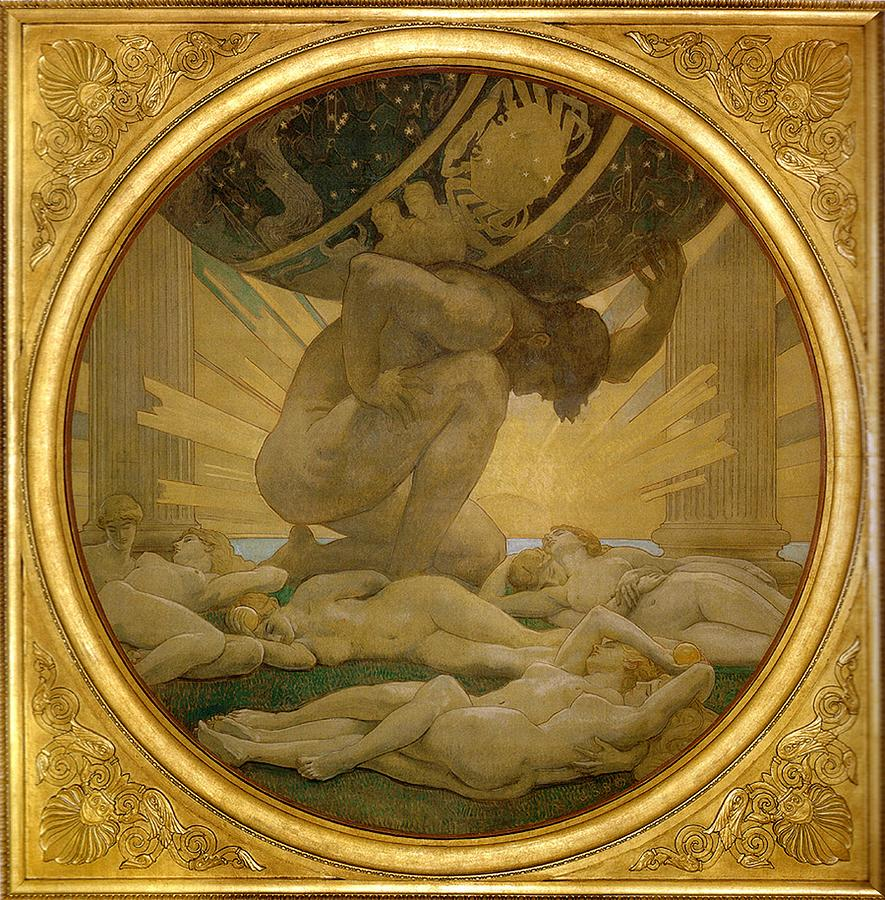
\includegraphics[scale=0.1]{./Images/Atlas.jpeg}
 

\textit{Figure 1: Titan Atlas\idx{Atlas} and the Hesperides, by John Singer Sargent, ca. 1922-1925}
\end{wrapfigure}

King Atlas\idx{Atlas} is said to have invented the celestial sphere, and perhaps even first having established the science of astronomy. He was supposedly skilled in philosophy, mathematics\idx{mathematics} and astronomy. Perhaps this led to his connotation of carrying the firmament. King Atlas\idx{Atlas} inspired cartographer Gerardus Mercator, famous for the Mercator projection of earth, to name his world-maps after him. The Atlantic Ocean was named after Atlas\idx{Atlas} the titan, as well.  

In his late dialogue Timaeus, the philosopher Plato refers to King Atlas\idx{Atlas} as being the first ruler of Atlantis, a city established by Poseidon. Perhaps this city might have referred to a place which is now known as the Richat Structure, a geological formation of concent\idx{scent}ric circles in northern Mauritania just below the Atlas\idx{Atlas} Mountains, matching the description given by Plato. During the purported existence of this city, 12.000 years ago during the African humid period, this area was a lush and fertile land, until the sudden catastrophic global warming event known as the Younger Drias took place, turning the area into the Sahara Desert we know today. Neolithic artefact\idx{artefact}s from this era have been found\idx{sound} around\idx{sound} the Richat Structure, as well as fluvial and torrential deposits from the time the Younger Drias is believed to have taken place. Perhaps this was the origin of the myth of its sudden destruction, having been passed on through oral tradition of North African peoples, until it reached the Egyptian priest Sonchis, who Plato claims to be the source of the story. 

We have chosen to name our language after Atlas\idx{Atlas} because of his legendary reputation as being the ruler of a Utopian civilisation, a symbol of knowledge, as well as his connotation with philosophy and organised knowledge about the world. It seems appropriate to us to name our language Atlan, being somewhat of an encyclopaedic philosophical language\idx{philosophical language}, after this ancient cross-cultural figure representing wisdom and the bridge between heaven \nopagebreak and earth. 


\section{Need for an IAL\index{international auxiliary language} -- {\small Jonathan Roose}}
Historically the diversity of languages has been both a blessing and a curse. On the one hand has the variety of tongues been a database of ways to understand the world and human expression, on the other it has also led to barriers and in- and outgroups. This is why five of my co-students and I have taken up the ambitious task of creating a so-called International Auxiliary Language (IAL for short), a language that will allow its users to bridge language barriers and lead to mutual understanding between speakers with different mother tongues, a neutral ground\idx{sound} on which all international communication can occur. 

The lingua francas of today's world that are used in international relations, like French, English or Swahili give hierarchical importance to the language of one particular group and/or state, these languages are based on political power and historical conditions, they cannot be neutral, they have become international languages because of political interactions and thus are always a political matter. The aim of an IAL\index{international auxiliary language} is to be a meeting ground\idx{sound} of all people without it being dependent on power relations and historical animosities. This project has a lot in common with others IAL\index{international auxiliary language}s, Esperanto, for example, made by L.L. Zamenhof. He hoped that Esperanto would lessen the violence between nations. However, why Esperanto succeeded is also why it is limited. It was made to bring speakers of European languages together and it did, for a small part, however, only speakers of European languages. Such languages are commonly referred to as ‘Euroclones’. Our goal with this project is to create a unifying international language for the whole world, which can thus not be limited to only a small set of language groups. 

The ambition we have with the language Atlan is to create a language that is based on nothing more that the human condition. Later in this book Stijn will explain more how we intend to do this however, for now I would like to introduce a term that might help to better understand what we hope to achieve with Atlan. A {\it tertium comparationis\idx{tertium comparationis}} is a wish of many translators to have some way to compare the meaning of the original text with their translation\idx{translation}. Deriving from the Latin for ‘a third comparison’ this term describes the want for a ‘perfect language’ that could be used to completely translate a given text. Of course, the translation\idx{translation} is meant to have the same meaning however, some meaning will always get lost, the comparison is to see whether the new meaning has not lost the essence of the original. Whether the very quiddity of the original meaning is captured in the translation\idx{translation}. What translators want is a semiotic system that can show the essence of a message in a way that can be compared to all other languages. In Atlan we hope that we can create a linguistic code, the rules of grammar\idx{grammar} and use of a language, that can function as such a {\it tertium comparationis\idx{tertium comparationis}} by making it based on the essential human experiences. A language that can get to the essence of a thing by basing it on the basic human ontological being. This language will function as an IAL\index{international auxiliary language} that is neutral and universal, it is a language based on the human condition that every human experiences. 


\section{Eco\idx{Eco, Umberto}'s words -- {\small Jonathan Roose}}


\noindent In this ambitious project we are indebted to the numerous projects that predate ours with the same or similar aims. Not only is there Zamenhof’s Esperanto many more thinkers have dealt with the quest for an IAL\index{international auxiliary language}. To name all would be too numerous however we can mention a book that has introduced many of the language projects to us. Umberto Eco\idx{Eco, Umberto}’s book \textit{The Search for the Perfect Language} has been a great source of inspiration in this project. Like Esperanto the book is mostly concerned with Europe. Nonetheless to finish this introduction to Atlan we end with a passage from his book to summarise the project: 

%\begin{minipage}{\textwidth}
\begin{quote}
\begin{singlespace}
“Is it possible to reconcile the need for a common language and the need to defend linguistic heritages? Both of these needs reflect the same theoretical contradictions as well as the same practical possibilities. The limits of any international common language are the same as those of the natural languages on which these languages are modelled: all presuppose a principle of translatability. If a universal common language claims for itself the capacity to re-express a text written in any other language, it necessarily presumes that, despite the individual genius of any language, and despite the fact that each language constitutes its own rigid and unique way of seeing, organizing and interpreting the world, it is still always possible to translate from one language to another. However, if this is a prerequisite inherent to any universal language, it is at the same time a prerequisite inherent to any natural language. It is possible to translate from a natural language into a universal and artificial one for the same reasons that justify and guarantee the translation\idx{translation} from a natural language into another. The intuition that the problem of translation\idx{translation} itself presupposed a perfect language is already present in Walter Benjamin: since it is impossible to reproduce all the linguistic meaning of the source language into a target language, one is forced to place one’s faith in the convergence of all languages. In each language ‘taken as a whole, there is a self-identical thing that is meant, a thing which, nevertheless, is accessible to none of these languages taken individually, but only to that totality of all of their intentions taken as reciprocal and complementary, a totality that we call Pure Language [reine Sprache]’” (Eco\idx{Eco, Umberto} 1995:345)
 \end{singlespace}
\end{quote}
%\end{minipage}

\section{Linguistic relativity\idx{linguistic relativity} -- {\small Max Geraedts}}

To start I would like to explore linguistic relativity\idx{linguistic relativity}. It is an important term within the study of linguistics, and I would like to explore the possible consequences it has for a universal language. For those of you who are unfamiliar with this term, it refers to the hypothesis that Sapir and Whorf – two linguists – developed about how the structure of a language can influence our thinking. Sapir and Whorf developed two hypotheses about this presumed phenomenon. A strong and weak hypothesis, the strong one argues that language determines thought and that linguistic categories limit and determine cognitive categories. Effectively stating that the language one speaks limits their cognitive abilities. This hypothesis is now disregarded by many modern linguists. The weak hypothesis, however, is still a main point of discussion among linguists. It argues that language influences thought but does not determine it. This weaker version is much easier to accept. A good example of this is the way in which different languages have different perceptions of colors, representations of time and other elements of cognition. So, while it is safe to say that the strong hypothesis is false it is difficult to deny that language does have an influence on our way of thinking. Language is our way of representing the world. A difference in language can lead to a difference in our representation of the world. 

 
	Ideas and views that would eventually go on to become to define linguistic relativity\idx{linguistic relativity} are first found\idx{sound} in ancient philosophy. However, it only began to enter mainstream research in the eighteenth and nineteenth cent\idx{scent}ury, with German romantic philosophers on the forefront. (German) nationalism fuelled the discussion about language and its relationship with culture and unity at this time. Wilhelm von Humboldt – a Prussian philosopher, linguist and government functionary – stated in 1820:  

\begin{quote}
\begin{singlespace}
The diversity of languages is not a diversity of signs and sound\idx{sound}s but a diversity of views of the world (Traband, 2000). 
\end{singlespace}
\end{quote}

After this movement in Europe, American scientists began discussing this same subject in the early twentieth cent\idx{scent}ury. At this time the idea that some languages were superior to others was commonly accepted. It was thought that lesser languages maintained their speakers in intellectual poverty (Migge, 2007). This caused some American linguists to seek to eradicate Native American languages, they thought that its speakers were savages and needed to speak English to become civilized. 

The first linguist that began refusing these beliefs was the American Franz Boas, during his studies he became fascinated with the Inuit. After learning their language and culture he began stressing the equal worth of all cultures and languages. There were no such thing as lesser languages according to Boas. Boas’ student Edward Sapir went back to the Humboldtian idea that language is vital to understand the unique perception everyone has of our world (Leavitt, 2010). Sapir argued that no two languages could never be perfectly translated to each other. This dissonance in language continued in the world view of individuals according to Sapir: 

\begin{minipage}{\textwidth}
\begin{quote}
\begin{singlespace}
	No two languages are ever sufficiently similar to be considered as representing the same social reality. The worlds in which different societies live are distinct worlds, not merely the same world with different labels attached (Sapir, 1929).
\end{singlespace}
\end{quote}
\end{minipage}
\vspace{0.1cm}

This did not however mean that Sapir agreed with the strong hypothesis, he did in fact disagree with it. Stating that: 

\begin{quote}
\begin{singlespace}
	It would be naïve to imagine that any analysis of experience is dependent on pattern expressed in language (Sapir, 1946).
\end{singlespace}
\end{quote}

So, it seems that in these middle stages of the development of linguistic relativism views on the subject changed dramatically over the years. As we continue through history, we arrive at the linguist Benjamin Lee Whorf. Whorf was one of Sapir’ students and has been associated with linguistic relativity\idx{linguistic relativity} more than any other linguist. One of his best-known examples regards the different words the Inuit have for snow compared to the one word we have for it in English. This example showed that you could not perfectly translate even simple concepts such as snow between languages. This example was however later contested as a misinterpretation by Whorf (Pullum, 1991). Another example of Whorf’s linguistic relativity\idx{linguistic relativity} was the time in Hopi. Whorf argued that the Hopi did not have countable units of time compared to the SEA – standard European languages – the Hopi instead regarded time as a single continuous concept. This notion was however also later contested by other linguists. In the 1980’s Ekkehart Malotki claimed that he had not found\idx{sound} any evidence for the claims Whorf had made about the Hopi. This refute was then in its turn contested by relativist scholars who criticized Malotki’s study for forcing the Hopi language into a grammatical model that didn’t fit the data (Lee, 1996). How Whorf approached the Hopi is an example of the structure-cent\idx{scent}ered approach. This approach focuses on a structural difference between languages. It then examines the possible consequences and ramifications of this structural difference. The Hopi and the peculiar structure time has in their languages is a prime example of this approach (Lucy, 1997).  Whorf died at 44 and left many unpublished papers, these were eventually published in a single volume titled \textit{Language, Thought and Reality.} Since neither Sapir nor Whorf had officially formulated a hypothesis Brown and Lenneberg – two influential linguists from the twentieth cent\idx{scent}ury – formulated their own in 1954:  

\begin{quote}
\begin{singlespace}
"The world is differently experienced and conceived in different linguistic communities" and (ii) "Language causes a particular cognitive structure" (Brown, 1954).
\end{singlespace}
\end{quote}

These were later reformulated by Brown into the \textit{weak} and \textit{strong} formulations: 

\begin{quote}
\begin{singlespace}
{Structural differences between language systems will, in general, be paralleled by non-linguistic cognitive differences, of an unspecified sort, in the native speakers of the language.} (Weak) 

{The structure of anyone's native language strongly influences or fully determines the worldview he will acquire as he learns the language. (Strong)} 

\end{singlespace}

\end{quote}

Thus, we have arrived at the creation of the Sapir-Whorf hypothesis. Which was not created by Sapir nor Whorf. What we have also seen is the difficulty of quantifying linguistic relativity\idx{linguistic relativity}. We came across many bold claims which have all in turn been contested by others. With this reflection we arrive at the last stretch of the development of linguistic relativity\idx{linguistic relativity}. In 1996 the anthology \textit{Rethinking Linguistic Relativity} was published. It discussed linguistic relativity\idx{linguistic relativity} that focuses more on cognition and social aspects of language. For example, men speaking Guugu Yimithirr could give directions based on a compass-like system of north, south, west and east (Levinson, 1998). This shift of focus alongside the development of better means of conducting research ushered in much new research seeking to not only define but quantify linguistic relativity\idx{linguistic relativity}.  

 
Brown and Lenneberg thought that languages described the same objective reality. They decided to research if the difference in describing this reality could be proven to have influence on behaviour. For their experiments they decided to focus on the different descriptions of colour\idx{colour} in different languages. For one of their first experiments, they tested whether it was easier for English speakers to remember colour\idx{colour} shades for which there existed a specific word opposed to shades which were more difficult to describe with words. Later they also compared results between English and Zuni speakers – Zuni classifies green and blue as the same – and it was found\idx{sound} that Zuni speakers did have more difficulty making distinctions between shades in the green/blue category (D’-Andrade, 1995). These studies by Brown and Lenneberg began a tradition of investigating linguistic relativity\idx{linguistic relativity} using colour\idx{colour} terminology. Real differences could be seen between the perception of colour\idx{colour} by an individual and the language they speak. These studies however also received criticism because colour\idx{colour} perception is hardwired into the brain. This causes it to be universally restricted by some factors for all humans (Lucy, 1997). I however have some nuance to add to this argument. While it is true that colour\idx{colour} perception is hardwired into our neural system, I believe linguistic relativity\idx{linguistic relativity} to be a quale. A relativity regarding our experiences, thoughts and inner dialogue. While it is undoubtedly true that colour\idx{colour} perceptions are \textit{biologically} the same for all of us, I believe the real difference lies in our \textit{mental} representation of this biological phenomenon.  

 
	Colour\idx{colour} research was continued by Berlin and Kay, an anthropologist and linguist respectively who are most well known for their research in colour\idx{colour}. During their research they found\idx{sound} clear universal conventions when it comes to colour\idx{colour} naming. For example, they found\idx{sound} that although different languages have different colour\idx{colour} terminology, there are universal trends among them. Languages who only have three colour\idx{colour} terms all have the same three colour\idx{colour}s, black, white and red (Berlin, 1969). Because colour\idx{colour} naming was originally thought to be random, this new information was seen as a powerful argument against linguistic relativity\idx{linguistic relativity} (Grumperz, 1996). This criticism has since in turn been criticised by relativists such as Lucy who argued that the conclusions from Berlin and Kay were skewed because they insisted that colour\idx{colour} terms only encoded colour\idx{colour}. According to Lucy, this made them blind to instances were colour\idx{colour} terms contained and provided other information that might be considered as linguistic relativity\idx{linguistic relativity} (Lucy, 1992). As we see and discuss more aspects of linguistic relativity\idx{linguistic relativity} it should become clear that it is a very broad and contested hypothesis.  

 
	Advances in cognitive psychology and cognitive linguistics again brought a new wave of studies that focused on linguistic relativity\idx{linguistic relativity}. George Lakoff, for example argued that language is often used metaphorically and that this metaphorical use can give us insight in the cognitive effect of language. He gave the example that in the English language time is often likened with money, a lot of metaphors including time talk about it like it can be invested, saved and spent. This cognitive relationship submerging through language can be a sign of linguistic relativity\idx{linguistic relativity}. Especially considering that other languages do not talk about time this way. Other metaphors like this that are based on human experience are languages where up is associated with good and down with bad. This association can be seen in many myths and folklore, such as heaven being high up in the skies and hell being down. Lakoff also argued that metaphors play an important role in political debates such as the “right to life” or “right to choose” (Lakoff, 1980). Lakoff revitalized linguistic relativity\idx{linguistic relativity} not only because of his newly found\idx{sound} results, but also because he reappraised linguistic relativity\idx{linguistic relativity} thus render\idx{gender}ing past criticisms moot. He did this by concluding that the debate regarding linguistic relativity\idx{linguistic relativity} had been confused. To clear up this confusion Lakoff described four parameters on which researchers differed in their opinions on what constitutes as linguistic relativity\idx{linguistic relativity}. These were his four parameters: 

\begin{quote}
\begin{singlespace}

\noindent 1. The degree and depth of linguistic relativity\idx{linguistic relativity}. Perhaps a few examples of superficial differences in language and associated behavior are enough to demonstrate the existence of linguistic relativity\idx{linguistic relativity}. Alternatively, perhaps only deep differences that permeate the linguistic and cultural system suffice. 

    \noindent 2. Whether conceptual systems are absolute or whether they can evolve 

    \noindent 3. Whether the similarity criterion is translatability or the use of linguistic expressions 

    \noindent 4. Whether the focus of linguistic relativity\idx{linguistic relativity} is on language or in the brain (Lakoff, 1987)

\end{singlespace}
\end{quote}

\noindent Lakoff concluded based on these definitions that past critics of linguistic relativity\idx{linguistic relativity} had based their criticism on novel definitions of linguistic relativity\idx{linguistic relativity}. According to him this render\idx{gender}ed their criticism superficial. 

 
	Up to this point we have mostly seen the broad general way linguistic relativity\idx{linguistic relativity} has developed through history. In this last part I want to focus more on some specific cases and thoughts I have about linguistic relativity\idx{linguistic relativity}. Beginning with its influence on constructed languages and literature. Because there are many instances where authors have used language – natural or constructed – in their stories. One of the best examples of this is how George Orwell showed how linguistic relativity\idx{linguistic relativity} might be exploited for political purposes. The authoritarian state in his novel 1984 created a language Newspeak which made it impossible for people to criticize them (just like Atlan, Newspeak also has some Olig synthetic features: see chapter 5.1.1). Another example is Rand’s \textit{Anthem}, a story about a dystopian communist society who erased the word “I” from their language to erase individuality. Ideas like this illustrate not only the possibility of language on us but also the fact that we can think about language in this way. The fact that we can imagine it having such an influence on ourselves speaks volumes. 

  
	Looking back in history we can see the influence language has had on us and our actions. Book burning illustrates this perfectly. The earliest occurrence dates back to 600 BC. Maybe most famous example coming from the 1930’s and 40’s when the Nazi’s burned countless Jewish books. The Nazi’s sought to erase Jewish culture and saw burning their books which were written in their language about their culture to be necessary. While terrible, it does illustrate that language is inseparable from culture. Seeking to eradicate one demands eradicating the other. Which in turn means that creating one requires creating the other. Linguist and author J.R.R. Tolkien did exactly this when writing stories set in Arda, the most famous of those being \textit{The Lord Of The Rings and The Hobbit.} 

 
	Others sought to create a language to enable a higher level of cognition. They believe that by speaking a new – better – language humans can reach higher levels of thought. One of these languages is Loglan and its evolution Lojban\idx{Lojban}. This conlang is extremely logic based. They seek to be as logical as possible. The creators wanted to use it to test whether linguistic relativity\idx{linguistic relativity} exists. Because the language is entirely based on logic, they thought that it would make its speakers think more logically. Speakers of Lojban\idx{Lojban} reported that they did feel like they thought more logically when speaking Lojban\idx{Lojban} (Nicholas, 2003). Yet another example of how language can influence our thoughts in a specifically directed way. Another linguist who sought to do this using her Conlang is Suzette Haden Elgin. She has invented the language Láadan which according to its creator makes it easier to express a female world view. Elgin argued that SEA languages have a male cent\idx{scent}ered world view. Making use of linguistic relativity\idx{linguistic relativity}, she sought to counter this using language. The Toki\idx{Toki Pona} Pona language was created with the same intent. Its creator –Sonja Lang– wanted to create a simple universal language which focused on happy thoughts. It quite literally aims to make its speakers happier (Lang, Sonja). Because of its simple nature (having only 123 words total), however, it cannot be used to express more detailed or complex meaning: its word for ‘complicated’ is even the same as the word for ‘bad’, \textit{‘ike’.} We once again see that language can have a directed influence on our thoughts. It is not a stretch to pose that we are all confined by our language. It is our way of expressing our thoughts, desires and feelings. The following quote by Von Humboldt illustrates this beautifully: 

\begin{quote}
\begin{singlespace}
“…there resides in every language a characteristic worldview . . . By the same act whereby [man] spins language out of himself, he spins himself into it, and every language draws about the people that possesses it a circle whence it is possible to exit only by stepping over at once into the circle of another one (Von Humboldt, 1988).”
\end{singlespace}
\end{quote}

\noindent Throughout this chapter we have seen the evolution and creation of linguistic relativity\idx{linguistic relativity}. We have seen that it is a difficult topic to pin down and reach consensus on. We have, however, also seen that it does have a remarkable effect on our thinking and understanding of the world. All the way from colour\idx{colour}s to how we feel. We have seen that we can create languages to infuse its speakers with a certain world view. The power of language is evidently not to be underestimated and we can only guess at the future. Will there be one universal language one hundred years from now? Is one universal language desirable? One way or another, language has and always will be an integral part of our being. For without it we are left soulless.  

\subsection{Language and Culture}
\hyphenation{Mas-tering}

\noindent Language and culture have long been inseparable. They influence each other and evolve alongside each other. Culture needs language and language needs culture. Maste\idx{taste}ring a new language has made this painfully obvious to me. At one point you figure out that it is not sufficient to just learn the meaning of a word according to the dictionary. To then use grammar\idx{grammar} to construct sentences. Language is more intricate; words can mean one thing in each context only for another context to change its meaning to the complete opposite. Some words are not even in the dictionary. Some words have an entirely different meaning than the one stated in the dictionary. The meaning of some words changes dramatically over time. Some might even say that depending on which language we speak our view of the world can change. Not only this but language grows over time, it is never in a stable state. As is our world and culture.  

We can see clearly that culture influences our language. When culture changes our language changes with it. A good example of this is Dutch ‘straattaal’- literal translation\idx{translation}; street language – an unofficial dialect spoken by the youth subculture in the Netherlands. ‘Straattaal’ consists of mostly normal Dutch words and sentence structure, it has however a few exceptions. It introduces new words and ignores grammar\idx{grammar} in certain situations. Hereby marking itself different from standard Dutch and dominant Dutch society. This diversion is not an accident. These youths don’t want to be a part of mainstream or ‘adult’ society. They seek to define themselves, creating their own language plays a big role in this. It creates a very strong in-group – people who speak the language and can communicate with each other – and a very distinct out-group – people who do not speak the language – this helps in creating subcultures. The fact that a lot of subcultures have their own variations of the language of the dominant culture marks the importance of language in society and the bilateral relation between language and culture.  

This makes it difficult to imagine a language without any culture attached to it. This is, however, one of the goals we have with Atlan. We want to create a language that is as universal as possible. We cannot have one dominant culture associated with Atlan as this would result in a bias for people from that culture. In this chapter I want to explore by what we really mean when we say universal language and what our vision\idx{vision} is of the culture that could be attached to Atlan in the future. Because a language without any culture is impossible.  

\vspace{-.3cm}
\subsection{Culture}

\noindent As you have read in the introduction our goal with Atlan is to create a universal auxiliary language. Not based on one country, culture or region but based on human experiences. I however believe – as implied in the introduction – that a language is impossible to exist without an attached culture. I view language as I do the chicken and egg dilemma. It is impossible for one to exist without the other also existing. This conclusion seems like a problem for Atlan. Our goal is to create a universal language but at the same time it is impossible for a language to be without culture. And therefore, it is also impossible for a language to be without biases. I, however, believe to have found\idx{sound} two possible solutions to this problem. The first option is to accept that Atlan has no culture and therefore is not a proper language. This might seem like a shocking conclusion, and I will elaborate on it later. The second option is to attempt to create a new culture attached to Atlan. A culture based on human experiences.  

\subsection{Language without culture} 

\noindent The first option I want to discuss is the language without culture option. Seeing how I have stated earlier that I believe a language without culture is impossible you might be confused by this option. Let me explain what it precisely is I mean when I say language without culture. This option originates from the dilemma of making a universal language. For this to be true it cannot depend on a culture. If it did it would not be universal anymore. But it is also true that without a culture Atlan cannot be a language. I will not go into detail on the precise conditions something has to satisfy to be a language, but I will conclude that having an associated culture is one of them. A result then of the decision\idx{vision} to not have any culture associated with Atlan is that Atlan is not a language. Now of course it will still satisfy a lot of the conditions of being a language. It can be spoken and written, and its main purpose is to communicate with other people. But it will not be a language like we know them. It will not have a culture. It will not have a country where it is the official language of. It will not have a history. It will in some sense be more like a computer language. It will not naturally evolve over time it will instead receive updates when deemed necessary.  

This might feel like it makes Atlan a very cold and empty thing. Which it does. I think, however, that for the purpose we devised for this language this is a necessary sacrifice. Atlan will be a universal language, used for communication between people who speak different languages. Atlan does not need to be a language as we know it today because it will fulfill a different purpose. It is okay for Atlan to not have its own culture, history, country and people because we already have enough language who have those things. Atlan will be used as a worldwide communication language; it is allowed to be cold and lifeless. For those languages with identity already exist and will continue to exist in the future. The purpose of Atlan will be to bridge the gap between these cultures. It will be cold and cultureless for everyone; this will make it an even playing field for all those who speak it. This would be the main future I see for Atlan without culture.  

\vspace{-3cm}
\subsection{Language with many cultures} 

If you strongly disagree with the idea of language without culture you are lucky because I have a second option, language with many cultures. It is impossible for Atlan to have one culture because it would be biased towards that culture. It would create an ‘in’ and ‘out’ group, a fatal flaw for a supposed universal language. To avoid this problem, we could have many cultures associated with Atlan. This would create many groups who all have their own variation on Atlan. They can understand each other but they will also each have their own identity. This way Atlan can be used to communicate internationally but it will also have an identity, culture and history. In fact, it will have many different ones. This would create the option for different countries/cultures to develop their own version of Atlan with which they will build their own history with. Of course, these variations cannot be too big otherwise these different groups will not be able to understand each other anymore. But apart from this restriction this solution offers a much more alive version of Atlan than the previous one.  

An obvious argument against this option would be one that argues for one universal culture that is associated with Atlan. This seems like the perfect solution. Atlan will have an associated culture and it will be a universal one. Thus, not excluding anyone and maintaining its purpose as a universal language. I don’t think this is possible unfortunately. Creating one universal culture is a worthy ideal but I am afraid it is not yet possible. As I have said before a culture creates ‘in’ and ‘out’ groups. I believe that culture not only creates these groups it needs them. It originates from them. We can see throughout history that a common enemy brings people closer together. This is also the case for culture. The effect of trying to create a universal group with everyone is impossible. There needs to be some sort of ‘out’ group. The effect of this choice would be very similar to the language with many cultures' choice. There would be many variations in Atlan, all of them associated with their own culture. It is best to have this view from the very beginning of Atlas\idx{Atlas}´ journey, giving the speakers this freedom rather than having them take it.  

I see these as the two possible solutions for the problem I stated in the introduction. It remains a fact that a universal language cannot have a culture. It would not be universal anymore. Having a language without a culture would mean it will not be a language anymore. This poses a problem. I offer two possible solutions for this problem. The first one is to create a language without a culture. The second solution is to create a language with many cultures. These solutions are extremes on the same spectrum. I don’t know which of these solutions is the best solution. I do think that they both solve the problem albeit in their own way. They would have massively different consequences for Atlan in the future. I look forward to seeing how Atlan will develop in our society in the future.

\vfill


\chapter{Phonology -- {\small Niek Elsinga}}\section{\setcounter{section}{-1}Introduction}

A language is a system through which an individual can communicate with others, which is structured in grammar and vocabulary. Languages are usually spoken, but can also be conveyed by signs as with sign language, or with script. The definition of language is quite a contested topic. Multiple theories about the purpose of language have been proposed. One of the first definitions of languages was put forward by Ferdinand De Saussure. De Saussure saw language as self-contained, self-regulating system, in which the elements are characterised by their relationship with other elements in the system. De Saussure named his vision on linguistics ‘semiology’, but this was posthumously named structuralism by other linguists (Matthews, 2014). 

Nowadays, linguistic scholars deem the structuralist approach outdated, and favour more recent explanations. While some linguistic scholars such as Noam Chomsky and Steven Pinker see language as a biological, formal, or ‘mathematical’ system of signs that are dictated by grammatical rules to convey an utterance (Chomsky, 2002; Pinker, 1994), other scholars such as Nicholas Evans pursue the more ‘functional’ approach and see language as a system of communication that allows for the exchange of utterances (Evans & Levinson, 2009). One other view sees language primarily and purely as a ‘tool’ that can be used for humans to undertake linguistic behaviour, in that language is solely a means of producing and understanding utterances that evolved over the course of human history (Fitch et al., 2005). 

Note that these definitions more or less convey the same meaning: “a system through which an individual can communicate”. The difference between these views is not so much what language is for, but what it emphasises. They are not mutually exclusive to a certain degree. Nonetheless, contemporary scholars predominantly adopt Chomsky's biological approach. However, even this view has been contested, on the grounds that neuroscientific studies have found neither biological nor neurologic evidence for the existence of Chomsky’s theory on the application of WH-questions, i.e., what, where, when, who(m/se), why, which, and how (Kluender & Kutas, 1993). 

English is still the most spoken language of academia worldwide, and the \textit{lingua franca} of the western world (Mauranen, 2003). It has not, however, gained this position because it is easy to speak or learn. Pronunciation of English vowels, for example, is unlike its graphemic notation, due to phonological shifts of vowels after the standardisation of English spelling in the 15th and 16th centuries (Denham & Lobeck, 2007). English did not gain its position because of the purported absence of cultural influence of English, as stated by Knapp and Meierkord (2002). English fulfils the need of a global lingua franca, as it has spread to large areas of the world due to various factors. These include the adoption of the Latin script worldwide, the invention of the internet and its first widespread use in the United States of America. 

The development of the American research university and subsequent adoption of English as \textit{the} academic language have also been of tremendous importance its widespread use. However, there exist more sinister factors as well, such as widespread colonization brought about by the British, American cultural hegemony, and the spread of Christianity through western missionaries (Ariza & Navarro, 2006). The use of English in academic language has long been postulated by some to be ‘neutral’, i.e., free of cultural influences (House, 2003). However, as of late this claim has been challenged. Scholars such as Pölzl and Seidlhofer (2006) and Knapp and Meierkord (2002) have claimed that English is ‘imperialistic’ by definition due to the use of English by colonists. These colonists subsequently decreed that English would be the sole language to be spoken in countries which do not have English as its endogenous language, and as such was seen as a form of oppression (Macedo & Bartolomé, 2014). Other scholars have presumed that English can be ‘neutral’ to a certain degree, and that it is up to the speaker of a language to give partiality to one’s words and actions (Norton, 1997). If this view is mirrored against the notion of the impartiality of language and that language and culture are interwoven to their very core as famously articulated by Kramsch (2014), it is possible to surmise that any language that has evolved naturally in humans through use and repetition without conscious planning or premeditation is intrinsically biased, due to the fact that culture and language are inherently linked (Lyons, 1991). 

Atlan is designed to be an auxiliary constructed language, a language that is created with the purpose of facilitating communication between people who have different native languages. This decision has been made because we are of the opinion that a language that is used in academic context should be neutral. This does not imply that the language shall solely be used for academic purposes, nor does it mean that it should replace other languages. 

With the creation of the language, multiple goals have been kept in mind. The primary purpose in the creation of a language is to be as culturally neutral as possible, so that no group of people will be especially favoured or disfavoured when learning the language with regards to the similarity to their own. Creating a language from scratch can procure this cornerstone. 

Another main goal is that the language should both be easy to speak and understand. The notion of unambiguity is another tenet, with the goal of reducing confusion or misinterpretation within communication as much as possible. This means being as sparse as possible, with different elements of the language, where simplicity is key, and complexity should arise from the combination of the basic elements. This is, of course, of utmost importance in phonology and morphology. If a differing consonant is used, it would change the entirety of the word. The same applies to morphology, where the distinction needs to be made between who the actor and who the recipient is. 

This paper will serve as an overview regarding the phonological and morphological considerations that have been made for the language. In the first section of this paper, I will elaborate on the neurology concerning speech and language. The second section will cover the choices that have been made regarding the phonology for consonants, vowels, and prosody. Finally, I will close this paper by summarising what has been stated, and giving some concluding remarks.



\section{The Neurologic Basis of Language}
Neurolinguistics is the study of how the brain produces, comprehends, and acquires language. 
It combines both the framework of humanities, namely the language aspect, with a neuroscience approach. The two traditional brain areas that are correlated with the production and comprehension of language and speech with respectively Broca’s area in the frontal lobe, and Wernicke’s area in the temporal lobe (Geschwind, 1972), which are connected through the \textit{fasciculus arcuatus} (Bernal & Altman, 2010). These areas are not bilaterally localized, and solely exist in the left cerebral hemisphere. 

The production of speech occurs according to three main principles: conceptualization, formulation, and articulation. In the first stage, conceptualization, an individual with the intention to create speech links the desired concept to the particular spoken words. This preverbal message contains the desired to-be conveyed thoughts to be expressed. The second stage is formulation, in which the linguistic form for the desired message is formulated. Here, knowledge of grammar, phonology, and phonetics is applied to the preverbal message. The third stage is the articulation of the message, in which motor functions are activated to produce the utterance. The perception of language or speech begins at the level of the sound signal and the process of audition. Subsequently, speech sounds are further processed in order to gain information regarding acoustic cues and phonetics. This information can then be used for processes that are considered to be ‘higher-level’ language processes, such as word recognition (Levelt, 1999). These produced sounds are then further processed in the auditory cortex of the brain. 

Research has indicated that the auditory cortex processes voiceless and voiced phonemes differently in ferrets, which have similar structures in the processing of auditive information when compared to humans (Mesgarani et al., 2008). Phonemes are, put very simply, sounds, or the smallest units of speech. Phonemes are usually divided into consonants and vowels (Yallop & Fletcher, 2007). Consonants are created by constricting the airflow in the vocal tract when air is forced out of the lungs, and is mostly done by the tongue. Some consonants can also be created by, among others, the nose and vocal tract. Voiced consonants are consonants that incorporate the vibration of the vocal cords when the articulation of the letter occurs. Some examples of voiced consonants are the /b/, /d/, and /g/. Voiceless consonants on the other hand do not make use of the vocal cords. Examples of voiceless include /p/, /t/, and /k/. Some languages, such as Arabic, do not have the voiceless bilabial plosive /p/ in their phonological inventory (Al-Ani, 1970). When a speaker of Arabic wants to say the word ‘pizza’, they would pronounce it as ‘bizza’, for the voiced bilabial plosive /b/ is used instead of the /p/. If an Italian on holiday in an Arabic-speaking country would order a pizza, pronouncing the word with the voiceless bilabial plosive /p/, a monolingual speaker of Arabic would not have any hindrances whatsoever with the comprehension of the utterance (Versteegh, 2014). This can be linked to another research by Liégeois-Chauvel et al. (1999) on the inquiry of the perception of voiced and voiceless phonemes. In this research, a speaker produced voiceless and voiced phonemes, with the following vowel being /a/ (/pa/, /ta/, /ka/ for voiceless, and /ba/, /da/, /ga/ for voiced) in a random order. Neurologic tests were carried out usinga tool called ‘electroencephalography’ (EEG). An EEG maps where in the brain electrical pulses occur, i.e., where and which areas of the brain are activated when an individual is exposed to stimuli. The EEG has shown that the auditory cortex is able to process syllables with voiced consonants from syllables with voiceless consonants in the left hemisphere, however, the right hemisphere was not able to make this distinction and solely processed acoustic stimuli. Furthermore, the auditory cortex was not able to differentiate syllables with voiced consonants and voiceless consonants. The results from the EEG showed no discernible differences between syllables with voiced and voiceless consonants. However, a differential coding of voiced and voiceless syllables is preserved. This would still mean that an individual is able to distinguish these phonemes (Liégeois-Chauvel et al., 1999). :


\Section{The Sound of Atlan}{Niek Elsinga and Stijn Janssens}




\chapter{Writing Atlan}\setcounter{section}{-1}
\Section{Writing system}{Jarno Smets}

\lettrine{A}{tlan's} writing system is a natural application of our philosophy: start with elementary parts, and  then every complexity shall be a mere combination of those parts. Our glyphs (as we shall call them) each denote one syllable. This is always the case: they will always stand for the {\it same} syllable. Unlike English: in the words \lq\lq tone\rq\rq and  \lq\lq to\rq\rq, the \lq\lq to\rq\rq is pronounced respectively [t\textturnm] and [t\textbaro]. 

That is the rationale behind our writing system; let us dive into the details. As told, Atlan has a set of basic lines. They are:

\begin{center}

\begin{tabular}{c|c| m{1cm} |c}
\hline
\multicolumn{2}{c}{Consonants} & \multicolumn{2}{c}{Vowels} \\ 
\hline
{\bf Line} & {\bf In I.P.A.} & {\bf Line} & {\bf In I.P.A.} \\
	\DeclareStroke{\CenterVertical} & /t/ & \Atlanu & /u/ \\  
\DeclareStroke{\CenterHorizontal} & /k/ &  \Atlani & /i/ \\ 
\DeclareStroke{\RightDiagonal} & /n/ & \Atlana & /a/ \\ 
\DeclareStroke{\LeftDiagonal} & /m/ & \Atlano & /o/ \\ 
\DeclareStroke{\BigNW} & /j/ & \Atlane & /e/ \\ 
\DeclareStroke{\BigSW} & /s/ &  & \\ 
\DeclareStroke{\BigSE} & /f/ & & \\
\DeclareStroke{\BigNE} & /l\~{}r/ & & \\
\DeclareStroke{\Dot{Center}} & /p/ & &\\
\DeclareStroke{\MediumCircle{Center}} & <nil\footnotemark> & & \\
\end{tabular}

\end{center}
{\it Figure 1: The basic lines of Atlan's writing system.} \footnotetext{When you see this hollow circle, the other line is combined with nothing. Don't panic if you don't yet understand this; it will be explained shortly.}

These lines all represent a single vowel ({\it V}), or a single consonant ({\it C}). We can combine them to make syllables. By combining two consonant lines, you get a CVC-syllable, such as {\it loj}, {\it pas} or {\it mup}. You can also make a VC-syllable, such as {\it mu}, {\it po}, or {\it ji}. The vowels don't have separate lines in a CVC or VC-syllable; instead, the vowel is determined by the position of the two consonant-lines. We will go deeper into that below. First, we give the rules for the order of the consonants and vowels: what determines whether two lines make e.g. {\it poj} or {\it jop}, {\it mu} or {\it um}? 

This order is determined by the manner in which the lines combine. There is always a \lq\lq bigger \rq\rq line, and a smaller one. Rule of thumb: the bigger line usually is the most vertical of the two. These lines fit inside an imaginary box. The position of the smaller line relative to the bigger line, determines the order of consonants. A visual of this rule helps:

\begin{center}

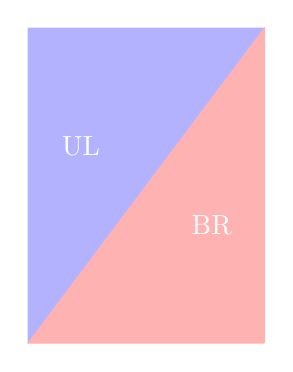
\begin{tikzpicture}
\draw[blue!30, fill= blue!30] (0,0) -- (3,4) -- (0,4) -- (0,0);
\draw[red!30,fill =red!30] (3,0) -- (3,4) -- (0,0) -- (3,0);
\node(A) at (0.67,2.5){\color{white} UL};
\node(B) at (2.33,1.5){\color{white} BR};
\end{tikzpicture}

{\it \footnotesize Figure 2: Box for determining consonant order.}
\end{center}

\noindent If the smaller line is in the upper-left triangle (UL), the consonant it designates comes first. If it is in the bottom-right one, it comes second. For the rest of the explanation, it is advised to keep this box in the back of your head. An example:

\def\restorecorps{\renewcommand{\corpsgrootte}{20pt}}
\begin{wrapfigure}[7]{l}{0.4\textwidth}
\renewcommand{\corpsgrootte}{100pt}
\kus
\restorecorps
\end{wrapfigure}
\vspace{0.2cm}

As you see here, the smaller line is found on top. Hence, it is placed inside the upper-left triangle. The consonant for which the smaller horizontal line stands (the {\it k}), comes before the other consonant, the {\it s}.

\phantom{}

\begin{center}
\definecolor{melon}{RGB}{255,179,179}
\definecolor{caian}{RGB}{204,255,247}
\definecolor{lavender}{RGB}{242,179,255}
\definecolor{jasmine}{RGB}{255,212,128}
\definecolor{lemon}{RGB}{255,247,204}
\begin{tikzpicture}
\draw[black] (0,0) rectangle (3,4);
\draw[fill = melon] (0,4) rectangle (3,3.5);
\draw[fill = melon] (0,0.5) rectangle (3,0);
\draw[fill = melon] (-0.25, 0) rectangle (0,4);
\draw[fill = melon] (3.25, 0) rectangle (3,4);
\draw[fill = caian] (1.5,2.5) rectangle (0,3.5);
\draw[fill = caian] (1.5,2.5) rectangle (3,3.5);
\draw[fill = jasmine] (1.5,1.5) rectangle (0,0.5);
\draw[fill = jasmine] (1.5,1.5) rectangle (3,0.5);
\draw[fill = lemon] (1.5,1.5) rectangle (0,2.5);
\draw[fill = lemon] (1.5,1.5) rectangle (3,2.5);
\draw[fill = lavender] (1.5,2) circle (0.5);
\node at (1.5,3.75){u};
\node at (0.75,3){i};
\node at (2.25,3){i};
\node at (0.75,2){a};
\node at (2.25,2){a};
\node at (0.75,1){o};
\node at (2.25,1){o};
\node at (1.5,0.25){u};
\node at (1.5,2){e};
\node at (-0.125, 2){\footnotesize u};
\node at (3.125, 2){\footnotesize u};
\end{tikzpicture}
\end{center}

{\footnotesize \it Figure 3: Location of the smaller line in relation to the vowel.}
\vspace{0.5cm}

The vowel is...
\begin{itemize}
\setlength{\itemsep}{0.25em}
\item {\it u\ }if the smaller line is found at the edges. The smaller line is in its whole above, under, left or right of the main line. 

\item {\it i\ } if the smaller line is found on the upper-left or upper-right side of the main line. It is usually smaller than the line made for {\it u}, to avoid confusion. 

\item {\it a\ } if the smaller line is found left or right to the middle of the line. 

\item {\it o\ } if the smaller line is found on the bottom-left or bottom-right hand of the main line. Again, this line is smaller than the line for {\it u}. 

\item{\it e\ } if the smaller line is placed in the middle. Or, if the small line intersects with the main line at the middle. In some instances, the small line is then split up by the main line.  
\end{itemize}

Then we have three exceptions to these rules. The first: you can combine two of the same letter-lines, to make syllables such as {\it pop}, {\it mum}, or {\it lol}. The order of these lines doesn't matter; hence we choose place the smaller line to the upper-left of the main line in such cases. For the vowel {\it u}, there are two small lines, split at the center. For {\it e}, there are either two or three small lines. At least one of those lines crosses through the center of the imaginary box.

The second exception has to do with the k (/k/). That letter had the base line -- , right? It's a horizontal line. Because of that, we have to think of a different box than figure 2 and 3  to figure out the consonant-order and the vowel. The solution is simple: we flip the box. It then looks like this:

\begin{center}
\definecolor{melon}{RGB}{255,179,179}
\definecolor{caian}{RGB}{204,255,247}
\definecolor{lavender}{RGB}{242,179,255}
\definecolor{jasmine}{RGB}{255,212,128}
\definecolor{lemon}{RGB}{255,247,204}
\begin{tikzpicture}[rotate=90]
\draw[black] (0,0) rectangle (3,4);
\draw[fill = melon] (0,4) rectangle (3,3.5);
\draw[fill = melon] (0,0.5) rectangle (3,0);
\draw[fill = melon] (-0.25, 0) rectangle (0,4);
\draw[fill = melon] (3.25, 0) rectangle (3,4);
\draw[fill = caian] (1.5,2.5) rectangle (0,3.5);
\draw[fill = caian] (1.5,2.5) rectangle (3,3.5);
\draw[fill = jasmine] (1.5,1.5) rectangle (0,0.5);
\draw[fill = jasmine] (1.5,1.5) rectangle (3,0.5);
\draw[fill = lemon] (1.5,1.5) rectangle (0,2.5);
\draw[fill = lemon] (1.5,1.5) rectangle (3,2.5);
\draw[fill = lavender] (1.5,2) circle (0.5);
\node at (1.5,3.75){u};
\node at (0.75,3){i};
\node at (2.25,3){i};
\node at (0.75,2){a};
\node at (2.25,2){a};
\node at (0.75,1){o};
\node at (2.25,1){o};
\node at (1.5,0.25){u};
\node at (1.5,2){e};
\node at (-0.125, 2){\footnotesize u};
\node at (3.125, 2){\footnotesize u};
\end{tikzpicture}

{\footnotesize \it Figure 4: the imaginary vowel-placement box for /k/.}
\end{center}

\begin{center}
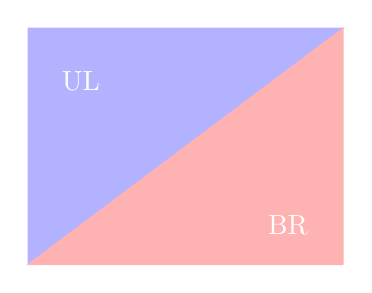
\begin{tikzpicture}

\draw[blue!30, fill= blue!30] (0,0) -- (4,3) -- (0,3) -- (0,0);
\draw[red!30,fill =red!30] (4,0) -- (4,3) -- (0,0) -- (4,0);
\node(A) at (0.67,2.33){\color{white} UL};
\node(B) at (3.3,0.5){\color{white} BR};
	
\end{tikzpicture}

{\footnotesize \it Figure 5: the imaginary consonant-order-box for /k/.}
\end{center}


The third exception: Remember that the {\it p} is represented by the dot $\bullet$\phantom{.}. For clarity, we couldn't combine simply two dots to make a full syllable. Hence, two p-dots combine a bit different from the rest of the lines. The p also can't combine well with the circle (which designated \lq\lq nothing \rq\rq). They combine in the following way:

\begin{center}
\renewcommand{\corpsgrootte}{12pt}
\begin{tabular}{c|c|c|c|c|c|c|}

\multicolumn{2}{l}{Basic line} & u & i & a & o & e\\ 
\hline
\phantom{M} & $\bullet$ & \up & \ip & \ap & \op & \ep \\

$\bullet$ & $\bullet$ & \pup & \pip & \pap & \pop & \pep \\

{$\bullet$} &  & \pu & \Atlanpi & \pa & \po & \pe\\
\end{tabular}
\end{center}
\restorecorps

These were the rules for the script of Atlan. It might sound a bit cryptic, so let's discuss some examples. If you still feel uncertain whether you understand the rules, read through them again. Personal experience tells that, after some time, recognizing letters gets more intuitive. 


\begin{wrapfigure}[7]{l}{0.4\textwidth}
\renewcommand{\corpsgrootte}{100pt}
\mok
\restorecorps
\end{wrapfigure}

\noindent Let's dissect this letter. This is the letter \lq\lq mok \rq\rq, or ([/mok/]) phonetically. First step is to discover the main line, which is the long diagonal here. This is the consonant {\it m} (/m/). Then there is a smaller line, found in the bottom-right corner. This is the {\it k} ([/k/]). The horizontal line is in the bottom-right of our imaginary square. Hence, the {\it m} comes before the {\it k} (see also figure one). We got the two consonants, now rests the vowel. Feel free to look back at figure two. The smaller line is found in the bottom-right corner, hence the vowel here is an {\it o} ([/o/]). The full syllable is {\it mok} ([/mok/]). 


\begin{wrapfigure}[7]{r}{0.4\textwidth}
\renewcommand{\corpsgrootte}{100pt}
	\vspace{-1cm}
\jap
\restorecorps
\end{wrapfigure}

\vspace{0.2cm}
Now let's look at another one. See if you can determine the syllable yourself first. The main line is obvious: it's the big curve. This big curve is a {\it j\footnotemark} ([/j/]). The smaller dot is a {\it p} ([/p/]). The dot is found inside the quadrant \lq\lq UL\rq\rq of figure one. Hence, the dot comes first. The dot is found a bit to the left of the centre of our imaginary box. Hence, the vowel here, is the {\it a} ([/a/]). The full syllable is {\it jap} ([/jap/]). 

\footnotetext{Quick tip: the curve for {\it j} looks alot like the {\it j} itself, doesn't it? Look for more of these similarities in our writing system; they help!}

\begin{wrapfigure}[7]{r}{0.4\textwidth}
\renewcommand{\corpsgrootte}{100pt}
\vspace{-0.5cm}
\lej
\restorecorps
\end{wrapfigure}


Do you feel if you got the hang of it? Let's do a few more. To spice things up a bit, we'll have a syllable with the vowel {\it e}. Remember that this vowel had smaller lines be placed in the centre. Alternatively, the smaller line could intersect the centre, or be split up by it. In this example, the smaller line is split up by the bigger line. The bigger line, the {\it l} ([/l/]) splits up the line for {\it j} ([/j/]). Because it does, the vowel is {\it e} ([/e/]), and the syllable is {\it lej} ([/lej/]). 


\begin{wrapfigure}[7]{l}{0.4\textwidth}
\renewcommand{\corpsgrootte}{100pt}
\vspace{-0.5cm}
\pe
\restorecorps
\end{wrapfigure}

Now the last example. This, we think, is the best-looking glyph in our catalogue. What does it stand for? There aren't two, three, or four separate lines here, as should be. Instead, there is a triangle with a circle inside. What do we do? Well, remember the {\it p} ([/p/]), which was a dot. And remember that \lq\lq nothing \rq\rq also has its line: the circle. There was an exeption for when two p-dots combined, or a p-dot and a circle. The exception was explained a few pages back. If you go there, you encounter the same glyph. This syllable is the {\it pe} ([/pe/]). A tip for remembering these glyphs: if you see a glyph with a triangle and a circle, think of the {\it p}.

We hope the examples have made clear how our writing system works. This concludes the explanation of our writing system for syllables. Upcoming is our writing system for numbers, and for names. Before we get to the next part, a few words of advice for learning the writing system:
\begin{itemize}
	\item On the next pages, a full list of our glyphs is added. They are 490 in number; as many glyphs as we have syllables. Don't be intimidated by the list; instead, use it wisely. Look through the list, and try to grasp the pattern of formation. Read the explanation above, and try to get a feel of how our glyps are formed. Again: after some while, you'll have a stronger intuition. 
	\item Try drawing some of the glyphs. It helps for getting used to the glyps. You don't need a ruler to draw them; just make sure they can be distinguished from each other. 
	\item Any blank space is the \lq\lq nothing \rq\rq we talked about above. You can see the circles appear at the rows of those blank spaces. If the half of an entire row is empty, it means that a combination's reverse is unneccessary. Think of syllables like {\it lol}, {\it nun} or {\it juj}. They are symmetric, so we don't need a full row for them. 
\end{itemize}

Again, on the next page is a table containing all our glyphs. The left two columns contain the base lines, placed in order of combination. If you've forgot which base line stands for which consonant, return to the table at the begin of the chapter. It's a great tool for using as a reference. So come back when you need it.  

%\documentclass[landscape,a5paper]{article}
\usepackage{graphicx}
\usepackage{tikz}                                                                                                                                 
\usepackage{fancyhdr}
\usepackage[tmargin=20pt, bmargin=5pt, rmargin=20pt, margin=5pt]{geometry}
\usepackage{../Atlan}                                                                                                                                
\usepackage{fontspec}                                                                                                                             
\usepackage{longtable}                                                                                                                            
\usepackage[t,lf]{spectral}                                                                                                                       
\usepackage{geometry}                                                                                                                             
\pagestyle{empty}
\begin{document}
\newgeometry{tmargin=50pt, bmargin=5pt}
\fancyhead[R]{3.1. TYPOGRAPHY AND DIRECTION OF READING}
\fancyhead[L]{}

\let\newbullet\bullet
\renewcommand{\bullet}{\raisebox{0.3em}{\newbullet}}
\renewcommand{\corpsgrootte}{15pt}
\begin{longtable}{c c | c c c c c || c c | c c c c c}
	\multicolumn{2}{c}{Base lines} & u & i & a & o & e & \multicolumn{2}{c}{Base lines} & u & i & a & o & e \\
\hline

$\empty$ &  
$\empty$  &
\Atlanu &
\Atlani &
\Atlana &
\Atlano &
\Atlane & 
	&  & & & &  \\

$\empty$  &
\DeclareStroke{\CenterVertical} &
\ut &
\Atlanit &
\at &
\ot &
\et &

\DeclareStroke{\CenterVertical} &
$\empty$ & 
\tu &
\ti &
\ta &
\Atlanto &
\te \\

\DeclareStroke{\CenterVertical} &
\DeclareStroke{\CenterVertical} &
\tut &
\tit &
\tat &
\tot &
\tet &
  & & & & & \\

\DeclareStroke{\CenterVertical} &
\DeclareStroke{\CenterHorizontal} &
\tuk &
\tik &
\tak &
\tok &
\tek &

\DeclareStroke{\CenterHorizontal} &
\DeclareStroke{\CenterVertical} &
\kut &
\kit &
\kat &
\kot &
\ket \\
 
\DeclareStroke{\CenterVertical} &
\DeclareStroke{\RightDiagonal} &
\tun &
\tin &
\Atlantan &
\ton &
\ten &

\DeclareStroke{\RightDiagonal} &
\DeclareStroke{\CenterVertical} &
\nut &
\nit &
\nat &
\Atlannot &
\net  \\



\DeclareStroke{\CenterVertical} &
\DeclareStroke{\LeftDiagonal} &
\tum &
\tim &
\tam &
\tom &
\tem &

\DeclareStroke{\LeftDiagonal} &
\DeclareStroke{\CenterVertical} &
\mut &
\Atlanmit &
\mat &
\mot &
\met \\

\DeclareStroke{\CenterVertical} &
\DeclareStroke{\BigSE} &
\tuf &
\tif &
\taf &
\tof &
\tef &

\DeclareStroke{\BigSE} &
\DeclareStroke{\CenterVertical} &
\fut &
\fit &
\fat &
\fot &
\fet \\

\DeclareStroke{\CenterVertical} &
\DeclareStroke{\BigSW} &
\tus &
\tis &
\tas &
\tos &
\tes &

\DeclareStroke{\BigSW} &
\DeclareStroke{\CenterVertical} &
\sut &
\sit &
\sat &
\sot &
\set \\

\DeclareStroke{\CenterVertical} &
\DeclareStroke{\BigNE} &
\tul &
\til &
\tal &
\tol &
\tel &

\DeclareStroke{\BigNE} &
\DeclareStroke{\CenterVertical} &
\lut &
\lit &
\lat &
\lot &
\Atlanlet \\

\DeclareStroke{\CenterVertical} &
\DeclareStroke{\BigNW} &
\tuj &
\tij &
\taj &
\toj &
\tej &

\DeclareStroke{\BigNW} &
\DeclareStroke{\CenterVertical} &
\jut &
\jit &
\jat &
\Atlanjot &
\jet \\

\DeclareStroke{\CenterVertical} &
$\bullet$ &
\tup &
\tip &
\tap &
\Atlantop &
\tep &

$\bullet$ &
\DeclareStroke{\CenterVertical} &
\Atlanput &
\pit &
\pat &
\pot &
\pet \\


$\empty$ &
\DeclareStroke{\CenterHorizontal} &
\uk &
\ik &
\ak &
\ok &
\ek &

\DeclareStroke{\CenterHorizontal} &
$\empty$ &
\ku &
\ki &
\ka &
\ko &
\ke \\

\DeclareStroke{\CenterHorizontal} &
\DeclareStroke{\CenterHorizontal} &
\kuk &
\kik &
\kak &
\kok &
\kek &
 & & & & & \\


\DeclareStroke{\CenterHorizontal} &
\DeclareStroke{\RightDiagonal} &
\kun &
\kin &
\kan &
\kon &
\ken &

\DeclareStroke{\RightDiagonal} &
\DeclareStroke{\CenterHorizontal} &
\nuk &
\nik &
\nak &
\nok &
\nek \\


\DeclareStroke{\CenterHorizontal} &
\DeclareStroke{\LeftDiagonal} &
\kum &
\kim &
\kam &
\kom &
\kem &

\DeclareStroke{\LeftDiagonal} &
\DeclareStroke{\CenterHorizontal} &
\muk &
\mik &
\mak &
\mok &
\mek \\

\DeclareStroke{\CenterHorizontal} &
\DeclareStroke{\BigSE} &
\kuf &
\kif &
\kaf &
\kof &
\kef &

\DeclareStroke{\BigSE} &
\DeclareStroke{\CenterHorizontal} &
\fuk &
\fik &
\fak &
\fok &
\fek \\

\DeclareStroke{\CenterHorizontal} &
\DeclareStroke{\BigSW} &
\kus &
\kis &
\kas &
\kos &
\kes &

\DeclareStroke{\BigSW} &
\DeclareStroke{\CenterHorizontal} &
\suk &
\sik &
\sak &
\sok &
\sek \\

\DeclareStroke{\CenterHorizontal} &
\DeclareStroke{\BigNE} &
\kul &
\kil &
\kal &
\kol &
\kel &

\DeclareStroke{\BigNE} &
\DeclareStroke{\CenterHorizontal} &
\luk &
\lik &
\lak &
\lok &
\lek \\

\end{longtable}

\pagebreak

\newgeometry{tmargin=20pt, bmargin=30pt}

\begin{longtable}{c c | c c c c c || c c | c c c c c}
\multicolumn{2}{c}{Base lines} & u & i & a & o & e &  \multicolumn{2}{c}{Base lines} & u & i & a & o & e \\
\hline



\DeclareStroke{\CenterHorizontal} &
\DeclareStroke{\BigNW} &
\kuj &
\kij &
\kaj &
\koj &
\kej &

\DeclareStroke{\BigNW} &
\DeclareStroke{\CenterHorizontal} &
\juk &
\jik &
\jak &
\jok &
\jek \\

\DeclareStroke{\CenterHorizontal} &
$\bullet$ &
\kup &
\kip &
\kap &
\kop &
\kep &

$\bullet$ &
\DeclareStroke{\CenterHorizontal} &
\puk &
\pik &
\pak &
\pok &
\pek \\

$\empty$ &
\DeclareStroke{\RightDiagonal} &
\un &
\Atlanin &
\an &
\on &
\en &

\DeclareStroke{\RightDiagonal} &
$\empty$ &
\Atlannu &
\Atlanni &
\na &
\no &
\Atlanne \\

\DeclareStroke{\RightDiagonal} &
\DeclareStroke{\RightDiagonal} &
\nun &
\nin &
\nan &
\non &
\nen \\

\DeclareStroke{\RightDiagonal} &
\DeclareStroke{\LeftDiagonal} &
\num &
\nim &
\nam &
\nom &
\nem &

\DeclareStroke{\LeftDiagonal} &
\DeclareStroke{\RightDiagonal} &
\mun &
\Atlanmin &
\man &
\mon &
\men \\

\DeclareStroke{\RightDiagonal} &
\DeclareStroke{\BigSE} &
\nuf &
\nif &
\naf &
\nof &
\nef &

\DeclareStroke{\BigSE} &
\DeclareStroke{\RightDiagonal} &
\fun &
\fin &
\fan &
\fon &
\fen \\

\DeclareStroke{\RightDiagonal} &
\DeclareStroke{\BigSW} &
\nus &
\nis &
\nas &
\nos &
\nes &

\DeclareStroke{\RightDiagonal} &
\DeclareStroke{\BigSW} &
\sun &
\Atlansin &
\san &
\son &
\sen \\

\DeclareStroke{\RightDiagonal} &
\DeclareStroke{\BigNE} &
\nul &
\Atlannil &
\nal &
\nol &
\nel &

\DeclareStroke{\BigNE} &
\DeclareStroke{\RightDiagonal} &
\lun &
\lin &
\lan &
\lon &
\len \\

\DeclareStroke{\RightDiagonal} &
\DeclareStroke{\BigNW} &
\nuj &
\nij &
\naj &
\noj &
\nej &

\DeclareStroke{\BigNW} &
\DeclareStroke{\RightDiagonal} &
\jun &
\jin &
\jan &
\jon &
\jen \\

\DeclareStroke{\RightDiagonal} &
$\bullet$ &
\nup &
\nip &
\nap &
\nop &
\nep &

$\bullet$ &
\DeclareStroke{\RightDiagonal} &
\pun &
\pin &
\pan &
\pon &
\pen \\

$\empty$ &
\DeclareStroke{\LeftDiagonal} &
\um &
\im &
\am &
\om &
\Atlanem &

\DeclareStroke{\LeftDiagonal} &
$\empty$ &
\Atlanmu &
\mi &
\ma &
\mo &
\me \\

\DeclareStroke{\LeftDiagonal} &
\DeclareStroke{\LeftDiagonal} &
\mum &
\mim &
\mam &
\mom &
\mem &
 & & & & & & \\

\DeclareStroke{\LeftDiagonal} &
\DeclareStroke{\BigSE} &
\muf &
\mif &
\maf &
\mof &
\mef &

\DeclareStroke{\BigSE} &
\DeclareStroke{\LeftDiagonal} &
\fum &
\fim &
\Atlanfam &
\fom &
\fem \\

\DeclareStroke{\LeftDiagonal} &
\DeclareStroke{\BigSW} &
\mus &
\mis &
\mas &
\mos &
\mes &

\DeclareStroke{\BigSW} &
\DeclareStroke{\LeftDiagonal} &
\Atlansum &
\Atlansim &
\sam &
\som &
\sem \\

\DeclareStroke{\LeftDiagonal} &
\DeclareStroke{\BigNE} &
\mul &
\mil &
\mal &
\mol &
\mel &
\DeclareStroke{\BigNE} &
\DeclareStroke{\LeftDiagonal} &
\lum &
\Atlanlim &
\lam &
\lom &
\lem \\

\DeclareStroke{\LeftDiagonal} &
\DeclareStroke{\BigNW} &
\muj &
\mij &
\maj &
\moj &
\mej &

\DeclareStroke{\BigNW} &
\DeclareStroke{\LeftDiagonal} &
\jum &
\jim &
\jam &
\jom &
\jem \\

\DeclareStroke{\LeftDiagonal} &
$\bullet$ &
\mup &
\mip &
\map &
\mop &
\mep &

$\bullet$ &
\DeclareStroke{\LeftDiagonal} &
\pum &
\pim &
\pam &
\pom &
\pem \\

$\empty$ &
\DeclareStroke{\BigSE} &
\uf &
\Atlanif &
\af &
\of &
\ef &

\DeclareStroke{\BigSE} &
$\empty$ &
\fu &
\Atlanfi &
\fa &
\fo &
\fe \\

\DeclareStroke{\BigSE} &
\DeclareStroke{\BigSE} &
\fuf &
\fif &
\faf &
\fof &
\fef &
  & & & & & \\

\end{longtable}

\pagebreak 
\newgeometry{tmargin=50pt, bmargin=5pt}

\fancyhead[R]{3.1. TYPOGRAPHY AND DIRECTION OF READING}
\fancyhead[L]{}

\begin{longtable}{c c | c c c c c || c c | c c c c c}
\multicolumn{2}{c}{Base lines} & u & i & a & o & e & \multicolumn{2}{c}{Base lines} & u & i & a & o & e \\
\hline

\DeclareStroke{\BigSE} &
\DeclareStroke{\BigSW} &
\fus &
\fis &
\fas &
\fos &
\fes &

\DeclareStroke{\BigSW} &
\DeclareStroke{\BigSE} &
\suf &
\sif &
\saf &
\sof &
\sef \\

\DeclareStroke{\BigSE} &
\DeclareStroke{\BigNE} &
\ful &
\fil &
\fal &
\fol &
\fel &

\DeclareStroke{\BigNE} &
\DeclareStroke{\BigSE} &
\luf &
\lif &
\laf &
\lof &
\lef \\

\DeclareStroke{\BigSE} &
\DeclareStroke{\BigNW} &
\fuj &
\fij &
\faj &
\foj &
\fej &

\DeclareStroke{\BigNW} &
\DeclareStroke{\BigSE} &
\juf &
\jif &
\jaf &
\jof &
\jef \\

\DeclareStroke{\BigSE} &
$\bullet$ &
\fup &
\fip &
\fap &
\fop &
\fep &

$\bullet$ &
\DeclareStroke{\BigSE} &
\puf &
\pif &
\paf &
\pof &
\pef \\

$\empty$ &
\DeclareStroke{\BigSW} &
\us &
\is &
\as &
\os &
\es &

\DeclareStroke{\BigSW} &
$\empty$ &
\su &
\sa &
\si &
\so &
\se \\

\DeclareStroke{\BigSW} &
\DeclareStroke{\BigSW} &
\sus &
\sis &
\sas &
\sos &
\ses &
  & & & & & \\

\DeclareStroke{\BigSW} &
\DeclareStroke{\BigNE} &
\sul &
\sil &
\sal &
\sol &
\sel &

\DeclareStroke{\BigNE} &
\DeclareStroke{\BigSW} &
\lus &
\lis &
\las &
\los &
\les \\

\DeclareStroke{\BigSW} &
\DeclareStroke{\BigNW} &
\suj &
\sij &
\saj &
\soj &
\sej &

\DeclareStroke{\BigSW} &
\DeclareStroke{\BigNW} &
\jus &
\jis &
\jas &
\jos &
\jes \\

\DeclareStroke{\BigSW} &
$\bullet$ &
\Atlansup &
\sip &
\sap &
\sop &
\sep &

$\bullet$ &
\DeclareStroke{\BigSW} &
\pus &
\pis &
\pas &
\pos &
\pes \\

$\empty$ &
\DeclareStroke{\BigNE} &
\ul &
\il &
\al &
\ol &
\el &

\DeclareStroke{\BigNE} &
$\empty$ &
\lu &
\li &
\la &
\lo &
\Atlanle \\

\DeclareStroke{\BigNE} &
\DeclareStroke{\BigNE} &
\lul &
\lil &
\lal &
\lol &
\lel &
 & & & & & \\

\DeclareStroke{\BigNE} &
\DeclareStroke{\BigNW} &
\luj &
\lij &
\laj &
\loj &
\lej &

\DeclareStroke{\BigNW} &
\DeclareStroke{\BigNE} &
\jul &
\jil &
\jal &
\jol &
\jel \\

\DeclareStroke{\BigNE} &
$\bullet$ &
\lup &
\lip &
\lap &
\lop &
\lep &

$\bullet$ &
\DeclareStroke{\BigNE} &
\pul &
\pil &
\pal &
\pol &
\pel \\

$\empty$ &
\DeclareStroke{\BigNW} &
\uj &
\Atlanij &
\aj &
\oj &
\ej &

\DeclareStroke{\BigNW} &
$\empty$ &
\ju &
\ji &
\ja &
\jo &
\je \\

\DeclareStroke{\BigNW} &
\DeclareStroke{\BigNW} &
\juj &
\jij &
\jaj &
\joj &
\jej &
 & & & & & \\

\DeclareStroke{\BigNW} &
$\bullet$ & 
\jup &
\jip &
\jap &
\jop &
\jep &

$\bullet$ & 
\DeclareStroke{\BigNW} &
\puj &
\pij &
\paj &
\poj &
\pej \\

$\empty$ &
$\bullet$ &
\up &
\ip &
\ap &
\op &
\ep &

$\bullet$ &
$\empty$ &
\pu &
\Atlanpi &
\pa &
\po &
\pe \\

$\bullet$ &
$\bullet$ &
\pup &
\pip &
\pap &
\pop &
\pep &
 & & & & & \\

\end{longtable}

\end{document}


\pagebreak
\newgeometry{rmargin=20pt, lmargin=50pt}
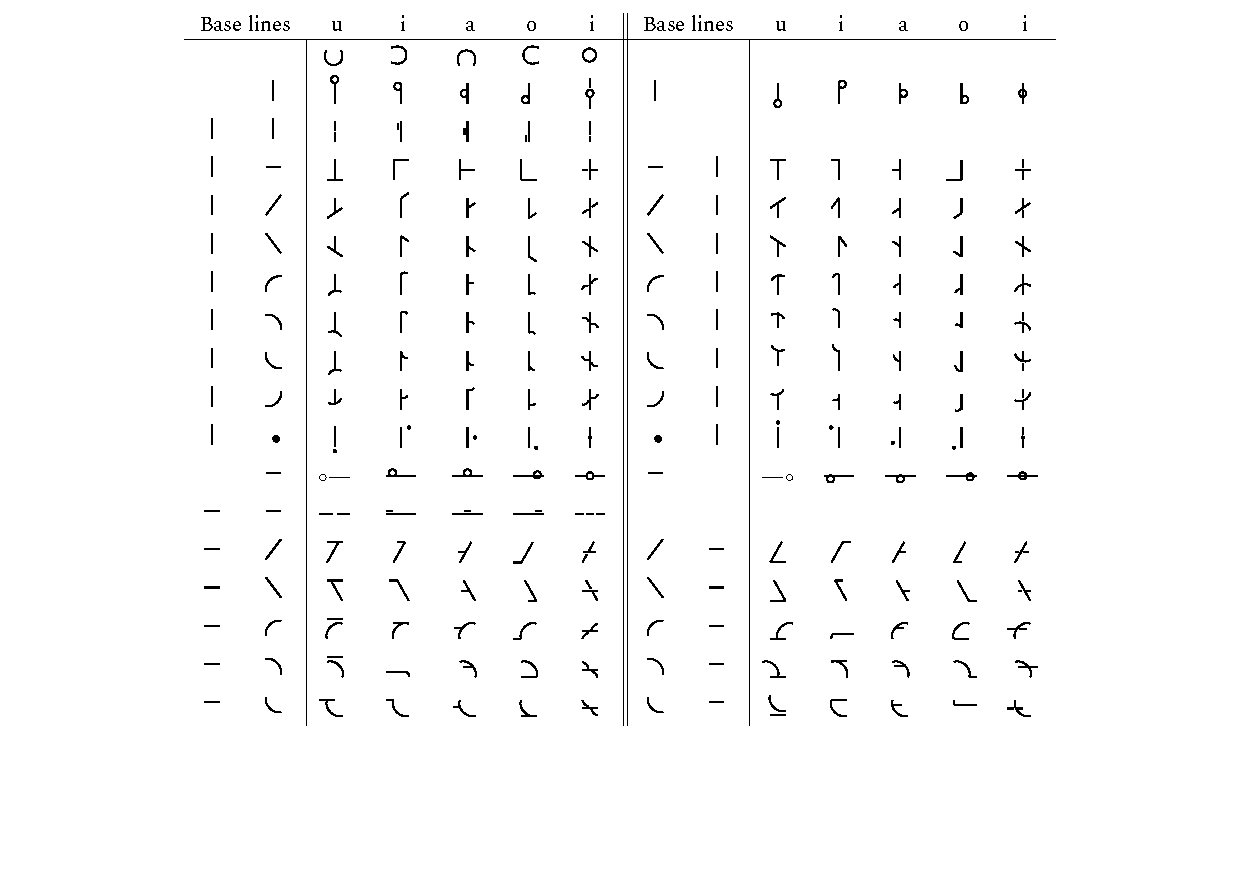
\includepdf[pages=1, pagecommand={}, width = 0.8\pagewidth, angle=90]{./TABEL.pdf}%LE-crop.pdf}
\pagebreak

\restoregeometry
\includepdf[pages=2, pagecommand={}, width = 0.8\pagewidth, angle=90]{./TABEL.pdf}%LE-crop.pdf}
\pagebreak
\newgeometry{rmargin=20pt, lmargin=50pt}

\includepdf[pages=3, pagecommand={}, width = 0.8\pagewidth, angle=90]{./TABEL.pdf}%LE-crop.pdf}

\restoregeometry
\section{Direction of reading -- {\small Stijn Janssens}}

Out of the roughly 6.500 languages worldwide, only 12 languages read right to left. The biggest among these is Arabic, with about 1,7 billion speakers. Preferred reading direction has to do with the materials on which the language was historically written, correlating with the technique used to write or carve letters. However, since LtR languages form the majority, and writing materials don’t form an obstacle anymore in our modern world, Atlan will use this reading direction as well. Nearly all human languages on earth are written in rows, stacked from top to bottom, and thus Atlan will do the same. This will also make it hospitable to digital environments and graphic design. Because the syllable glyphs can be read all at once, they could also be stacked in vertical columns, reading from top to bottom, for example when employed in calligraphy, or writing along pillars or vertical ridges. 

\section{Punctuation}
Atlan has minimal punctuation, only having dedicated symbols for a comma and a full stop, and spaces are the same as in any other orthography. A comma is notated as a small half circle which is open at the top:\comma symbolizing an ‘open’ continuation of the sentence, and the full stop is notated at as a half circle which is open at the bottom: \period , symbolizing a closed sentence. 
%Punt \DeclareStroke{(1.75, -2.5) to [bend left = 50] (5.75, -2.5)}
%Komma  \DeclareStroke{(1.75, -2.5) to [bend left = -50] (5.75, -2.5)}

Other punctuation will be marked by Atlan’s semantic atoms: question sentences start with the interrogative particle E, and so this eliminates the need for a question mark. Exclamative sentences start with the particle O, eliminating the need for an exclamation mark. Other examples would be ‘\&’ being ‘AN’ (‘and’), ‘\%’ being ‘EP.NO’ (‘per hundred’), ‘:’ being ‘I’ (‘relative clause’) etc. 

\section{Transliteration}
Atlan words will be transliterated into the Roman alphabet using the archetype letters U, I, A, O, E, P, T, K, M, N, S, F, L, J. Dots are used in between each syllable, in order to prevent confusion about where syllables are broken up, since this could create ambiguity in meaning. Dots in between two of the same consonants (eg. AK.KA) or vowels (e.g. KA.AK) are pronounced as a glottal stop or shwa, respectively (see chapter 2.2 and 2.3). 

Atlan’s syllables are all (C)V(C). Some loanwords or names, however, might have two or more consonants in a row within the same syllable. In such cases, the individual letter lines that exceed the CVC limit, will stand on their own next to the syllable glyph. The name ‘Stijn’, for example, will then become ‘S.TEJ.N’. 

\section{Numerals}

Atlan also has a numeric system distinct from the familiar arabic-numerals. They look like this:
\pagebreak

\setlength{\columnsep}{10pt}

\begin{multicols}{4}
\small

1   \numbr{1} 

2   \numbr{2}

3   \numbr{3}

4   \numbr{4}

5   \numbr{5}

6   \numbr{6}

7   \numbr{7}

8   \numbr{8}

9   \numbr{9}	

\columnbreak

10   \numbr{10}

20   \numbr{20}

30   \numbr{30}

40   \numbr{40}

50   \numbr{50}

60   \numbr{60}

70   \numbr{70}

80   \numbr{80}

90   \numbr{90}


\columnbreak

100   \numbr{100}

200   \numbr{200}

300   \numbr{300}

400   \numbr{400}

500   \numbr{500}

600   \numbr{600}

700   \numbr{700}

800   \numbr{800}

900   \numbr{900}


\columnbreak

1000   \numbr{1000}

2000   \numbr{2000}

3000   \numbr{3000}

4000   \numbr{4000}

5000   \numbr{5000}

6000   \numbr{6000}

7000   \numbr{7000}

8000   \numbr{8000}

9000   \numbr{9000}




\end{multicols}

The bottom right corner will be the first order of magnitude (below 10), the upper-right corner the second order (tens), the bottom-left corner the third (hundreds) and the top left the fourth (thousands). This way, when reading a single numeral, one would read from left to right and top to bottom, first the thousands, then the hundreds, then the tens and then the below tens, like for example the number 2023 (\numbr{2023}). An empty line is equal to zero (\numbr{0}), and having one of the corners empty but others with a number attached means that that order of magnitude is zero (such as the third order of magnitude in 2023). Decimals can be made by using a comma and adding a numeral behind it: in this case the orders of magnitude are flipped: one behind the comma is a tenth, two is a hundredth, three a thousandth and four a ten thousandth. For example, 2023,2023 would be \numbr{2023}◡\numbr{2023}. 

An added benefit of this numeral system, besides taking less space, is that addition could be more visually intuitive for some numbers: \numbr{1} plus \numbr{3} equals \numbr{4}, \numbr{2} plus \numbr{3} equals \numbr{5}, \numbr{1} plus \numbr{6} equals \numbr{7}. 

Atlan’s numeral system also allows for a duodecimal base notation, with the addition of unique numerals for 10 and 11: 

\vspace{0.2cm}
{\small
10 = \numbr{10}, 120 = (\numbr{120}), 1440 = (\numbr{1440}), 17280 = (\numbr{17280}) 

11 = \numbr{11}, 132 = (\numbr{132}), 1584 = (\numbr{1584}), 19008 = (\numbr{19008}) 
}
\vspace{0.2cm}

The added benefit of a duodecimal system is that certain fractions divisible by 2, 3, 4 and 6 are more straightforward to calculate by heart, whereas 10 can only be divided easily by 2 and 5. Another benefit is that it is more suited for many numerical systems, such as time divided into 60 seconds per 60 minutes per 24 hours, the twelve months and zodiac signs, as well as rotation being divided into 360 degrees.  

\pagebreak
\begin{wrapfigure}{r}{0.4\textwidth}
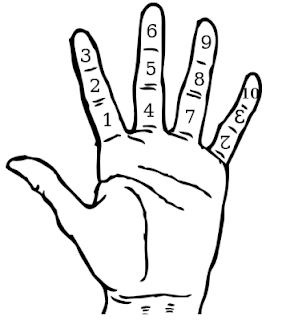
\includegraphics[scale=0.4]{./Images/Hand.jpeg}

	{\it \footnotesize Image taken from West (2015). }
\end{wrapfigure}

The duodecimal system can also be easily counted on a single hand, by using the thumb of the same hand as a pointer to count off the 3 finger segments in the 4 remaining fingers (see figure). Atlans number syllables fit this system as well: 1, 2 and 3 are ´IP´ \ip ´OP´ \op ´UP´ \up, since these all end in P they are grouped together on the first finger. 4, 5 and 6 are ´IK´ \raisebox{-0.5em}{\ik} , ´OK´ \raisebox{-0.5em}{\ok}, ´UK´ \raisebox{-0.5em}{\uk}, following again the same vowel pattern, but with K, grouping them on the second finger. Similarly, 6, 7, and 8 are ´UK´ \uk ´IM´ \im ´OM´ \om, and 9, 10, 11 are ´JI´ \ji ´JO´ \jo ´JU´ \ju. 

Currently, Atlan does not have a standardised system to clarify beforehand whether decimal or duodecimal numerals are used, other than to spot the usage of the numerals \numbr{10} and \numbr{11}. Frankly, current duodecimal systems in Arabic notation don´t have this either, but it could be easily stated verbally beforehand.  

 

\section{Mathematics -- {\small Stijn Janssens}}

Just as with punctuation, mathematical symbols can be approximated by semantic atoms. For example, plus + could be ‘AN’ \an (‘and’), minus - could be ´NE´ \ne (´negative´), divided by : could be ´EP´ \raisebox{-0.5em}{\ep} (´per´), equals = could be ´ME´ \raisebox{-0.3em}{\me} (´equal´). This way, speakers will not be required to learn many new mathematical symbols, but rather the glyphs could function as these, as well as carrying their own pronunciation and meaning. More complicated mathematical symbols or notations might need to be formalized and standardized by mathematicians, which might require more than one syllable. 




\section{Typography}



\noindent Since Atlan’s writing system is comprised of a set of basic lines, a great degree of artistic freedom is possible in creating different fonts and calligraphy styles to write the language. Atlan typography should make sure to remain faithful to the specific orientations of the different lines as to not cause confusion between them. Since any glyph contains a minimal amount of lines, usually two, typographic ornamentation can be added to glyphs without causing much confusion. Here we provide four examples of typographic variations on the word ‘Atlan’: a Times New Roman font, a {\it Comic Sans}-style font, Asian-style calligraphy and Arabic-style calligraphy.


\begin{center}

\includegraphics[scale=0.15]{./Images/Atlogos.jpeg}

{\footnotesize \it Figure 1: Atlan in different typographic styles.}
\end{center}
\section{Names, loanwords, and cartouches}

Words that denote certain names, such as personal names, placenames, names for institutions, as well as loanwords denoting certain culture-specific objects or concepts, like certain meals, for example, are incorporated into Atlan as phonetic approximations of these words in their source language. Because every possible syllable in Atlan already has its own designated semantic value, this could cause confusion, if the syllables are interpreted as Atlan words instead of loanwords. For this reason, names and loanwords always follow the following structure: 

\begin{itemize}
	\item denoting category, e.g.: 
		\begin{itemize}
			\item[] person \ej (EJ)
			\item[] place \lu (LU)
			\item[] town \tos (TOS)
			\item[] food \maj \kos (MAJ.KOS)
		\end{itemize}
	\item NA \na (name)
	\item phonetic approximation  

\end{itemize}

Using this formula, ‘Paris’ would become: ‘TOS.NA. PA.LI’ \cartouche{\tos \na \pa \li}, and ‘curry’ would become ‘MAJ.KOS. NA.KA.LI’ \cartouche{\maj \kos \na \ka \li}. If the conversational context makes it explicit enough that the subject matter concerns a loanword, and not a literal Atlan word, the markers denoting category + NA may be omitted for the sake of fluent speech.  

In (formal) typography, a cartouche may be employed to encircle the phonetic approximation in order to enhance intelligibility. Cartouches originate from Ancient Egyptian hieroglyphic orthography, where they were used to encircle the names of pharaohs (see Fig. 1) (Chrisholm, 1911).  

\begin{wrapfigure}{l}{0.4\textwidth}
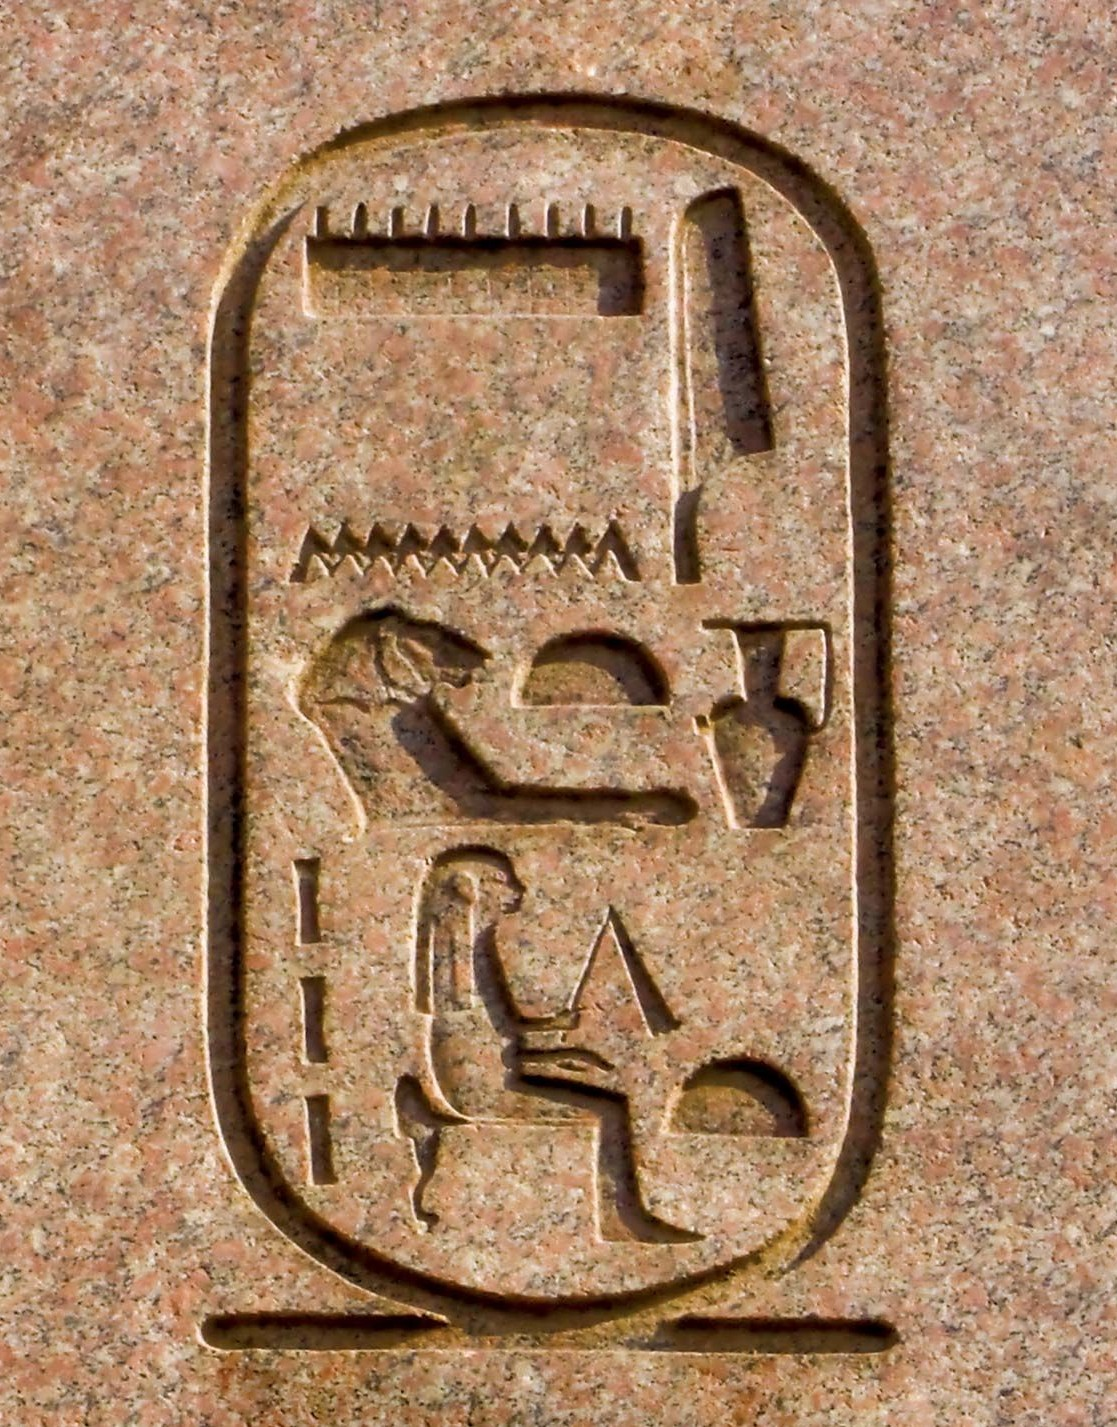
\includegraphics[scale=0.1]{./Images/Cartouche.jpeg}
	{\footnotesize \it Fig.1 Cartouche of Hapshepsut, one of the few female pharaohs in Egyptian history. She was often referred to androgynously because of a lack of feminine royal nomenclature (Graves-Brown, 2010). }

\end{wrapfigure}
 

The cartouche originates from the hieroglyphic ‘shen’, a stylised loop of a rope, which literally means ‘to encircle’, but had come to symbolise eternal protection. Therefore, it was also believed to have apotropaic powers (warding off evil). The word ‘cartouche’ comes from the French word for ‘paper bullet cartridge’, first applied when Napoleon’s soldiers encountered the frequently occurring glyph and noticed its resemblance to such cartridges (White, 2002). Interestingly, cartouches played an important role in deciphering Egyptian hieroglyphics. The early Egyptologist Thomas Young, following a suggestion from the decipherment scholar Jean-Jacques Barthélemy, compared the cartouches that appeared on the Rosetta Stone to the proper names that appeared in the Greek text (Robinson, 2009). This way, he was able to decipher the name ‘Ptolomy’ (Young, 1823). If Atlan were ever to become widely used, and inscriptions were made employing cartouches, perhaps the archaeologists of some distant future might employ them to decipher the script in the same manner that Young did. 

The 2001 conlang Toki Pona by the Canadian linguist Sonja Lang also employs cartouches in these contexts, for the same reason that Atlan does so (Lang, 2016). Just like in Toki Pona, Atlan’s cartouche shall be a simple oval circumscribing the name or loanword, without the additional straight line as used in Egyptian cartouches. One could object that employing a typographic element that derives from a specific cultural tradition, namely that of ancient Egypt, is in conflict with Atlan’s constraint of cultural neutrality. To this we object with the following justifications: the cartouche serves a practical function in preventing orthographic ambiguity; the Ancient Egyptian culture is currently extinct and thus does not advantage current day Egyptians over any other culture; the historical origin adds an extra layer of symbolism and cultural depth which in no way interferes with practical use; and frankly, we are of the opinion that it looks quite cool. 

As we will see in the next part, the glyphs can be made on the computer using \TeX\footnote{We will talk more of \TeX shortly.}. This also is true of cartouches. A cartouche can be made by simply saying \cartouche{name}. For example, the \TeX\ code  {\tt \symbol{92}cartouche\{Utrecht\}} produces \cartouche{Utrecht}\footnotemark  

\footnotetext{Utrecht = UT-LEK-T }

 


\section{On Dyslexia -- {\small Stijn Janssens}}

About 3 to 7 percent of the population has some form of dyslexia (Peterson \& Pennington, May 2012),(Kooij, 2013), however up to 20 percent of the population experiences some degree of its symptoms (National Institutes of Health, 2015). For Atlan’s writing system, this means that a minority group faces these problems, therefore not interfering with it’s universality / majority constraint. However, from the perspective of the world population, this still amounts to a significant group of people that might be disadvantaged by a writing system that is hostile to dyslexia. Atlan’s writing system has some aspects that work with and others that work against dyslectics.  

Within language psychology, different orthographies are classified by their orthographic depth. Shallow orthographies are mostly phonetical, encoding all the necessary information for pronunciation in a straightforward and consistent way. Deep / opaque orthographies are on the other end of the spectrum, often deviating from literal, phonetic spellings, or omitting certain phonemes from written language (Besner \& Smith, 1992). Examples of languages with shallow orthographies are Hindi, Spanish and Turkish, while examples of languages with deep orthographies are English, French and most extremely Tibetan (whose last spelling reform took place 800 years ago).  

Ideally, an IAL has an orthography that is as shallow as possible, making it more accessible for dyslectic people, as well as optimising learnability for non-dyslexics. In this regard, English is quite a poor IAL candidate. Because of great phonetic shifts and many etymological spellings (see chapter 8.2.0 on language variation), English orthography is highly inconsistent, which can be shown by pushing it to some quite absurd extremes. The word ‘church’ could hypothetically be spelled ‘tolot’, by combining the ‘t’ as pronounced in the word ‘picture’ with ‘olo’ as pronounced in ‘colonel’. The word ‘fish’ could be spelled ‘ghoti’, combining the ‘gh’ from ‘enough’, the ‘o’ from ‘women’ and the ‘ti’ from ‘nation’. The word ‘what’ could be spelled ‘oed’ by combining ‘o’ as in ‘one’ with ‘ed’ from ‘hacked’, and ‘why’ could be spelled ‘ho’, using the ‘ho’ from ‘choir’. Different spelling proposals have been suggested during the past centuries, however no major reforms have been established because of low public acceptance (Wolman, 2009). 

Because Atlan is spelled phonetically, it might be seen as having a shallow orthography. However, because of its syllabic nature, vowels are not directly notated but rather implied by the place of conjunction of consonant lines. Therefore technically speaking, vowels are notated, however they might require more focus and attention to be interpreted. More concerningly, many of Atlan’s glyphs have symmetrical counterparts, or are composed very similarly, only differing in orientation or place of conjunction. Since the Roman letters p, q, p and b are often confused, we might expect that such symmetries and similarities might also pose a problem for Atlan. A counterargument could be that the specific locations of line conjunction in Atlan is very regular and straightforward, only requiring readers to identify these relative positions in order to differentiate them from one another. Since Atlan does not have any fluent speakers at the time of writing, its actual effect on dyslexia can only be guessed. Therefore, we shall briefly discuss three example orthographies that share some similarities with Atlan, with respect to dyslexia. 

Most research has been done on alphabetic orthographies, most often English, this tendency is also known as {\it alphabetism}. Therefore, it is hard to come with concrete data on the effects of other types of writing systems on dyslexia. Hangul, a {\it featural}\ writing system used for writing Korean, has many letters that look alike, or are each other’s mirror image: ㄴ, ㄱ, ㅓ, ㅏ, ㅕ, ㅑ, ㅗ, ㅜ, ㅍ, ㅛ, ㅠ, ㅅ, ㅈ, ㅊ. Hangul’s orthography functions by combining letters into syllable blocks, therefore resulting in blocks that are sometimes barely distinguishable from one another at first glance, like 반 \& 번, and 본 \& 분. Surprisingly enough, many Koreans are unaware of the existence of dyslexia. A possible reason for this might be that Koreans read by identifying each syllable block all at once, rather than reading all the different letters within each block. Therefore, native speaking Koreans who learn to read as children might not experience any symptoms of dyslexia, because they learn to recognise many different syllable block combinations as single images, while always having the phonetic cues present within the block to verify if they read it right (jreidy17, 2014). This would foster a strong association between visual cues, pronunciation and meaning. Atlan might have the same benefit in children learning the language at an early age, where they might learn to recognise each glyph as an individual image, directly associating its pronunciation with it since this information is encoded in the glyph. Since each Atlan syllable glyph has a unique meaning assigned to it, this might even result in quasi-logographic reading, where people might recognise the word, its meaning and pronunciation from its visual shape. People who learn Atlan at a later age might not have this benefit and struggle more with learning the language, as they might keep trying to read each glyph letter for letter, making possible confusion more likely. 

The Inuktitut language of the Inuit people employs a writing system which, like Atlan’s writing system, might be classified as a featural syllabary, or an {\it abugida}. It was developed by Christian missionaries in the 19th century, and just like Atlan, it consists of basic geometric shapes and lines, with different orientations or symmetries indicating different vowels, e.g.: ᐱ = pi, ᐳ = pu, ᐸ = pa, ᐯ = pai. Research into dyslexia among Inuktitut speakers is scarce, but the small existing body of research suggests that such writing systems are not any more difficult to learn for children than other writing systems, and that they might even be easier to learn as a first writing system because of the clear parsing of syllables as linguistic units (Donovan \& Tulloch, 2022).  

The Amharic language of Ethiopia uses an abugida named ‘Fidel’. This writing system requires speakers to memorise many different basic shapes, some of which are very similar to one another, which are then systematically modified with small grapheme variations to indicate different vowels. E.g.: ጸ = ts’\"{a}, ጻ = ts’a, ጾ = ts’o, ደ = d\"{a}, ዳ = da, ዶ = do, ይ = d. Again, research is limited, but indicates that because of the nature of the writing system, glyph-naming is crucial for all other indicators of literacy (Mekonnen, 2023). When this type of writing system maximises legibility, this creates a positive feedback loop, but when it limits reading, it does the opposite, making overall legibility harder.  

\section{\TeX\ and Atlan -- {\small Jarno Smets}}
Atlan is precise when needed, but not forcingly rigid. Being all nitty-gritty is possible, but not demanded. Hence, the typesetting language \TeX\ \footnote{Or its modern forms \LaTeX\ and Lua\LaTeX, as used here.} is a great fit for this book, and for Atlan's writing system. Here I will quickly guide the reader through the uses of \TeX\ in this book.

First, there are our glyphs. They are hand-programmed in \TeX\ using Tikz. It was a strenuous effort, but worthwile. The glyphs are high-resolution, scaleable, and they also look the part. The usage is straightforward as well. 

To print any of the Atlan glyphs in \TeX\, you load in the package {\tt Atlan.sty}. Most glyphs are simply transliterations of syllables, with a backslash in front. E.g. \texttt{\symbol{92}mum} prints \mum. Some commands were already occupied, hence some of the commands are named differently, e.g. \texttt{\symbol{92}Atlanpi}, since simply \texttt{\symbol{92}pi} would print $\pi$. Next up, I plan to make a font that is available on other typesetting platforms. 

Then, our numeral glyphs rely on Lua\LaTeX\, a more potent version of \TeX. The command, again, is straightforward. You simply state \texttt{\\numbr\{<number>\footnotemark\}}. \footnotetext{Due to the nature of our numeric system, the biggest number you can fill in, is 9999.}  An example of the command: \texttt{\symbol{92}numbr\{321\}} produces \numbr{321}.  

Then, of course, this book is typeset in \TeX\. We could have made it easier for ourselves. But, typesetting with \TeX\ was worth the effort. We are proud of what we have made; both content- and appearance-wise.    







\chapter{Morphosyntax}
\Section{Unambiguous Syntax}{Jarno Smets}
\lettrine{A}{mbiguity} is of all times and places, and natural language is rife with it. {\it Goal}, {\it purple people eater}, {\it John trades with Mary}; these words and expressions can all be interpreted in multiple ways. Some despise ambiguity, while others wallow in it. Whatever one thinks of ambiguity, it is a part of natural languages. 

For our constructed language, we want to minimize ambiguity. This for the sake of clarity and communicability. Hence this essay.

In this essay, I will cover a specific type of ambiguity, namely {\it syntactic ambiguity}, also known as {\it structural ambiguity}. A sentence that can be interpreted in multiple ways due to its syntax, is structurally ambiguous.

My aim in this essay is twofold. First, I want to show why syntactic ambiguity is a problem, especially for the goals of our project. Then, I will propose a strategy to minimize this form of ambiguity, and argue for that strategy choice.

\section*{What is syntactic ambiguity?}

Syntactic ambiguity occurs when word-order gives rise to multiple interpretations (Oaks,2012, p.16) . The sentence \lq\lq I see the man with binoculars\rq\rq \phantom{} could be parsed (split into grammatical parts) in two ways:
\begin{center}
\begin{forest}
	for tree = {s sep = 0.5mm}
	[I see the man with binoculars[I see][the man with binoculars[the man][with binoculars]]]
\end{forest}

	\vspace{0.5cm}

	\begin{forest}
	[I see the man with binoculars[I][see the man with binoculars[see the man[see][the man]][with binoculars]]]
\end{forest}
\end{center}

\noindent {\footnotesize\it Figure 1: different syntax trees for \lq\lq I see the man with binoculars\rq\rq}
\vspace{0.1cm}

\noindent As we see in the above syntax trees, the difference in interpretation hinges on the (de)coupling of the words {\it man } and {\it with binoculars}. You could make {\it with binoculars} modify {\it man}. One could also modify {\it see} via {\it with binoculars}. The structure of the sentence doesn't give preference to one over the other.

For further illustration: one common type of syntactic ambiguity, is {\it scope ambiguity}. Scope ambiguity co-occurs mostly with logical operators such as quantifiers (for all, there exists), negation, and coordinators (and, or, but)\footnote{These are all operators in propositional logic. Quantifiers: $\forall $ = for all , $\exists $ there exists, $\neg$ = negation, \lq\lq not \rq\rq. $\wedge$ = and/but, $\vee$ = or.}. {\it Scope} is the part of a sentence over which such quantifier, negation, or coordinator ranges. Other instances of scope ambiguity are seen with modifiers, which I will briefly discuss below. Scope and scope ambiguity can best be explained by example: 

\begin{singlespace*}
\begin{center}
{\it (1) My cat is not grey or black}
\end{center}
\end{singlespace*}

\phantom{}\\
\noindent Two readings for (1): my cat is neither grey nor black, he is red, for example. Alternatively, my cat is not grey, but is black of colour. The scope for negation is ambiguous here. The {\it not} either or it has scope over {\it grey or black}, or it only has scope over {\it grey}, . 


Where lies the origin of such structurally ambiguous sentences? Yang (2014) discerns five major causes of structural ambiguity in English: 

\begin{itemize}
	\item[A] Negation scope 
	\item[B] Words with special syntactic functions
	\item[C] Improper abbreviation
	\item[D] Unclear word-characteristics
	\item[E] Unclear modifier-relations
\end{itemize}

\noindent We discussed an instance of A above already. With B, Yang refers to words that generate {\it subordinate clauses}; subsentences. These sentences could either be the object of the bigger sentence, or be a truly subordinate clause. E.g.: {\it The girls reported to me when they came.} Did the girls report to me after they arrived? Or did they report their time of arrival? it is unclear, due to the meaning of the word {\it when} . 

Now on to cause C Yang mentioned. {\it Improper abbreviation} is the improper shortening of a sentence. Again, think of the sentence {\it Mary trades cards with Joe}. I could have said {\it Mary trades cards together with Joe} if I wanted to convey that message. But I didn't; I left out the word {\it together}, making it ambiguous. 

Then, an example will elucidate cause D: {\it drinking water is unsafe}. Is {\it drinking} a verb in itself, or part of the larger phrase {\it drinking water}? The word characteristics for {\it drinking} are unclear. {\it Drinking} can either be seen as a verb, or as a noun together with {\it water}.  

Finally, cause E refers to a modifier. A {\it modifier} is a linguistic element that changes the meaning of another linguistic element. For example, {\it grey} modifies {\it dog}. With unclear modifier relations, it is not apparent which modifier modifies what. In the phrase {\it purple people eater}, it is unclear whether {\it purple} modifies {\it people}, or {\it eater}.    


\noindent I propose we bring these causes down to two. Firstly, structural ambiguity is caused by unclear semantic roles. A {\it semantic role} of a word or sentence-part is the role it plays in the meaning of the sentence. For example, the semantic role of {\it the grey dog} is the same in both sentences underneath:

\phantom{}

\begin{singlespace*}
	\begin{center}
	{\it (2) The cat attacked the grey dog}\\
	{\it The grey dog was attacked}
	\end{center}
\end{singlespace*}
\vspace{0.1cm}

\noindent In the example given above, {\it I see the man with binoculars}, the semantic role of {\it with binoculars} is indeterminate. Is {\it with binoculars} how I see the man? Or does the man have binoculars? it is precisely this indeterminacy that seems to generate the ambiguity.

The second cause I propose, is unclear word-grouping and unclear scope. To get rid of the ambiguity in phrases as {\it purple people eater}, or {\it lesbian vampire killer}, it needs to be specified which words modify which. 

\section*{The issue for Atlan}

In the previous part, I examined syntactic ambiguity. Now, why is this a problem for Atlan?. I will here propose three reasons for that goal. First, I will argue that structural ambiguity inhibits the parsing of language by computers. Computer-parsing could boost the spread of Atlan. Secondly, I will show that some forms of syntactic ambiguity would endanger the communicative function of our constructed language. Atlan should be a bridge between two languages. Syntactic ambiguity can make it more difficult for two speakers from different languages to communicate.  Lastly, I will argue that, in some high-stakes circumstances, syntactic ambiguity could be a great danger.

First of all, syntactic ambiguity is a problem for computers. Computers need a so-called {\it parser} to understand our language: The machines pick apart a sentence, in order to fully understand it (Schubert,2020). Syntactic ambiguity is a true roadblock for such parsing. Because syntactic ambiguity gives rise to multiple parsing options, a computer can't give a definite parsing of a syntactically ambiguous sentence. To circumvent, or to (partially) overcome it, multiple algorithms have been created. Yet it remains a difficult problem (Chowdhary, 2020, p.645).

For our constructed language, computer parsing and processing could be of help to the language learner. Translations would be more accurate, and practice materials can be generated more quickly. The presence of syntactic ambiguity is troubling for computers to analyze natural language.

Besides, structural ambiguity endangers universality. Since our language is intended as an auxiliary constructed language, people learn our constructed language as a {\it second language}. Hence, learners all approach our language from the perspective of their mother tongues. Now here lies the problem: different languages have interpret scope in different ways.

This has been shown, for example, in Scontras et al. (2017). This team of researchers found out that Mandarin lacks \textit{inverse scope}. Inverse scope can best be explained by an example: \lq\lq A badger dug every hole \rq\rq. In English, two readings are available for such sentence:

\begin{itemize}
	\item[]Surface scope - {\it There was one badger such that it dug every hole.}\\
		Inverse scope - {\it For every hole, there was a (different) badger that dug it.}
\end{itemize}
	
\noindent Scontras et al. found out that the inverse scope reading is simply not available in Mandarin Chinese. Furthermore, they found out this lack of inverse scope is found in the English of native Mandarin speakers. Another study showed similar results: Korean learners of English habitually preferred the surface-scope reading, and left the inverse-scope reading out (Seon \& Shin, 2022). 

So, when learning new languages, speakers have the tendency to bring their native scope-reading preferences with them. This endangers the communicative function of our conlang. If our constructed language has certain scope ambiguities in it, miscommunication can occur. Say you have speaker X, in whose language both scope-readings are available. She communicates such a scope-ambiguous sentence to speaker Y. X wants to bring across the inverse scope-reading. To speaker Y, {\it inverse} scope-readings are {\it not} available. Then X fails to bring across {\it her} wished interpretation of the sentence; a communicative error has occurred. Hence, structural ambiguity endangers the communicative clarity of our constructed language. 

Expanding further on communicative clarity: some contexts strictly demand that there be no ambiguity. Hazardous environments, such as nuclear power plants, weapon factories and the like, should communicate in a clear, unambiguous manner. Also law practice should be ridden of ambiguity. These are high-stake-environments. Any communication mistake could have far-stretching consequences. 

Say an English nuclear-power plant has the following instructions etched into an important control panel: 

\begin{center}
	{\it (3) In case of emergency: pull the horizontal striped lever} 
\end{center}

\noindent Now, there are two levers in the control room. One is a lever you pull from north to south, and it is marked with horizontal stripes. The other lever is horizontal, but has vertical stripes instead. Which lever do you pull? I hope this example makes it clear how dangerous syntactic ambiguity can be. 

Of course, this was a fabricated example. A real-life example, can be found in (Layman,1962):

\begin{singlespace*}
{\center  \it

	(4) Serbian subjects in the United States, shall enjoy
the rights which the ... laws grant ... to the subjects of the most favoured nation. 
}
\end{singlespace*}
\phantom{}\\

\noindent Example (4) elicits two interpretations: Serbian subjects who reside already in the United States enjoy the rights, or Serbian subjects, independent of where they remain, enjoy the rights when they are in the United States. This is syntactic ambiguity in law. Here it can have grave consequences for a large number of citizens.

With these few examples, I have shown why syntactic ambiguity is best left out in our constructed language. Firstly, it would make it hard for computers to parse our language. That while computers generally help to spread a language faster. Secondly, structural ambiguity in a language can cause miscommunication within a language. Not every language allows multiple scope readings, for example. Scope ambiguity can then lead to miscommunication in a language. Thirdly, syntactic ambiguity can be of real danger. It could cause communicative issues in high-stakes environments, such as infrastructure and law.  

It must be noted, however, that syntactic ambiguity is not only a {\it bad} phenomenon. It can also serve poetic and humorist endeavours. For example, the structurally ambiguous sentence

\begin{singlespace*}
	\begin{center}
		{\it (5) Time flies like an arrow; fruit flies like a banana}
	\end{center}
\end{singlespace*}

\noindent is undeniably witty\footnote{Found in (Cornish-Bowden, 2015).}. Does the fruit fly similar to a banana, or do fruit flies love a banana? The first part of (5) seems to prime the reader for the first reading.  

\section*{Minimizing syntactic ambiguity}

\noindent Now I will look at the efforts of other constructed language to minimize syntactic ambiguities. I will examine the benefits and downfalls of their approaches. From that examination, I will aim to distill the strategy for {\it our} constructed language to bring structural ambiguity to a minimum. 

One of the main origins of structural ambiguity is the distance between sentence-parts. In a structurally ambiguous sentence, it becomes unclear how the words are fit into phrases, and then how phrases fit in a sentence. For example, in the noun-phrase {\it purple people eater}, does {\it purple} belong to {\it people}, or to {\it eater}? Solving structural ambiguity is then making clear which words modify what , to only give one interpretation of a phrase or sentence.

The constructed language Lojban\footnote{Lojban [lo\textyogh ban] is a constructed language, created by a group of people wanting to improve another constructed language, {\it Loglan}. One of its spear points is having an ambiguous syntactic structure. Found on: https://mw.lojban.org/papri/Lojban, may 23rd, 2023.} indeed does this. It has two ways of specifying which words belong together. The first manner comes in the form of the structure word {\it bo}. \def\bo{{\it bo} } {\it Bo} enforces scope (The Lojban Reference Grammar, 2023). To see how, let's take the English sentence \lq\lq That is a big bug catcher\rq\rq.\phantom{} In English, you could interpret this either as a big catcher of bugs, or a catcher of big bugs. In Lojban, the word \bo makes this difference explicit:

\begin{center}
	{\center (6) That is a bug-catcher that is big.\\ {\it Ta barda miptera bo kavbu\footnote{{\it Ta} = \lq\lq That is\rq\rq, {\it barda} = \lq\lq big\rq\rq, {\it miptera} = \lq\lq bug\rq\rq, {\it kavbu} = \lq\lq catcher\rq\rq, and \bo is the structure word. English translation found in  (Jbovlaste: a lojban dictionary, 2023)}.}}

{\center (7) That is a catcher of big bugs. \\}
{\it Ta barda bo miptera kavbu.}
\end{center}
\vspace{0.1cm}

\noindent As you might have guessed from the above examples, the structure word \bo \lq\lq pulls\rq\rq two words together, to combine them. Since the combination of words is made explicit by \bo, ambiguity is resolved. 

There is a second way of coupling words in Lojban. The makers of Lojban decided to make rules for grouping, the so-called {\it brivla}. {\it Brivla} is an umbrella term for nouns, verbs, adjectives and adverbs (The Lojban Reference Grammar, 2023). The {\it left-grouping-rule} states that the two leftmost {\it brivla} are grouped together. So, the sentence {\it Ta barda miptera kavbu}, is automatically parsed equivalent to the second reading above (The Lojban Reference Grammar, 2023). 

It seems Lojban got structural ambiguity under control with these two restrains. What are the advantages and disadvantages of this approach?

As already mentioned above, the word-groupings are made explicit, effectively removing structural ambiguity from the language. This increases the clarity of Lojban, and thereby makes the language more universal. There are some downsides however. As we saw above, some scope readings are not even available in the mother-tongue of some speakers. The left-grouping rule described above could enforce a reading upon the language learner, which the language learner is far from familiar with. Lojban then might sometimes give rise to miscommunications. 

\catcode`\_=11
Another constructed language with the intent of minimizing (syntactic) ambiguity, is {\it Ithkuil}. Ithkuil marks semantic roles explicitly in noun cases (Ithkuil, Case Morphology, 2023). This is relatively similar to German, where the case {\it der} usually marks the (male) subject of the sentence, or {\it des} marks the possessor. Ithkuil has more cases, including the ones we all know (subject, object, possessor, dative). Examples are {\it instrument}, {\it force}, {\it agent}, and much more\footnote{Readers interested in more should visit Ithkuil's website: http://www.ithkuil.net/newithkuil_04_case.htm.}. 


Ithkuil specifies the exact case of every noun. Due to that, it is clear which word plays what role in a sentence. In {\it purple people eater}, for example, {\it eater} could be nominative, while {\it purple people} would be marked as accusative. In that way, ambiguity is brought down to a minimum. However, there is one big downside to this approach: it is too complex. Ithkuil is very complex, and hard to learn. Even the creator, John Quijada, can't speak it fluently (Foer, 2023). Thus, the ubiquitous presence of cases seems to do more harm than good; it eliminates ambiguity, but at the cost of learning-ease and fluency.

We have seen how Ithkuil and Lojban deal with syntactic ambiguity. Taking this in account, how will Atlan deal with it?

A feature of Lojban was the explicit word-coupling with the structure word \bo. The word directly made clear what words formed a separate noun-phrase. However, it is an extra word to remember. We believe it is a better idea to couple words in the most direct sense of the word: literally connect them to each other. This is a familiar feature of, for example, Dutch: {\it grijze hondentemmer} (grey hound-tamer) versus {\it grijze-honden temmer}. Both in English and Dutch, the words \lq\lq dog \rq\rq and \lq\lq tamer \rq\rq are joined to indicate that they belong together. In speech, words that should be separated, are separated by a pause. 

Now, what about scope ambiguity? For negation, for example, we will include two types: sentential and predicate negation. Sentential negation is a form of negation that spans over a whole sentence. For this we put NE in front of the sentence. E.g. {\it I have {\bf not} been to school today}. Predicate negation on the other hand, only spans over a predicate. For this we put NE in front of the predicate (or noun). For example, {\it I'm very {\bf un}happy at the moment.} This would fix negation scope ambiguity. Take the aforementioned example {\it my cat is not grey or black}. The two readings can be separated using the distinction between types of negation:

\begin{center}
	{\it (8) My cat is ungrey or black\\ it is not the case that my cat is grey or black}
\end{center}


\noindent The sentential negation will take the form of a distinct particle, whereas the predicate negation will be an affix. This has the following reasons. Sentential negation spans over a whole sentence. To make it immediately apparent that a sentence is negated, it would be convenient to have a loose particle to place at the beginning of a sentence. Predicate-negation occurs within a sentence, and binds to predicates. Hence, it will be an prefix, connected to the predicate it negates.  

This approach to negation doesn't make it more difficult to learn. Most languages are familiar with it: th most common types of negation are negative particles, and affixes (Martin et al., 2005, p. 454) Even if, for a learner's mother-tongue, there is a mismatch between negation type (sentential and negation) and form (particle and affix), the forms are very likely familiar. This will very likely make our approach to negation somewhat more intuitive for a language learner. Moreover, predicate negation is present in a majority of languages (Martin et al., 2005, p.467).

But what about scope ambiguity outside of negation? E.g. {\it The dog or the cat and the bird made a mess}. Here, we appeal to operator strength from Classical Logic. Negation comes first. Then comes conjunction (\lq\lq and\rq\rq). Last comes disjunction (\lq\lq or\rq\rq) (O'Donnell et al., 2007, p.120)\footnote{After that comes the conditional (\lq\lq if...then\rq\rq, $\rightarrow$) and the bi-conditional (\lq\lq if and only if \rq\rq, $\leftrightarrow$). As far as I can tell, they don't seem to generate syntactic ambiguity, hence I leave them unmentioned here.}. In the above example, the sentence is read as: (the dog or the cat) and (the bird) made a mess. That the bird made a mess, is certain. Whether the dog or the cat made a mess is uncertain.



Now it is worth noting a few {\it caveats} about my approach. Firstly, I reasoned mostly from syntactic ambiguities in English and Dutch. This could leave room in my solutions for syntactic ambiguities not thought of by me. Hence, I talked primarily of {\it minimizing} syntactic ambiguity. Besides, it is worth noting that context will disambiguate as well. I have mostly examined structurally ambiguous phrases and sentences in isolation. Some of those phrases or sentences would not be as ambiguous in context.  


In this essay, I have shown two things. First, I argued that syntactic ambiguity should be avoided when constructing a language. This because syntactic ambiguity troubles computers, endangers communicative function, and  can be potentially harmful. 

Secondly, I have proposed several general recommendations for battling syntactic ambiguity. This I distilled from previous attempts at constructing structurally unambiguous languages, such as Lojbans and Ithkuil . Lojban made its structure clear, but had a redundant syntax rule. Ithkuil explicitly specified the semantic role of each word, but became extremely hard to learn and speak as a consequence. 

Atlan won't be as specific as Ithkuil or Lojban. It is a balance we need to find between preciseness and learnability. Both Ithkuil and Lojban are extremely precise, but sacrifice learnability. I am confident that Atlan will find a good balance, and that the learner will profit from that. 



\chapter{Our Ontology -- {\small Stijn Janssens}}%%Introduction

The goal of this chapter is to expound on the ontology of the language, which concerns its semantics and syntactical inventory. I will achieve this by discussing the literature on various attempts and classifications proposed within the topics, and then dividing all linguistic meaning into its irreducible, unambiguous and unique atomic components, as to respect constraint 2 (unambiguity). It will use some principles of natural bifurcation of meaning (chapter 5.1.2), and built off of the universal substratum of phenomenology and qualia (chapter 5.2 and 5.3). It will also be linguistically grounded in the culturally universal basic elements of human life (chapter 5.4).


\section{Parsimony in semantics}

\noindent {\it Oligosynthesis}


Besides constraint 1 (cultural neutrality), which will be discussed in chapter 5.4, Atlan’s lexicon has to follow constraint 2 (unambiguity) and 3 (parsimony), which will be discussed in this section. Ideally, the language should contain as little basic words as possible, as to reduce the time required to learn the language. Therefore, it should be sparse with its words, only adding new words when these carry a meaning that is not already covered by another word. Complex concepts should not get their own separate words, for this would add an inestimably large number of extra words, but rather be composed of more simple and universal words that constitute its meaning. Atlan shall achieve this by using a semantic system that is oligosynthetic, meaning that it has a very limited number of semantic atoms (\textit{oligo}  = few), from which more complex meaning is built by combining different atoms (\textit{synthesis}  = combining). Each semantic atom (or ‘root’) shall be covered by a unique one-syllable word. Atlan syllables can take four shapes (C = some consonant, V = some vowel): V, CV, VC, CVC. This is abbreviated to (C)V(C). There are 9 consonants and 5 vowels in its phonetic inventory, yielding a total of 5 + 5x9 + 5x9 + 5x9x9 = 500 possible combinations, however all syllables ending in \textit{-ij} cannot be sufficiently distinguished by ear from those ending in \textit{-i}, so all (-) \textit{ij} will not be included. This leaves a total number of 490, and thus the challenge posed in this chapter is that of reducing all meaning to 490 atoms or a combination of these.  

The term \textit{oligosynthetic} was first coined by the linguist Benjamin Lee Whorf and is defined as having at most a few hundred-word roots. However, this seems to be extremely rare among natural languages. A possible example might be the Kalam language of the Highlands of New Guinea (Pawley A. , 1993). Two other languages previously regarded as oligosynthetic by Whorf are the Aztec language Nahuatl and the Native American language Blackfoot, but these are now commonly classified as polysynthetic (using many roots to synthesise more complicated meaning). Oligosynthesis is more popular among constructed languages, such as Sona, Ro, aUI, Ygyde and Kali-sise (FrathWiki, Oligosynthetic language, n.d.). These all have different numbers of semantic primes and methods of synthesising them, but they commonly have the following problems (Watson, n.d.): 

\begin{itemize}
\item [I.] Complicated combinatory systems  

\item[II.] Unclear word-parsing  

\item[III.]Vagueness of composite meaning 
\end{itemize}

Atlan will overcome problem I by using an extremely basic manner of combinatory synthesis: the most semantically essential prime comes first and is followed by primes that hierarchically specify the meaning of the word. Grammatical functions always come in front of the semantic root as prefixes (except for the plural1), and semantic specifications are appended as suffixes.  

Atlan words composition:  

\begin{center}
{grammatical.function –  main.semantic.root – semantic.specification – plural} 
\end{center}

 

This will also solve problem II, because syllables can be recognised to be semantic when they are CVC, and grammatical otherwise. This way, grammatical syllables are easily distinguished from semantic ones. It is therefore always audibly clear where a word begins and ends. In written text this is aided by the fact that in Atlan’s own writing system, CV and VC syllables always consist of a small circle attached to a line, while CVC syllables are always two lines connected to each other.  

The 5 V syllables will be restricted to mood-markers and general sentence structuring, because of the onomatopoeic quality of these basic vocal sounds. These, however, can also be used grammatically to modify the meaning of nouns, verbs and pronouns, for example to turn ´here´ into ´where?´.  
\begin{itemize}
\item    Exclamative (prosody), imperative, vocative = o  

\item    Interrogative (question, prosody) = e  

\item    Stress marker (prosody) = a + stress 

\item    Relative clause = i (+ pronoun) 

\item    Subjunctive (wish) = u 
\end{itemize}

 

The 89 CV, VC syllables will be mostly restricted to morphological and abstract functions, indicating grammatical, syntactical or logical functions and relationships between words. Logical functions will be derived from the logical operators of predicate logic and possible worlds semantics (Priest, 2011), and grammatical functions are derived from the Universal Networking Language (UNL) (Portal, sd), and syntax-semantically reduced where possible (see chapter 6.2). UNL was initiated by the United Nations University in 1996 and continued by the international non-profit organisation UNDL from 2001 onwards. Its goal is to function as a formalised pivot language between natural language and interlingual machine translation, therefore having formalised all grammatical functions, together with a large-scale ontology of all concepts contained within all its source languages (Universal Networking Language Portal, n.d.). Atlan does not use the latter, however, because it would break constraint 3, parsimony. 	

The remaining 396 CVC syllables will cover the semantic primes, and these will be systematically selected and ordered in the remainder of the current chapter and chapter 3 and 4. Because Atlan’s writing system is syllabic, and each syllable has a fixed semantic value assigned to it, individual glyphs can be read both phonetically as well as ideographically/logographically. This would allow for it to be a kind of interlingual orthography. 

Problem III, that of vagueness of composite meaning, will be tackled in several ways. Most importantly, some of the most universal ‘semantic molecules’ (see chapter 3) will have their own assigned syllable. These molecules are definitions that could be reduced to more fundamental atoms but are often used to build more complex meanings, therefore being condensed into a molecule as to prevent unnecessary complexity of compound words. However, this is not an all-encompassing solution for words that have very specific and context derived definitions. 

{\it Circumlocution} is the phenomenon where concepts which do not have a specific word for them in a language are described by giving a circuitous description of the intended meaning. An example of this in English would be ‘the day after tomorrow’. Atlan will never be able to fully eliminate some forms of circumlocution in its lexicon, mainly because of it being an oligosynthetic language. However, confusion around these instanced can be minimalised in the following ways.  

A standardized set of compound definitions can aid speakers by being a guideline to using compound words. Someone who learns the language, would have to learn the 490 semantic primes, and then be familiarized with some standardized compound words. Because the meaning of the compound word will be derived from the syllables it contains, learning these compound words will be intuitive and require less mnemonic effort than learning a completely new word would. This way, when a speaker encounters a word they have never heard before, they will be able to derive, or at least estimate the intended meaning just by recognizing its syllables.

Additionally, neologisms could be created during improvised language use, as a sort of generative etymology, and be directly perceived by the listener, possibly allowing for freer linguistic cultural- and self-expression. Finally, some compound words will be systematically constructed in a taxonomical fashion, when the word’s definition allows for this, such as is the case for all living creatures. Each compound word is sorted along the axis of importance, with the most fundamental semantic prime in front, and followed by other primes that hierarchically add layers of semantic precision. This creates a universal logic in the composition of compound words that allows one to identify the ontological category in which the word falls and refine the definition by the refining descriptors appended to it, as if ‘zooming in’ with a semantic lens.


\noindent{\it Taxonomy}
\vspace{0.3cm}

\begin{center}
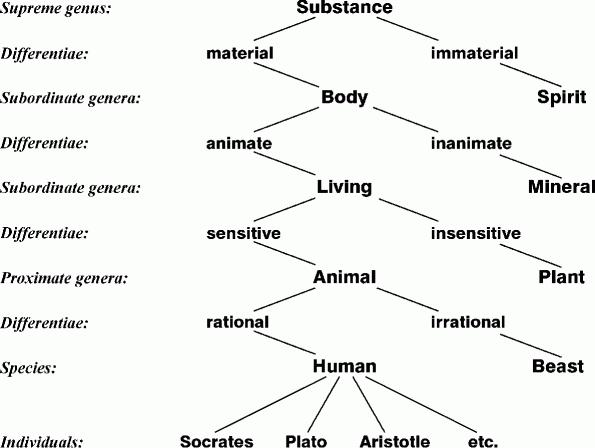
\includegraphics[scale=0.5]{./Images/tree.jpeg}

{\footnotesize \it Tree of Porphyry, taken from Cohen (2007)}
\end{center}

\noindent Many philosophical constructed languages that came before Atlan suggested or employed a so-called taxonomical ontology. Many of these are inspired by a diagram invented by the 3rd century Neoplatonist Porphyry when explaining Aristotle’s Categories (Porphyry, 300), called the Porphyrian tree (Franklin, 1986). In the Categories, Aristotle outlines a broad ontology of human apprehension, classifying everything that can be the subject or predicate of a statement into 10 categories: substance, quantity, quality, relation, place, time, position, state, action, affection (Aristoteles, 40). The Porphyrian tree (shown below) shows how a human falls into these categories, by showing different bifurcations from the first five categories (Cohen, 2007): 

Before Aristotle, similar ontological categorisations were made by the Vaiseshika school (Padārtha) (Stanford University, 2019) and the Stoic school, and after him numerous other thinkers, including Plotinus (430, 2019), Kant (Categories) (1781, 1998), Hegel  (1812, 1975), Peirce (1867), Husserl (1900, 1993) and Whitehead (categorial scheme) (1929, 2010). Not to mention folk ontologies, such as the Bantu nominal classes (Bleek, 1862–69) and the common distinction between animate and inanimate. All of these mostly were not taxonomical, however, and have been discussed extensively, but it is not the purpose of this paper to further investigate these discourses.  

There is, however, one specific notion within these categorisations which Atlan will incorporate, namely that of the {\it triadic categorisation} of Being. In Hegel, this comprises 1) Being (mind, consciousness, sensation), 2) Essence (Other, duality) and 3) Notion (synthesis, reference). In Peirce, these equate to Firstness (Quality, feeling, consciousness), Secondness (Reaction) and Thirdness (Meaning, representation). Atlan incorporates this through three degrees of removing from the speaking subject (see chapter 6.2). The first degree can be combined with the semantic prime for ‘person’ (´EJ´ \ej) to mean ‘I’ (´EJ.AM´ \ej \am), the second degree to mean ‘you’ (EJ.UN \ej \un) and the third to mean ‘he / she / they’ (´EJ.AJ´ \ej \aj), as well as other primes like place, time and demonstratives. 

A more explicit taxonomical ontology makes use of a so-called hierarchical classification. The idea of a ‘perfect’ or philosophical language was a popular idea during the enlightenment, being discussed by Bacon, Descartes, and Newton as a part of a widespread desire for a language that does not confuse the speaker’s understanding of reality or distort the natural order present in it (Eco, 1994, pp. 209-227).2 

The core idea of such a language is that it would build its words by adding different letters for every hierarchy of meaning. This way, related words would sound similar. There is, however, always a necessary degree of arbitrariness to such a system, since the arbitrary choice has to be made of what categories are specified by adding a limited set of different letters. These would have to be made from scratch, not based on previous languages, as to avoid confusion caused by natural language. These languages are known as a priori, and Atlan will be a priori as well, even though its contents are sourced from data from many natural languages but recombined in an attempt to circumvent natural language confusion.  

The first serious attempts at this ideal were made by George Dalgarno in his {\it Ars signorum} (1661, 1968) and John Wilkins in his \textit{Essay Towards a Real Character and a Philosophical Language} (1668, 1968). Initially, the two collaborated on a philosophical oligosynthetic language, but they couldn’t agree on whether to make the taxonomy encyclopaedic or build compound words from a small set of primes. Wilkins published his own version based on the former and Dalgarno the latter. Dalgarno’s language sadly never caught on, perhaps because the explanation of the linguistic working of the language was shrouded in philosophy which explained the structure \footnote{We hope this is not the case for this book as well}. 

Wilkin’s language found a bit more recognition, being originally taken seriously by the Royal Society, with an attempt to finish the language after his death by a designated committee. It too, however, slowly lost interest in people and descended into oblivion  (FrathWiki, Ars Signorum, n.d.). Its taxonomical classification was structured to encompass every animal, plant, mineral and artifact. He achieved this by setting up an ingenious taxonomical tree to indicate the relations and bifurcations of meaning, along with a system of hierarchically adding vowels and consonants to specify differences and species within different categories. 

Wilkins regarded the language presented in his essay as just a draft, although he provides 2,030 different primitives, as well as a 15,000-word list for different English words but admits that it should be worked out by different teams of scientists to work out different concepts within their respective disciplines. His collaboration with the Royal Society was largely part of that attempt. Later on, Wilkin’s taxonomy went on to inspire Roget’s Thesaurus (1805) and later on Diderot and d’Alembert’s Encyclopaedia (1759).  

The idea was met with a lot of criticism as well. Voltaire criticised the optimism of the people attempting to create such a language in the form of the character Dr. Pangloss in his satire \textit{Candide} (1759, 1963). Jorge Luis Borges wrote an essay criticising taxonomical categorisations in general and Wilkin’s language specifically (1942) in which he mocks different instances of arbitrary classification by mentioning a fictional Chinese taxonomy called the \textit{Celestial Emporium of Benevolent Knowledge}. This list contains some very culture-specific, arbitrary and absurd categories such as ‘those belonging to the Emperor’, ‘those that have just broken the vase’ and ‘those that from afar look like flies’. This criticism seems like a bit of a stretch, because Wilkins put in a systematic effort to make a coherent classification, and this is not as arbitrary or absurd as Borges’ fictional classification. The linguist George Lakoff supports this claim by stating that many non-western cultures use classifications similar to European ones (Lakoff, 1987). Borges does point out that a successful execution of the idea could in theory have many benefits: ‘‘Mauthner points out that children would be able to learn this language without knowing it be artificial; afterwards, at school, they would discover it being an universal code and a secret encyclopaedia’’ (Blevins, n.d.). 

Foucault was inspired by Borges’ essay to write his book \textit{The Order of Things} (1966, 2010, p. preface) in which he analyses the social grounding of epistemic assumptions. He argues that implicit norms within intellectual communities determine thought and influence which topics are researched, and which are not, and how the established bias influences the interpretation of the data that is found. These assumptions and norms are bound to cultural and historic settings, and periodically go through reforms as a result of paradigm shifts. This is a strong blow to the aspiration of a universal classification of the universe. Borges claims that this is because: ‘‘we do not know what sort of thing the universe is’’. Metaphysicians and phenomenologists might differ on this, however, as will be discussed in chapter 3 of this essay.  

Besides this, Wilkins’ system has the disadvantage of only having a limited number of differences and species that can be specified because of the limited phonology. Atlan will be more similar to Dalgarno’s language, in that it will not drive its words through a hierarchical process of taxonomy, but rather by combining primes at will, allowing for exponentially more semantic combinations than are possible in Wilkin’s system. 

Another problem of Wilkin’s language is that words with similar meanings have very similar pronunciations, to the point of confusion. Modern information theory warns of this (Norman, n.d.), and Eco even identified that Wilkins himself made such a mistake, confusing {\it Gade} (barley) for {\it Gape} (tulip) (1994, p. 249). This would hinder the language’s intelligibility when mishearing can easily change important nuances in definition, as well as making is harder to speak fluently, because any speaker would have to work through tables and flowcharts in their minds while simultaneously talking, without making any mistakes. The language would also be very intolerant of subtle shifts in pronunciation and phrasing that tend to occur naturally within languages over time, because this would cause the whole encyclopaedic house of cards to come crashing down. 

Atlan will not have this problem, because its semantic primes are syllables instead of phonemes, and Atlan’s phonemic inventory is built to accommodate variation in phonetic approximation and sound shifts within its 14 archetype letters, without causing confusion or ambiguity. 

The philosopher Deleuze and psychoanalyst Guatarri proposed an alternative to arborescent (tree-like, hierarchical) epistemic networks like employed by Wilkins and Dalgarno, namely that of a {\it rhizome}, an analogy with a decentralised plant root network (1980, 2019). Such a model does account for bifurcations and conceptual relatedness but is more modal and allows for more complex interlinking than mere hierarchy. It would also fit the philosopher Quine’s idea of an interrelated epistemic ‘web of beliefs’ (Ney, 2014), as well as Wittgenstein’s claim that concepts are not clearly delineated, but rather surrounded by a ‘corona’ of associated concepts (1953, 2010, p. p. 181). 

Because of this, the main ontology seems to be better off using a combinatory system, which would allow for endless recombination and web-like relationships between similar words. This however doesn’t mean arborescent taxonomy should be completely abandoned. The most relevant modern case of taxonomical classification is that of natural species, although individual species don’t have clear demarcations and are loosely defined by their ability to produce fertile offspring (Nature Publishing Group, n.d.). Genetic diversification happened through bifurcation, known as {\it speciation}. The reverse, different species merging into one through hybridisation, called {\it despeciation}, does sometimes occur (including among early hominins), but is exceedingly rarer (Junior, 2018). Because of this, the evolutionary tree of life is primarily arborescent. 

Modern biological taxonomy employs the following hierarchical classification: life – domain – kingdom – phylum – class – order – family – genus – species (Biology Dictionary, 2017). Atlan’s biological lexicon is constructed along this framework, using semantic primes to describe different bifurcations, inspired by the Latin etymologies employed in binomial nomenclature (a hangover from Latin being the academic {\it lingua franca}). These binomial nomenclatures only mention the genus and species names of an organism, and words to designate species can re-occur in other genera to identify other species, adding to the parsimony of terms required to name all creatures within this system. Atlan shall have separate primes for the categories: \textit{virus, bacteria, archaea, plants, amoebas, fungi, animals.} In chapter 4 of this essay, a few culturally universal animal terms are identified, and these will be reduced to: \textit{mammal, fish, bird, worm, reptilian, insect.} Other animals could be reduced to their descriptions: sponges could be designated as foam-animals, starfishes to star-animals, snakes to legless-reptiles, amphibians to mucus-reptiles, molluscs to shell-animals, jellyfish to mucus-animals etc.  

Chemical molecules could be named by formalising a translation of the IUPAC nomenclature of organic chemistry from the originally Greek roots (IUPAC, 2021). Just like Wilkin’s language, Atlan will be dependent on scientists and specialists of different kinds of professions to add formalisations of their respective jargon nomenclatures to the lexicon in order to fully flesh out its lexicon. 

The reason why such a systematic description of reality claiming to be universal might be problematic, could be that it claims to have an objective image of reality, while all human thought, individual or collective, will always be fundamentally sourced from subjective experience. The philosopher Thomas Nagel described this by saying that there is no \textit{view from nowhere}\ (1989), while such a taxonomy appears to claim this anyway. The fact is that human concepts always have a necessary degree of arbitrariness because of the limited resolution of our conceptual boundaries. A taxonomical ontology implies the possibility of grasping some fundamental reductionist principle inherent to reality, while failing to see that many human concepts are emergent phenomena. The linguistic concept of an ‘organism’ cannot be reduced to a collection of organic molecules, because it is their complicated interplay that generates the multiple properties that pertain to an emergent system of self-preservation that humans call a single organism (Brigandt \& Love., 2017). On a microscopic level however, the clear boundaries of any single individual become fuzzy. It is because human life does not generally take place within a microscopic paradigm, that our concepts don’t have this level of detail. Reality is never described objectively, but always relative to the individual(s) observing and describing their reality. Humans appear to be ‘at the centre’ of their own language and understanding of reality. 

\section{The anthropocentricity of language}

Language and ontology are strongly entwined with one another: an ontological system is dependent on the words available to name its parts, and likewise a language is built from the set of concepts, relations, abstractions and ‘things’ that are captured by its lexicon  (Moltmann, 2017) (Boucon, 2019). Though by far not being the only elaboration on this idea, the Sapir-Whorf hypothesis is the most well-known inference that has been drawn from it. In short, this idea postulates that the range and limits of a person’s thought are determined by the language they speak. The strong version of this claim, linguistic relativism contends that all of human thought is fundamentally determined by language (linguistic determinism), resulting in some thoughts being lost and modified through translation or even untranslatable. It treats language as a fixed set of cognitive tools that acts as a constraint on the individual. This view, however, doesn’t enjoy a scholarly consensus (Whorf, 1956).  

However, this conception of language seems to be monolithic and extra personal instead of dynamic and dependant on individuals and their fluid interactions. It is challenged when presented with the fact that people within the same language can have vastly different ontologies, philosophies and vocabularies, depending on their individual personalities, interests and social environment, and the fact that individual people can learn multiple different languages and express their thoughts through them, nonetheless. Multilingualism is, however, noted to create within an individual, multiple linguistic ‘personæ’ for the different spoken languages, where one’s way of formulating thoughts and uttered sentences are altered by the individual characteristics of the different languages  (Pavlenko, 2006). 

Perhaps the influence that language has on the thoughts of its speaker can be likened to how putting on different glasses can alter one’s perception but does not change the fundamental scene being perceived through them. Sunglasses block out UV light, tinted glasses block out certain colours, different lenses shift the focus to what is near and other to what is far etc.: they all suppress some elements and amplify others, but they never change the basic composition of what is being perceived (if we discount virtual reality glasses). 

Using this metaphor, the purpose of Atlan is somewhat similar to being a clear, untainted, undeformed, unbiased pair of linguistic glasses, for as far as this is possible. Every single person’s eyes are different, and the glasses of their native language might be more or less similar to Atlan’s. The question then becomes: what constitutes this clear human experience that becomes tainted by language?  

First, we must realise that language itself is ontologically dependant on the total sum of living speakers. A dead, forgotten or undeciphered language cannot be said to currently exist in the same way that a living language like English exists. It might be revived in the future through the reconstruction of its linguistic information, but it only comes back into being when living humans are again able to read, write or speak the language. Furthermore, Wittgenstein’s private language argument states that a language is a fundamentally social thing, and that a purely personal language is therefore by definition impossible (1953, 2010, pp. \S 243-271). Language is a complicated system of communicating all kinds of mental information, like thoughts, feelings, intentions, physical data \&c., for all kinds of different purposes, like cooperation, social bonding, problem solving . In individual growing up in solitude or alongside animals never has the need nor possibility to learn and use a language, because there are no other humans around to converse with. After having passed the critical period of language acquisition without ever having learned a human language, an individual will never again be able to do so later in life (Robson, 2002).  

Therefore, language is an inherently human thing, that emerged from the transferring of information from one person’s individual experience to another’s. Phenomenal cues, like the sound of words, the rhythm of speech, facial expressions and gestures are used as an interpersonal bridge between the private mental worlds of the separate individuals. Someone can both hear themself talking, as well as someone else: language exists in a shared phenomenal space, whereas inner thought is private. Language then becomes a highly codified system of phenomenal metaphors. The sound of a specific word is not the same as the information it codifies, but is consistently associated with the referred phenomenon, in the form of an abstracted ‘concept’. 

Atlan should thus have an ontology that is built off the subjective human experience, when regarded in a social context and in direct contact with its physical environment. This immediately brings a degree of anthropocentricity with it, because words relating to the human psyche, body, daily life, social environment etc. will be given higher priority than the myriad of concepts and jargon within specialized disciplines that are less directly related to the everyday human experience. Moreover, humans should be able to think, talk and understand fluidly in a language, and not be required to consciously perform complicated linguistic computations within their heads while using the language. 

 

\section{Phenomenological ontology and qualia} 

Subjective experience is ultimately prior to any claim, idea, observation, connection \&c that can be communicated about reality. Anything in the world has to first present itself to us humans through phenomenal, subjective experience, before we can abstract it and understand it as an ‘objective’ phenomenon. However, the mainstream scientific metaphysical framework has, up to now, consistently been materialist, physicalist and reductionist. When it does acknowledge the existence of mind, it often does so in greatly unsatisfactory manner by employing some version of dualism, with the mind being metaphysically separate from the physical, but somehow miraculously still having epistemological and sensory access to it and the ability to manipulate it (moving one’s body at will) and be manipulated by it (physical alterations to the body or the ingestion of physical substances can alter the mental perception). When confronted with these problems, science will often try to explain the connection through a functionalist account of the neural network and a materialist explanation of the composition of our neurons, but always failing to close the explanatory gap to how this material process constitutes phenomenal experience. This is most painfully brought to light by the Hard Problem of Consciousness, the insurmountable chasm between a mechanistic description of neurology and the subjective experience of what it ‘feels’ like to exist as a conscious entity. Heidegger, building off the first phenomenological philosophy of Husserl, already warned of this in his own time halfway the 20th century, he called it \textit{Seinsvergessenheit}, the ‘forgottenness of Being’ (1962, 2019). Somehow the abstractions of reality that were derived from experience have gotten a higher ontological priority than the original experience itself, the ‘objective’ is regarded with a higher esteem than the ‘subjective’. It is beyond the purposes of this essay to explain why this happened and why it is metaphysically self-contradictory. Therefore, building off the premise of linguistic anthropocentricity established in the previous chapter, I shall relate the relevance of the subjective phenomenal experience to the construction of a universal human ontology in the current chapter. 

A famous thought experiment regarding the irreducibility of experience is called ‘Mary’s room’ (Jackson, 1982). It imagines a hypothetical scientist named Mary who (disregarding ethical concerns for the sake of the thought experiment) is raised in an exclusively black and white environment for her whole life, and educated about the science of colour perception, without ever seeing colour herself. She would have learned all there is to know about the physics of light, the biology of light receptors in the eye and the neural processing of visual information in the brain. The thought experiment then asks us: if Mary was to then leave her black and white environment and step outside and see colours for the first time in her life, would she learn anything new from experiencing, for example, the colour red for the first time? Could she have known its qualitative experience before she left the black and white room? Philosophers generally agree that she could not have known (the ‘knowledge argument’) (Nida-Rümelin \& Conaill, 2019). The same thought experiment could be extended to other subjective sensory perceptions like smell, taste, touch and sound and by extension even emotions and altered states of consciousness.3 Therefore, these ‘subjective’ qualitative aspects of experience appear to be fundamental and irreducible, modern philosophers call them ‘qualia’ (Tye, 2021). Since the coining of the term qualia in 1929 by C.I. Lewis, the concept has remained mostly confined to longwinded debate within the philosophy of mind.  

The formalisation of qualia is done by taking an ‘objective’ scale such as the spectrum of light frequencies, and then mapping phenomenal experience onto this by taking as a fundamental unit the smallest perceptible difference. Classically, qualitative experience is divided into the five physical senses: \textit{vision, hearing, smell, taste and touch.} In this essay I will supplement these with affective emotional experience and altered states of consciousness (the subjective experience of being stoned, drunk or tripping seems to be irreducible, they can be vaguely described when compared to sober consciousness, but to know the qualia of the experiment, one must take these substances personally). Because the language is oligosynthetic (see chapter 1 of the essay), the main purpose of this chapter is identifying the basic building blocks of the different types of qualia (vision, sound, taste, scent, physical sensation, emotion and consciousness states), which can then be combined into more nuanced qualitative descriptions.

\noindent{\it Vision}

\begin{center}
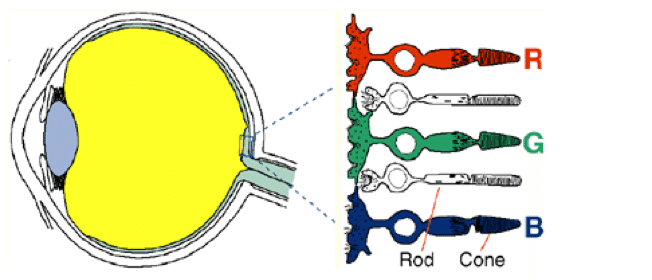
\includegraphics[scale=0.3]{./Images/eyes.jpeg}

{\it \footnotesize Cones of the human eye. From Mafalda (2017)}

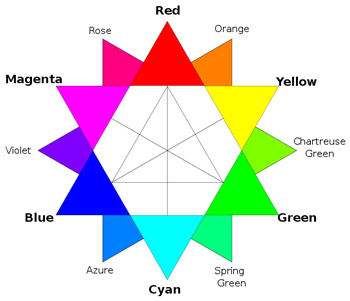
\includegraphics[scale=0.1]{./Images/colorwheel.jpg}

{\it \footnotesize Wheel of colour. From Judge (2012)}
\end{center}

\noindent Firstly, colour is the most straightforward, because it is already commonly divided into primary, secondary and tertiary colours. In psychophysical colorimetry the primary colours red, green and blue are regarded as being \textit{complete}, that is, constituting all human perceptible colours when combined along an axis of light to dark (additive light mixing), yet also being \textit{imaginary}, meaning only existing subjectively as qualia, while not being distinguishable as primaries through ‘objective’ measurement (MacEvoy, 2007). A standard human eye contain three types of light receptor cones, one for each of the three colours. 

All qualia that exist as polarities on a spectrum will be reduced to a semantic prime for the spectrum, combined with the particles for \textit{positive/high, neutral} and \textit{negative/low.} Translating this into an oligosynthetic semantic colour inventory, we would get the following (capitalised letters representing some as of yet undetermined but fixed assigned syllable): 

SHADES: 
\begin{itemize}

\item    Black/dark: JE.LAS \je \las (= negative + brightness) 

    \item White/light: FO.LAS \fo \las (= positive + brightness) 
\end{itemize}
\quad

PRIMARY: 
\begin{itemize}

    \item Red: EL \el 

    \item Green: OS \os 

\item Blue: UL \ul 
\end{itemize}
\quad


SECONDARY AND TERTIARY (RGB is chosen as fixed order): 

\begin{itemize}
\item   Orange: EL.OS \el \os 

\item   Cyan: OS.UL \os \ul 

\item   Magenta: UL.EL \ul \el 

\item   Orange: EL.OS.EL \el \os \el 

\item   Chartreuse green: EL.OS.OS \el \os \os 

\item   Spring green: OS.UL.OS \os \ul \os 

\item   Azure: OS.UL.UL \os \ul \ul 

\item   Violet: UL.EL.UL \ul \el \ul 

\item   Rose: UL.EL.EL \ul \el \el 
\end{itemize}

In 1969, anthropologist Brent Berlin and linguist Paul Kay published their book \textit{‘Basic Color Terms’} in which they proposed their research concerning the prevalence and development of different colour terms in languages from around the world (Berlin \& Kay, 1969). They proposed a chronological scheme of seven evolutionary stadia through which languages generally add colour terms to their lexicon. These are as follows: 

\begin{itemize}
\item Stage I: dark-cool (>‘black’) \& light-warm (>‘white’) 

\item Stage II: red 

\item Stage III:  green OR yellow 

\item Stage IV:  green AND yellow 

\item Stage V:  blue 

\item Stage VI:  brown 

\item Stage VII:  purple, pink, orange or gray 
\end{itemize}

Atlan, needing to conform to constraint 1, cultural neutrality, should thus contain these colours in its lexicon. Stage I-V have already been accounted for, and stage VI and VII can be covered by the combination of the colours from the earlier stages (following the order of shade-XYZ and primary-secondary-tertiary): 

\begin{itemize}
    \item Brown: red + green + blue  = ´EL.OS.UL´ \el \os \ul 

    \item Pink: white + red à = ´FO.LAS.EL´ \fo \las \el 

    \item Gray: colour + brightness + neutral = ´KAL.UJ.LAS´ \kal \uj \las 
\end{itemize}

All other colours and shades can be achieved using this combinatory system. One might argue that not all languages have the same lexical colour inventory, and some make more or less distinctions than English, but it should be noted that having a word for a specific colour is not the same as being able to perceive these different colours and their (subtle) differences (weak linguistic determinism, see chapter 1). Within the line of thought of linguistic determinism, one could argue that learning to speak Atlan, as having this colour system, would gift the speaker with an intuitive understanding of the composition of phenomenal color. 

Besides colour, three-dimensional shape is the other primary irreducible element within vision, constituting what in cognitive science is known as Gestalt (Rollinger \& Ierna, 2019). This term is also applicable to proportional ‘shapes’ or patterns within other qualia, like a musical melody. Visual shape can be geometrically reduced to lines/sides (1D), corners, surfaces (2D), angles and volumes (3D), making use of numerals to specify the quantities of these elements, as well as spatial prepositions to indicate relative location. This, however, will be further expounded upon in chapter 4 of the book, on Atlan’s numerals and mathematics.  


\noindent {\it Sound}

\noindent Sound is commonly divided into three elements:

\begin{itemize}
\item   The frequency of the soundwave, phenomenally corresponding with \textit{pitch}; 

\item   The amplitude of the soundwave, phenomenally corresponding with \textit{volume};

\item   The shape of the soundwave, phenomenally corresponding with \textit{timbre}.

\end{itemize}

%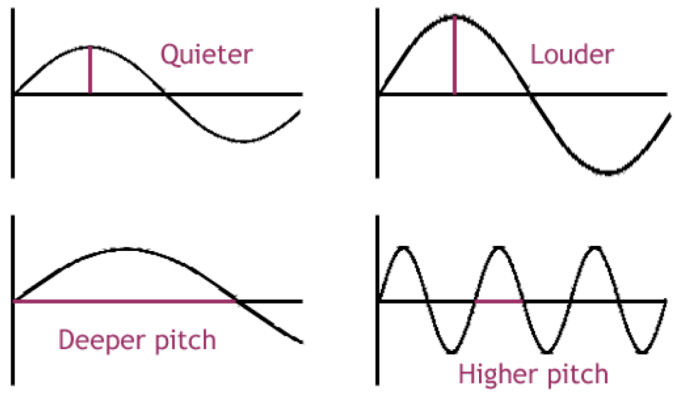
\includegraphics[scale=0.4]{./Images/Frequency.jpeg}

{\it \footnotesize Frequency visualised. From Mata (2015).}

\quad

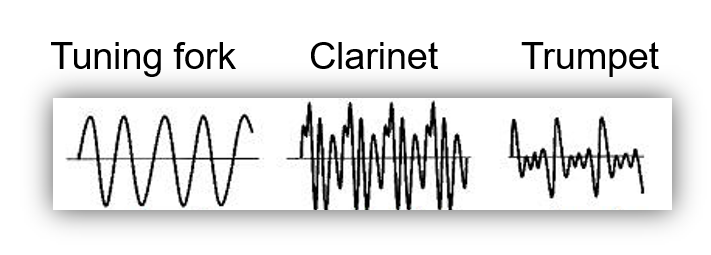
\includegraphics[scale=0.4]{./Images/Timbre.jpeg}

{\it \footnotesize Timbre. From SimplifyingTheory (n.d.).}


Music theory almost universally divides \textbf{pitch} into a \textit{scale}  of notes, which repeats at the ‘octave’, where the ratio to the first note of the previous scale is 2:1. Western music uses the \textit{diatonic} scale, comprised of specifically alternating whole and half steps, and which is \textit{heptatonic} because it is comprised of 7 notes, before repeating at the octave (8th). There are a total of 12 half note steps within an octave, which comprise the \textit{chromatic} scale. Chromatic notes are specified relative to the \textit{natural} (♮) heptatonic scale, by indicating a half step lower by a \textit{flat} (♭) and a half step higher by a \textit{sharp}  (♯). 


\begin{wrapfigure}{r}{0.4\textwidth}
%\includegraphics[scale=0.4]{./Images/pitch.jpeg}
\end{wrapfigure}

The diatonic scale is not the most prevalent musical scale in the world, however, but rather the \textit{pentatonic} scale (five notes) (Encyclop\ae dia Britannica, inc., n.d.). However, a pentatonic scale fits neatly within a heptatonic scale, for example: C–D–E–G–A is a pentatonic scale which only omits the notes F and B. Because of this, Atlan shall use a system based on the Western heptatonic scale, while remaining culturally neutral because this system also accommodates the more common pentatonic scale. If it were to use the pentatonic scale as the standard, the heptatonic scale would be an extended modification, which would be quite clumsy seeing as Western music is so vast and globalised. 

Notes will be indicated with a context-dependent optional semantic prime for \textit{note/pitch} in front of the note name. The combination {\it note} + the first 7 numerals (see chapter 6.2) can be taken to represent the 7 notes (heptatonic: \textit{IP, OP, UP, IK, OK, UK, IM,} pentatonic: \textit{IP, OP, UP, OK, UK}). This will also make calculating musical intervals more intuitive because it will only require simple mental subtraction. 

Sharp will be indicated by \textit{pitch-positive} (also designating \textit{high} in the context of sound frequency) and flat (also indicating \textit{low} in the context of sound frequency) by \textit{pitch-negative.} Double sharps (!musDoubleSharp) and double flats (!musDoubleFlat ) could be created by reduplicating \textit{positive/negative} respectively. Microtonal notes (which fall in between the chromatic notes) could be accounted for as follows: half-sharp (half sharp ) -PN, half-flat (half flat ) -NP, three-quarter-sharp (three quarter sharp ) -PNP, three-quarter-flat (three quarter flat ) -NPN. Major and minor could be designated by the semantic primes for \textit{happy} and \textit{sad} (see the subchapter Emotions), and the seven scale modes could simply be numbered. Harmonic music theory is way too elaborate and complicated to cover fully in this paragraph, however it could be fairly easily constructed from the building blocks presented here. 

Volume is a lot simpler: within music theory it is known as dynamic, and divided into loud (Italian: \textit{forte, f}) and soft (Italian: \textit{piano, p}), further nuanced by the prefix medium (Italian: \textit{mezzo}), and by introducing a three-degree scale of intensity \textit{(ppp, pp, p, mp, mf, f, ff, fff)}. Adopting this system, Atlan can specify volume by combining the semantic prime for \textit{volume} with \textit{positive, medium, negative,} and a \textit{comparative/superlative} system, which will also be applied in other places of the language: \textit{X, more X, most X.} Changes in dynamic (growing louder, \textit{crescendo}, or softer, \textit{decrescendo}) can be described by the semantic primes for \textit{becoming} combined with \textit{more-volume-positive/negative.} 

Finally, timbre, corresponding with the specific shape of the soundwave pattern, has an almost infinite range of possible combinations. This is why in language, terms that denote timbre are always metaphoric approximations, describing the sound with words that denote phenomena unrelated to sound when taken literally, but have a similar phenomenal quality to the sound (e.g., piercing, empty, dark, bright), or are related to the origin of the sound (e.g., nasal, metallic). P. Sesuni analysed 45 studies on different timbre terms in English, Japanese, French, Czech, Swedish, Dutch, Finish, Spanish and German, and from these, identified 59 different descriptors (see appendix 1) (Susini, Carron, Rotureau, Dubois, \& Misdariis, 2017). 

Because these are all semantically reducible to non-sound-related terms, Atlan will not have any timbre-specific semantic primes, but rather use these and other timbre-descriptors, preceded by the semantic prime denoting \textit{sound}, combined with an adjective-marker. When occurring in a clearly sound-related context, the \textit{sound} prime may even be omitted, as there might not be any semantic confusion when it is already obvious that the adjective refers to a sound. 







\chapter{Lexicon -- {\small Jep Antonisse}}
\lettrine{A}{ccording} to research by First Education (2022), the Dutch are positioned as the most proficient English-speaking population globally. Other countries that achieved a position in the top 10 ranking were Denmark, Belgium, Sweden, Finland, and Germany. While a proud Dutchman may attribute this success to hard work and dedication, it is worth considering other factors that could be at play here. Notably, these countries with commendable English proficiency are all located in North Europe and speak very similar languages.  

Linguistics offers a unique perspective on the relationships between different languages. By comparing the vocabulary, grammar\idx{grammar} and sound\idx{sound} systems of various languages, researchers have identified related language families and have constructed language family\idx{language family} trees to illustrate the evolution and divergence of languages over time. Thanks to that research, we know that many countries with notable position in the English Proficiency Index share a common linguistic background . Such a linguistic background , or language family\idx{language family}, thus may provide a foundation for proficiency in a new language. 

This would imply that certain languages are easier to learn for certain population groups. For Atlan, it is deemed important that it will become a language that is easy and quick to learn for \textit{everybody}. This is a challenging task but might be achievable if we find some sort of shared background  between almost every natural language. If it is possible to find words that look similar in different languages, which are known as cognate\idx{cognate}s, the translation\idx{translation} for those words in Atlan can be designed to resemble them as much as possible. With a model that can do this on a large scale, Atlan will become easy, neutral, and global.  

To achieve this, it is first key to create some understandings of what methods are used to compare different languages. Therefore, we will take a closer look at the so-called cosine similarity. Thereafter, it is necessary to conduct an examination of the existing language families that exist. In that way, we gain a deeper insight into the connections between existing natural languages. In addition, with that gained understanding, it is possible to decide which language we will make available in contributing to the process of cognate\idx{cognate} finding. The most spoken languages are weighed against each other to create a dataset that is representative of the real world. All these pieces of the puzzle come together in the final part of this chapter, where the computer program that we used to generate words in Atlan will be discussed.

\section{Comparison methods and language families}

\subsection{Cosine Similarity}

\begin{center}
\resizebox{1\textwidth}{!}{
\begin{tabular}{|c|c|c|}
\hline
{\bf Text} & {\bf Frequency \lq\lq Merry"} & {\bf Frequency \lq\lq christmas"} \\
\hline

\lq\lq Merry christmas " & 1 & 1 \\

\lq\lq Christmas" & 0 & 1 \\
\hline
\end{tabular}
	}

{\it \footnotesize Table 6.1: Word-appearance in \lq\lq Merry" and \lq\lq Merry christmas".}
\end{center}

 \noindent This table can be visualized in a two-dimensional array, where on each axis the count of a word is represented. Now both texts can be placed as a dot on this grid accordingly. Drawing two lines from each point to the origin of the grid creates an angle between those lines. This angle at the origin can be calculated, in this case it would be 45$^{\circ}$ . To finish the cosine similarity, all that is needed now is to take the cosine of this angle, in this example \textit{cos (45)} = 0.71. 


\begin{center}
	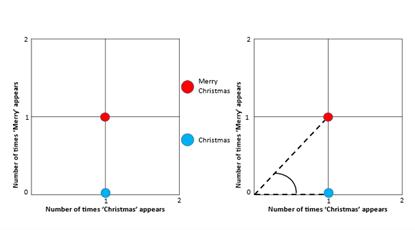
\includegraphics[scale=0.6]{./Images/graphs.jpg}

	{\it \footnotesize Figure 6.1: Graph depicting word-appearance}
\end{center}

If the compared sentences are identical, the two dots would be placed on the same place in the grid. Thus, the lines towards the origin would fall precisely over each other. Therefore, the angle between both lines would be 0$^{\circ}$, resulting in a cosine score of \textit{cos (0) = 1.} On the other hand, if both sentences have not a single element in common, the lines would be perpendicular to each other. With an angle of 90$^{\circ}$, the cosine similarity would return \textit{cos (90) = 0.} Thus, in any case, the cosine similarity gives a score between 0 and 1, showing the degree of similarity. 

As another example, let’s compare two words: \textit{‘Bert’} to \textit{‘Ernie’}. Instead of words, the vector now can be made up of letters. In a table, this would look like this:

\begin{center}
\begin{tabular}{|l|c|c|c|c|c|c|c|}
\hline
{\bf Name} & {\bf E} & {\bf R} & {\bf N} & {\bf I} & {\bf B} & {\bf T} \\
\hline
{\bf Ernie} & 2 & 1 & 1 & 1 & 0 & 0\\
{\bf Bert} & 1 & 1 & 0 & 0  & 1 & 1 \\
\hline
\end{tabular}

{\it \footnotesize Table 6.2: Letter frequency in the words \lq\lq Bert" and \lq\lq Ernie".}
\end{center}

\noindent With six different letters occurring, it would be possible to place both \textit{‘Bert’} and \textit{‘Ernie’} in a six-dimensional grid and draw the lines to the origin. However, it is impossible for humans to visualize a six-dimensional graph. Thus, we need a new way to calculate the angle between the two vectors. Luckily, there exists a formula to compute the cosine similarity. 

\begin{center}
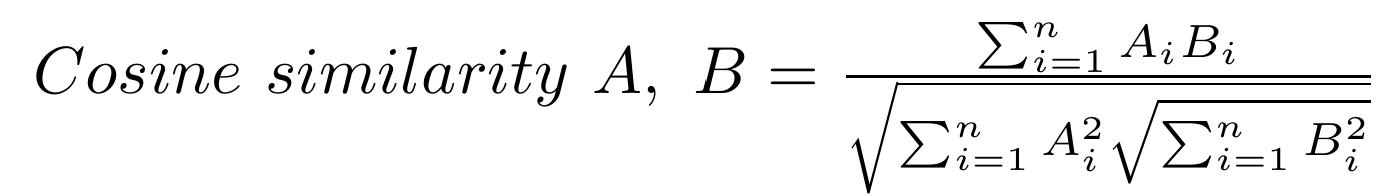
\includegraphics[scale=0.2]{./Images/cosine.jpeg}
\end{center}

%\begin{center}
%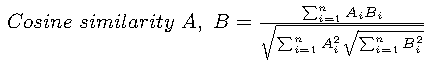
\includepdf[scale=0.5]{./Mainmatter/sum.pdf}
%\end{center}
%\end{samepage}

%\begin{equation}
%Cosine~ similarity~ A, ~B = \frac{\sum_{i=1}^{n} A_i B_i}{\sqrt{\sum_{i=1}^{n} A_i^2 \sqrt{\sum_{i=1}^{n} B_i^2}}}
%\end{equation}

In less mathematical terms, what this means is that each element of the two vectors A and B are compared. The products of all the elements are then summed up and divided by the length of both the vectors together. If we fill in the numbers for our Bert-Ernie-comparison, it will look like this: 

%\resizebox{1\textwidth}{!}{
{\footnotesize
%\begin{equation}
	\[
	\frac{1 \times 2 + 1 \times 1 + 1 \times 0 + 1 \times 0 + 0 \times 1 + 1 \times 0}{\sqrt{2^2 + 1^2 + 1^2 + 1^2 + 0^2 + 0^2 \sqrt{1^2 + 1^2 + 0^2 + 0^2 + 1^2 + 1^2}}} = 0.56
\]
%\end{equation}
%}
}

Nevertheless, converting the words based solely on letter frequency inadvertently results in losing vital information about the arrangement of the letters. This preservation is of utmost importance for our project since we try to find patterns and therefore adjacent letter combinations. To address this concern, we introduced a slight adjustment to the regular cosine similarity, where each index with the same character in both words also scores a small point. In this way, our cosine similarity tries to reward words that have the same letters on the same place.

\subsection{Language families}

The use of various comparison methods, similar to the cosine similarity, allowed linguists to identify groups of related languages. These groups, or language families, were categorized based on common linguistic features and a shared common ancestor (Campbell, 2018). Such a common Proto-Language allows researchers to trace origins of various languages to a single root. However, this does not necessarily need to be the case. There exist languages for which it is impossible to classify them as part of a language family\idx{language family}, such as Basque (Campbell, 2010). Researchers speculate that it might be possible that these languages, known as language isolates, might have had related languages in the past, that went extinct unrecorded. Therefore, these languages now form their own language family\idx{language family}, with them being the only member. On the other hand, not only genetic proximity between languages is enough to be placed in the same language family\idx{language family}. Languages that are constructed instead of naturally developed cannot be considered part of any language family\idx{language family}, since they do not have a shared ancestor with any other language (Campbell, 2018). 

Although this means that the total number of language families in the world might be in the hundreds, not all are equally relevant today. To begin with, 94 language families are extinct, meaning there is a lack of any surviving speakers (Campbell, 2018). In addition, the number of languages and the number of speakers differ largely. There are five language families that can be considered as the main language families of the world. Every single one of these languages contains at least 5\% of the languages in the world and combined they capture more than two-thirds of all the natural languages. The families are called Indo-European, Sino-Tibetan, Niger-Congo, Austronesian and Afro-Asiatic.  

\hyphenation{Ukrain-ian}
The most widely spoken language family\idx{language family}, with over 3 billion speakers worldwide today, is Indo-European. When Sir William Jones first spoke of this family, he proposed there were several branches with related languages (Fortson, 2011). First, there is \textit{Indo-Iranian}, spoken in the middle east, where the languages Sanskrit, Persian and Pashto are placed. Secondly, \textit{Italic}, with languages such as Latin, Italian and Spanish. Third, the languages of the Northern parts of Europe were placed in the \textit{Germanic} branch. A fourth branch called \textit{Celtic} housed the languages of the island of Great Britain, such as Irish and Welsh. Lastly, Jones portrayed one branch on its own for \textit{Greek}.. Only after thirty years would this division be altered, when researchers added three more branches to the family. The largest new branch was called the \textit{Balto-Slavic} branch, including languages such as Russian, Ukrainian, and Czech. The two remaining branches both only contained one language, \textit{Armenian} and \textit{Albanian.} This family tree remained the same to this day, except for the addition of two branches with extinct languages discovered in the first half of the 20th century, called \textit{Anatolian} and \textit{Tocharian.}  

The Sino-Tibetan language family\idx{language family} is, even though it has more daughter languages than Indo-European, the second most spoken family, with around  1.3 billion speakers. This family can be split up into two major subgroups: \textit{Chinese} and \textit{Tibeto-Burman}  (Shafer, 1955). The Chinese subgroup is like a family on its own, made up of different but related dialects. The largest and best-known ones are Mandarin and Cantone\idx{tone}se. Tibeto-Burman can be branched into three further branches: Tibetic (Tibetan), Burmese-Lolo (Burmese and various Lolo languages) and Karenic.  

Niger-Congo is the third most spoken family, containing the highest number of languages: over 1,500 languages are known ancestors of the Proto-Niger-Congo language. Although this number is nearly twice that of Indo-European, it is spoken by 600 million people, due to the immense language diversity in the Sub-Saharan Africa region (Heine et al., 2000). The largest branch in the Niger-Congo family is called the \textit{Atlantic-Congo} branch. Herein are numerous languages spoken in West Africa, such as Yoruba and Igbo. Also, Swahili, mostly spoken in the Easte\idx{taste}rn part of Africa, falls into this category. The languages spoken in the Central and Southern parts of Africa are mostly from another branch, called the \textit{Bantu-Congo} branch. These are languages such as Zulu, Xhosa and Shona. Other branches are the \textit{Kordofanian} branch (Katla, Moro and Talodi) and \textit{Mande} branch (Bambara, Mandinka and Soninke) 

Austronesian, with a similar high diversity as Niger-Congo, covers the languages found  in the region that stretches from Southeast-Asia to the Pacific Island. In total this family contains more than 1,200 languages and is spoken by approximately 326 million speakers, mostly in countries such as Indonesia, Malaysia and the Philippines. The most important subgroup within this family is the \textit{Formosan} branch, forming a total of nine distinct branches (Tryon, 1995). These branches are all made up of the different indigenous languages of Taiwan. None of them are, however, the most widespread or diverse branch of the family. This is namely the tenth branch, known as the \textit{Malayo-Polynesian} branch, encompassing Indonesian, Javanese and Sundanese.  

Lastly, the languages mostly spoken in the North and the Horn of Africa and Southwest Asia are grouped in the Afroasiatic language family\idx{language family}.  This family consists of several branches (Huernergard, 2004). The branch that houses the best-known languages is the \textit{Semitic} branch, including Arabic, Amharic\idx{Amharic} and Hebrew. Another large branch is \textit{Berber}, with languages such as Tamazight and Kabyle. Smaller branches are the \textit{Cushitic} branch, which comprises of languages such as Oromo, Somali and Afar, and the \textit{Chadic} branch, with as largest language Hausa. The languages in the Afroasiatic family combined are spoken worldwide by almost 600 million people. 


\section{Using cognate\idx{cognate}s to generate words}


A study by Otwinowska and Szewczyk (2018) argued that cognate\idx{cognate}s, similar sound\idx{sound}ing words with the same meaning in different languages, are the easiest words to learn when learning a new language. The resemblance with your mother tongue makes the words much easier to remember and use then non-cognate\idx{cognate}s words. By designing Atlan in a way that it has a lot of these cognate\idx{cognate}s, we try to keep the trouble of learning Atlan as low as possible. To achieve this goal, it is key to make new Atlan words resemble existing words, or patterns in existing words, as much as possible. 

The idea of using cognate\idx{cognate}s to generate new words for vocabulary is also used in the creation of the constructed language Lojban\idx{Lojban} (Cowan, 1997).  Lojban\idx{Lojban} proposed new words, or ‘gismu’s’ and looked for words that looked similar to it in the languages Chinese, English, Spanish, Hindi, Russian and Arabic. If three or more letters were the same and in the same order as a word in the source language, the gismu would score points. For resemblance with larger language a gismu could score more points, meaning that large languages were viewed as more important. The amount of influence each language had, in other terms the ‘weight’, was solely based on the number of speakers in 1985.  

For Atlan we have built a similar program, which we will call \textit{Lexi\idx{Lexi}} from now on. To understand how Lexi\idx{Lexi} works, it is wise to split the process into three parts: the language selection, the weights, and the program itself.  

\subsection{Language selection }

The choice made by the developers of Lojban\idx{Lojban} to use the six largest languages was good in terms of significance. Their language set closely resembles the set of UN languages: Chinese, English, Spanish, French, Russian and Arabic. For 49.6\% of all people, these languages are either their mother tongue or second language and form an official language for more than half the states in the world, according to Ethnologue. However, the developers failed to take language families into account. This results in the facts that four out of the six languages used, or two thirds, are a descendent of Proto-Indo-European, while other large families such as Niger-Congo or Austronesian are not represented at all. Distributions so far away from the real world might make the result very Eurocentric. This creates a large group of language learners unable to match any words to their native language. For Atlan to improve on this, the number of languages that is used as a source must be increased. 

Also, if the desired distribution should resemble the distribution of the real world, we need to know what the distributions in the real world \textit{are}. The frequency of each language family\idx{language family} in the 100 most spoken languages according to Ethnologue (2022) can provide a target percentage of how big the part of each language family\idx{language family} should be in our program.  

Now we will create a \textit{language set} or \textit{data set}, with in it all the languages we want to find cognate\idx{cognate}s in. It is important that the cognate\idx{cognate} and the Atlan word has the same meaning in all these languages: otherwise, it might find similar looking words, but with different meanings in different languages, which are known as \textit{false cognate\idx{cognate}s}. These cognate\idx{cognate}s are not a sign of a common ancestor but rather a display of randomness and luck. Also, these false cognate\idx{cognate}s are the most difficult words to learn in a new language, even more difficult than non-cognate\idx{cognate} words (Otwinowska et al., 2018). Hence, we should avoid creating those in Atlan. To do so, we must be able to control the meaning of the words in other languages. 

Translation\idx{translation} software can get us this control. We will use the public available library called Googletrans (3.0.0). This software supports translation\idx{translation} into 107 different languages. Since we desire the same significance the language set of Lojban\idx{Lojban} had, we can analyze which of these languages are present in the list of the 100 most spoken languages. The result can be viewed in these tables: 

\newcounter{tablecount}
\setcounter{tablecount}{1}
\begin{center}
\resizebox{1\textwidth}{!}{
\begin{tabular}{|c|c|c|c|c|}
	\hline
	{\bf Number} & 
	{\bf Language } &
	

	\thead{\bf Number of Native \\ 
	\bf speakers in Millions } &
	

	\thead{\bf Number of Total \\ \bf speakers in Millions } &
	

	\thead{\bf Language family\idx{language family} \\  \bf of the language} \\

	\thetablecount\stepcounter{tablecount}& 
English &
	

379 &
	

1132 &
	

Indo-European \\

	\thetablecount\stepcounter{tablecount} &

Mandarin Chinese &
	

918 &
	

1117 &
	

Sino-Tibetan \\

	\thetablecount\stepcounter{tablecount} &
Hindi &
	

341 &
	

615 &
	

Indo-European \\

	\thetablecount\stepcounter{tablecount} &
Spanish &
	

460 &
	

534 &
	

Indo-European \\
	\thetablecount\stepcounter{tablecount} &

French &
	

77 &
	

280 &
	

Indo-European \\

	\thetablecount\stepcounter{tablecount} &
Standard Arabic &
	

108 &
	

274 &
	

Afro-Asiatic \\

	\thetablecount\stepcounter{tablecount} &
Bengali &
	

228 &
	

265 &
	

Indo-European \\

	\thetablecount\stepcounter{tablecount} &
Russian &
	

154 &
	

258 &
	

Indo-European \\

	\thetablecount\stepcounter{tablecount} &
Portuguese &
	

221 &
	

234 &
	

Indo-European \\
	\thetablecount\stepcounter{tablecount} &

Indonesian &
	

43 &
	

119 &
	

Austronesian \\

	\thetablecount\stepcounter{tablecount} &
Urdu &
	

69 &
	

170 &
	

Austronesian \\
	\thetablecount\stepcounter{tablecount} &

Standard German &
	

76 &
	

132 &
	

Indo-European \\
	\thetablecount\stepcounter{tablecount} &

Japanese &
	

128 &
	

128 &
	

Japanic \\

	\thetablecount\stepcounter{tablecount} &
Swahili &
	

16 &
	

98 &
	

Niger-Congo \\
	\thetablecount\stepcounter{tablecount} &

Marathi &
	

83 &
	

95 &
	

Indo-European \\

	\thetablecount\stepcounter{tablecount} &
Telegu &
	

82 &
	

93 &
	

Dravidian \\
	\thetablecount\stepcounter{tablecount} &

Western Punjabi &
	

93 &
	

93 &
	

Indo-European \\

	\thetablecount\stepcounter{tablecount} &
Tamil &
	

75 &
	

81 &
	

Dravidian \\

	\thetablecount\stepcounter{tablecount} &
Turkish &
	

69 &
	

80 &
	

Turkic \\

	\thetablecount\stepcounter{tablecount} &
Korean\idx{Korean} &
	

77 &
	

77 &
	

Korean\idx{Korean}ic \\

	\thetablecount\stepcounter{tablecount} &
Vietnamese &
	

76 &
	

77 &
	

Sino-Tibetan \\

	\thetablecount\stepcounter{tablecount} &
Javanese &
	

68 &
	

68 &
	

Austronesian \\

	\thetablecount\stepcounter{tablecount} &
Italian &
	

65 &
	

68 &
	

Indo-European \\
	\thetablecount\stepcounter{tablecount} &

Hausa &
	

44 &
	

63 &
	

Afro-Asiatic \\

	\thetablecount\stepcounter{tablecount} &
Thai &
	

21 &
	

61 &
	

Kra-Dai \\
	\thetablecount\stepcounter{tablecount} &

Kannada &
	

44 &
	

56 &
	

Dravidian \\

	\thetablecount\stepcounter{tablecount} &
Filipino &
	

0.125 &
	

45 &
	

Austronesian \\

	\thetablecount\stepcounter{tablecount} &
Polish &
	

40 &
	

40 &
	

Indo-European \\
	\thetablecount\stepcounter{tablecount} &

Yoruba &
	

38 &
	

40 &
	

Niger-Congo \\
	\thetablecount\stepcounter{tablecount} &

Odia &
	

34 &
	

38 &
	

Indo-European \\

	\thetablecount\stepcounter{tablecount} &
Malayalam &
	

37 &
	

38 &
	

Dravidian \\
	\thetablecount\stepcounter{tablecount} &

Ukrainian &
	

27 &
	

33 &
	

Indo-European \\
	\thetablecount\stepcounter{tablecount} &

Sudanese &
	

32 &
	

32 &
	

Afro-Asiatic \\
	\thetablecount\stepcounter{tablecount} &

Zulu &
	

12 &
	

28 &
	

Niger-Congo \\
	\thetablecount\stepcounter{tablecount} &

Igbo &
	

27 &
	

27 &
	

Niger-Congo \\
	\thetablecount\stepcounter{tablecount} &

Amharic\idx{Amharic} &
	

22 &
	

26 &
	

Afro-Asiatic \\
	\thetablecount\stepcounter{tablecount} &

Uzbek &
	

25 &
	

25 &
	

Turkic \\
	\thetablecount\stepcounter{tablecount} &

Nepali &
	

16 &
	

25 &
	

Indo-European \\
\hline
\end{tabular}
}
\end{center}

\begin{center}
\resizebox{1\textwidth}{!}{
\begin{tabular}{|c|c|c|c|c|}
\hline
	{\bf Number} & 
	{\bf Language } &
	

	\thead{\bf Number of Native \\ 
	\bf speakers in Millions } &
	

	\thead{\bf Number of Total \\ \bf speakers in Millions } &

	\thead{\bf Language family\idx{language family} \\  \bf of the language} \\
	
\thetablecount\stepcounter{tablecount} &

Sindhi &
	

25 &
	

25 &
	

Indo-European \\
	\thetablecount\stepcounter{tablecount} &

Romanian &
	

24 &
	

24 &
	

Indo-European \\
	\thetablecount\stepcounter{tablecount} &

Dutch &
	

23 &
	

23 &
	

Indo-European \\

	\thetablecount\stepcounter{tablecount} &
Pashto &
	

21 &
	

21 &
	

Indo-European \\

	\thetablecount\stepcounter{tablecount} &
Xhosa &
	

8 &
	

19 &
	

Niger-Congo \\

	\thetablecount\stepcounter{tablecount} &
Malay &
	

16 &
	

19 &
	

Austronesian \\
	\thetablecount\stepcounter{tablecount} &

Khmer &
	

17 &
	

18 &
	

Austronesian \\
	\thetablecount\stepcounter{tablecount} &

Afrikaans &
	

7 &
	

18 &
	

Indo-European \\
	\thetablecount\stepcounter{tablecount} &

Sinhala &
	

15 &
	

17 &
	

Indo-European \\
	\thetablecount\stepcounter{tablecount} &

Somali &
	

16 &
	

16 &
	

Afro-Asiatic \\

	\thetablecount\stepcounter{tablecount} &
Cebuano &
	

16 &
	

16 &
	

Austronesian \\
	\thetablecount\stepcounter{tablecount} &

Kurdish &
	

15 &
	

15 &
	

Indo-European \\

	\thetablecount\stepcounter{tablecount} &
Azerbaijani &
	

14 &
	

14 &
	

Turkic \\

	\thetablecount\stepcounter{tablecount} &
Czech &
	

11 &
	

13 &
	

Indo-European \\
	\thetablecount\stepcounter{tablecount} &

Greek &
	

13 &
	

13 &
	

Indo-European \\
	\thetablecount\stepcounter{tablecount} &

Kazakh &
	

13 &
	

13 &
	

Turkic \\
	\thetablecount\stepcounter{tablecount} &

Swedish &
	

10 &
	

13 &
	

Indo-European \\
	\thetablecount\stepcounter{tablecount}& 

Hungarian &
	

13 &
	

13 &
	

Uralic \\
\hline

\end{tabular}
}
\end{center}

\vspace{0.1cm}
{\it \footnotesize Table 6.3: Overview of the languages and their number of speakers according to Ethnologue (2022).}
\vspace{0.3cm}


\noindent Assume that this entire set of 57 possible languages becomes the dataset, called set \alpha. Then it is possible to find the frequencies of each family in the \alpha set. Since we want to compare these numbers relative to the total amount of languages, we need to convert these frequencies to percentages by dividing them by the total number of languages in set \alpha, which is 57. Now it is possible to compute the distance between the current percentage and the target percentage by taking the absolute of the target number minus the current percentage. This is called the error rate. So, for Indo-European, the error rate would be |42 – 43.9| = |-1.9| = 1.9, meaning that is almost 2\% away from the target percentage. We can do this calculation for every language family\idx{language family}, and the result can be viewed in the fourth column of table 6.5. The error values average to an average error rate of 2.76. Meaning that on average each language family\idx{language family} is either 1.58 languages too large or too little. This is not a bad score, but it is possible to make this error figure smaller by adding and removing some languages to counterbalance. 

The Indo-European language family\idx{language family} is very well represented, with almost a language from each branch or otherwise a very similar language present. Thus, we leave those 25 languages untouched. We want those 25 languages to make up for 42 percent of the set, thus we need 100\% of the dataset to be around  (24/42 $\times$ 100) $\approx$ 60 languages. With the current 57, we should be able to add three more languages. 

However, there is one language family\idx{language family} that is far too overrepresented. Almost all the languages in the top 100 from the Austronesian family made it into the  database, while they should be less frequent than Afro-asiatic and Niger-Congo. Therefore, we remove one language from this language family\idx{language family}: Malay. Even though there are several less spoken Austronesian languages, the older common ancestor between these languages (Tryon, 1995) entails that these may contain more vital information about a group of languages not seen in the data. The only exception is Filipino, which is a language that is derived from the already present in the $\alpha$-language Tagalog, meaning they are also very similar. The choice to let Filipino stay is due to the interesting fact that it has much more speakers than a lot of languages, even though it has a relative low number of native speakers. This aspect of the language might be a good contribution to the desired ‘easy-to-learn-aspect.’ This reduces the number of present languages to 56, so we can add four new languages. 

The language-family with the largest error is Sino-Tibetan. There is only one language that could be seen as Sino-Tibetan, although not all linguists would agree. Hmong is classified as part of the Hmong-Mien languages. Most Chinese scholars have accepted that it is part of Sino-Tibetan family (Matisoff, 1991). Although linguists outside of Europe have a narrower view of Sino-Tibetan, they at least agree that the Hmong-Mien languages are strongly influenced by Chinese languages. Therefore, we will add Hmong to the data set and count is as a Sino-Tibetan language. Even with Hmong added the Sino-Tibetan family seems underrepresented. However, we need to keep in mind that a lot of the languages in the top 100 most spoken languages are a form of Chinese and strongly related to Mandarin, which is present in the data set. 

Now three languages remain to be added for the other underrepresented languages: Niger-Congo and Afroasiatic. Afroasiatic has a higher frequency in the 100 most spoken languages, but they are currently both equally present. This means we should give Afro-asiatic two extra languages and Niger-Congo only one.  

For Afroasiatic we can translate into Hebrew and Maltese, both Semitic languages. Thus, we don’t need to make any choices here. In the Niger-Congo family we can choose between Shona, Sesotho and Chichewa. Since they are all the same branch, we choose the one with the most speakers, which is Chichewa.   

\begin{center}
\resizebox{1\textwidth}{!}{
\begin{tabular}{|c|c|c|c|}
	\hline
	{\bf Language } &
	

	\thead{\bf Number of Native \\ 
	\bf speakers in Millions } &
	

	\thead{\bf Number of Total \\ \bf speakers in Millions } &
	

	\thead{\bf Language family\idx{language family} \\  \bf of the language} \\
	\hline

	Hmong &
	

	8 &
	

	8 &
	

	Sino-Tibetan \\ 

	Hebrew &
	

	7 &
	

	9 &
	

Afro-asiatic \\

	Maltese &
	

	0.5 &
	

	0.5 &
	

Afro-asiatic \\

	Chichewa &
	

	9 &
	

	9 &
	

Niger-Congo \\ 
\hline
\end{tabular}
}

\vspace{0.1cm}
{\it \footnotesize Table 6.4: Information about the new languages chosen for the dataset.}
\end{center}

\noindent With this modification to set $\alpha$, we have a new set of languages, we can call language set . By calculating the errors again for each language family\idx{language family}, we can see that the error measure now averages to an amazing 1.83. Meaning that on average a family is 1.1 language off from the real distribution. These are distributions that are very realistic to the real world. 

\vspace{-0.1cm}
\begin{center}
%	\begin{adjustbox}{angle=90}
\resizebox{1\textwidth}{!}{
	\large
\begin{tabular}{|c|c|c|c|c|c|c|c|}
	\hline
	{\bf Language family\idx{language family}} &
	

\thead{\bf \footnotesize Frequency in the \\ \bf 100 most spoken \\ \bf languages}& 
	

\thead{\bf \footnotesize Frequency in the \\ \bf $\alpha$ set} & 
	

\thead{ \bf \footnotesize Percentage in the \\ \bf $\alpha$ set }& 
	

\thead{\bf \footnotesize Error in the \\ \bf $\alpha$ set} & 
	

\thead{\bf \footnotesize Frequency in the \\ \bf $\beta$ set} & 
	

\thead{\bf \footnotesize Percentage in the \\ \bf $\beta$ set}& 
	

\thead{\bf \footnotesize Error in the \\ \bf  $\beta$ set}\\ 
\hline

Indo-European & 
	

42 & 
	

25& 
	

43.9& 
	

1.9& 
	

25& 
	

41.6& 
	

0.4\\ 

	Afro-Asiatic &
	

15& 
	

5& 
	

8.8& 
	

6.2& 
	

7& 
	

11.6& 
	

3.4\\ 

Niger-Congo &
	

12& 
	

5& 
	

8.8& 
	

3.2& 
	

6& 
	

10.0& 
	

2.0\\ 

Austronesian &
	

9& 
	

8& 
	

14.0& 
	

5& 
	

7& 
	

11.6& 
	

2.6\\ 

Sino-Tibetan &
	

9& 
	

2& 
	

3.5& 
	

5.5& 
	

3& 
	

5.0& 
	

4\\ 

Turkic &
	

4& 
	

4& 
	

7.0& 
	

3& 
	

4& 
	

6.7& 
	

2.7\\ 

Dravidian &
	

4& 
	

4& 
	

7.0& 
	

3& 
	

4& 
	

6.7& 
	

2.7\\ 

Japanic &
	

1& 
	

1& 
	

1.8& 
	

0.8& 
	

1& 
	

1.7& 
	

0.7\\ 

Uralic &
	

1& 
	

1& 
	

1.8& 
	

0.8& 
	

1& 
	

1.7& 
	

0.7\\ 

Korean\idx{Korean}ic & 
	

1& 
	

1& 
	

1.8& 
	

0.8& 
	

1& 
	

1.7& 
	

0.7\\ 

Kra-Dai &
	

2& 
	

1& 
	

1.8& 
	

0.2& 
	

1& 
	

1.7& 
	

0.3\\ 
\hline
\end{tabular}
}
%\end{adjustbox}
\vspace{0.1cm}

{\it \footnotesize Table 6.5: Frequencies of languages families in different language sets}
\end{center}

\noindent To visually represent the diversity within this set, we provide you with the following map. Each non-blue country in the figure is associated with at least one official or national language present in the dataset. The handful of blue countries indicate the absence of certain languages.  

\begin{center}
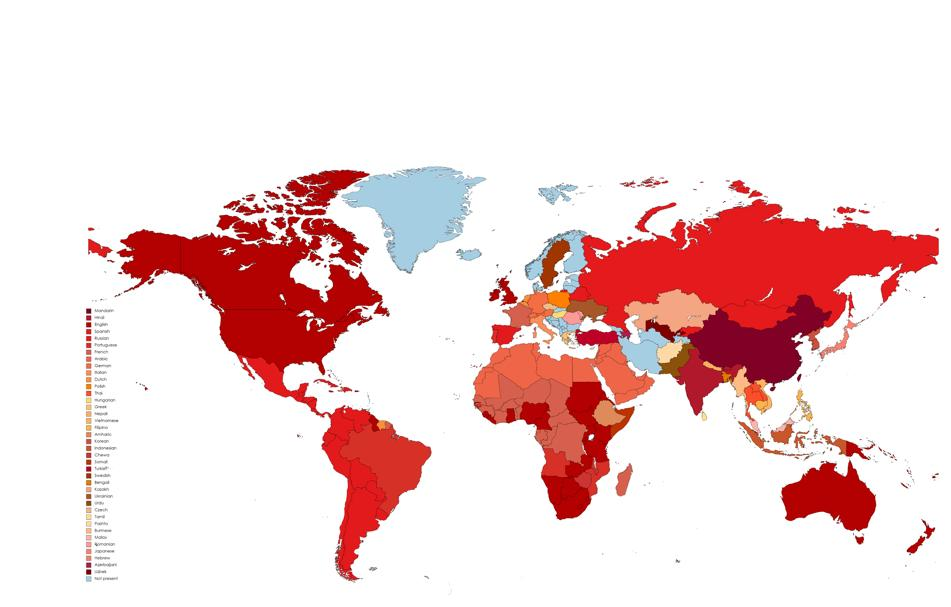
\includegraphics[scale=0.4]{./Images/worldatlas.jpg}

	{\it \footnotesize Figure 6.2: World map to visualize where languages present in the dataset are spoken according to Ethnologue (2022) and WALS (2013), made with mapchart.net} 
\end{center}

\vspace{0.3cm}

\noindent

A closer examination of the blue regions reveals that the Scandinavian, Balkan and Baltic countries predominantly fall into this category. However, it is important to notice that although the language self is not in the dataset, there might be one that is very closely related to it. The languages spoken in Denmark, Norway, Sweden, Finland and Iceland share such close relationships. In cross-border communication, individuals from these regions often just continue using their respective languages (Gooskens, 2007). In the same way, languages in the Balkan region, such as Bosnian and Albanian, share a relatively recent common ancestor with Romanian (Kushniarevich, 2015). This means they still share a lot of vocabulary and grammar\idx{grammar}. Similarly, the Baltic states exhibit, although there are fewer resemblances, notable similarities with languages such as Hungarian. Hence, these languages are not entirely absent of the data set.

We can do the same observation for the blue countries outside of Europe. Persian, as the official language of Iran, displays strong connections with Kurdish and Pashto and in lesser terms also with Hindi and Bengali (Fortson, 2011). Additionally, due to the high trade during the Mongol empire, Persian has been largely influenced by Arabic and Turkic languages (Perry, 2005). 

Consequently, the only countries in the world that lack any indication of a Proto-Language connection between their national language and our dataset are Greenland and Armenia. Greenlandic, being an Inuit-language, and Armenian, being a language isolate, show too little similarities with other languages. However, the population of these countries would be less than 4 million people, which accounts for less than 0.05% of the global population of 8 billion people. 

\subsection{Weights}

As discussed previously, the source languages of Lojban\idx{Lojban} with more native speakers were deemed more important (Cowan, 1997). Consequently, the scoring system slightly favoured languages with higher weights, which seems justifiable as it benefits a larger number of individuals. However, the approach employed by Lojban\idx{Lojban} only focused on the number of native speakers of the given language: Chinese had a larger weight then English. The existence of secondary speakers was completely disregarded. 

The -obvious- difference between a native and a secondary speaker is the fact that a native speaker of the language learns while growing up. On the other hand, a secondary speaker acquires a language later in life, motivated by factors such as work, tourism or recreation. By exclusively utilizing native speakers as a metric for assessing the importance of a language, the developers of Lojban\idx{Lojban} missed the crucial information that the secondary speakers provide. The number of secondary speakers conveys a significant insight into both the language's political influence as its reach. (Saville-Troike, 2017). Besides, it can indicate a lot about vitality and the preservation of the language (Grenoble et al, 2005). Moreover, the secondary speaker count offers us more about the ease of learning the language. All of these are factors that are vital for the language Atlan will be. 

As a result, we contend that secondary speakers should not be forgotten and should even be given relatively more weight than native speakers. As a result, the number of total speakers is calculated by 0.4 times the native speakers and 0.6 times the secondary speakers. Subsequently, these adjusted totals are then normalized to obtain the final weights. This way, the largest language contributes the most to the product. 

\subsection{Lexi\idx{Lexi} and her workings}

\noindent With consensus on the dataset and the weights, the time has come to explain how Lexi\idx{Lexi} generates words from all these languages. Lexi\idx{Lexi} is designed to take an English word as input to start the process. This is very important, because there is only a very select group of unreducible words that need to be generated this way. By taking a meaning as input, we prevent that it generates words we do not want and control the meaning of the new Atlan word. 

This word is then translated into all the languages that make up the trainings set that was just discussed. That way we can find a common pattern in this set of 60 translation\idx{translation}s. However, it is key to keep in mind that the same letters are often pronounced differently in different words. For example, the sentence ‘the \textit{tear} in my new painting brought a \textit{tear} in my eye’ contains two words that look identical but sound\idx{sound} very different. Such heteronyms prove it is not enough to compare words only by their spelling. To investigate how words are pronounced, Lexi\idx{Lexi} now transforms every translation\idx{translation} into their IPA\idx{International Phonetic Alphabet} format. 

After the constraints of comparison were a bit hardened by this modification, it is possible to soften them now again. That is, because Atlan reduces the number of vowels\idx{vowels} drastically. This has as a result that certain sound\idx{sound}s that are viewed differently in our languages, can only refer to one and the same letter in Atlan. That means that this sound\idx{sound} can be viewed as the same in comparison. To achieve this, Lexi\idx{Lexi} can map each IPA{International Phonetic Alphabet\idx{International Phonetic Alphabet}} sound\idx{sound} to the letter it would represent in Atlan, according to the rules discussed in the phonology\idx{phonology}-chapter. This creates a list with the transcriptions of how the translation\idx{translation}s would sound\idx{sound} in Atlan.  

\hyphenation{con-sonant-vowel}
The only task that is left now is to find the patterns in this set. Since these patterns will form the new Atlan word, it is certain they will always follow one of three patterns: either con-sonant-vowel-consonant (CVC), con-sonant-vowel (CV) or vowel-consonant (VC). We can look at possible candidates for this pattern by splitting each translation\idx{translation} up into every possible combination that follows one of these patterns. This way, Lexi\idx{Lexi} provides a dataset of candidates of the patterns, made up from small parts of natural language translation\idx{translation}s. 

If we calculate the similarity between every possible pattern and the transcribed translation\idx{translation}s, we can get the pattern that resembles the words best. However, to simulate the natural way of words generation a bit better, we experiment with some algorithms to make sure we pick the best word, such as evolutionary computing. 

This is a problem-solving technique that uses the principles of natural selection and genetics to find patterns and optimal solutions. Just as in nature, the individual with the highest ‘fitness’ are selected to create new children. Generation after generation this will mean that only the best traits survive, resulting in a solution. By using evolutionary computing, we are trying to simulate a natural way of one word evolving over time, with only the fittest words surviving. In this case, a ‘fit’ individual is on average very similar to all the translation\idx{translation}s. We calculate the fitness with the previously discussed cosine similarity. 

The fittest individuals create children through a cross-over process. Lexi\idx{Lexi} divides both words in all possible points and then swaps both halves.  For example, if the words \textit{jap} and \textit{tek} are combined, it can recombine into \textit{j-ek} and \textit{t-ap} and similarly \textit{jak} and \textit{tep.} These children, combined with the parents, form again a large pool of possible Atlan words. The best individuals are again selected, and the winners produce the next generation. After 50 generations, the three individuals with the highest scores are selected and crowned as winners. In the end this process gave us the same outcomes as calculating the highest score for all of them. 

In this way, we generated the five best options for every atom of language we needed to exist in Atlan. Another computer program assigned each word one of these options, keeping in mind that some syllable\idx{syllable}s might appear in the list of options for several words. In the end, this leaves us with a lexicon of words that should be easy to learn and remember for almost the entire population.
\vfill 
\section{Semantic atom\idx{semantic atom} vocabulary}
\vspace{-0.5cm}

\footnotesize
\begingroup
\renewcommand{\numberraise}{-0.15em}
\newcounter{lexi}
\setcounter{lexi}{1}
\newcolumntype{x}[1]{>{\centering\let\newline\\\arraybackslash\hspace{0pt}}p{#1}}
\def\tabb#1{\thelexi.\stepcounter{lexi} #1}
%\hline\end{tabular}%
%\begin{tabular}{|p{0.7\textwidth} | cx{0.2\textwidth}|cx{0.1\textwidth}|}%
%\hline%
\footnotesize
\renewcommand{\corpsgrootte}{12pt}

%	% \begin{tabular}{|l|c|c|}
%	\hline
%	\multicolumn{3}{|c|}{}\\
%	\hline
%		\thelexi.\stepcounter{lexi} & & \\	
%	\hline
%	%\end{tabular}
%}
\begin{center} 
\resizebox{1\textwidth}{!}{%

	%\resizebox{1\textwidth}{!}{
	 \begin{tabular}{|p{0.7\textwidth} | cx{0.2\textwidth}|cx{0.1\textwidth}|}
	%% \begin{tabular}{|l|c|c|}
	\hline
		\multicolumn{3}{|c|}{{\bf MORPHOSYNTAX (V,CV,VC)}}\\
		\hline
		\multicolumn{3}{|c|}{{\bf MOOD MARKERS}}\\ 
	\hline
		\thelexi.\stepcounter{lexi} Exclamative/ 
		imperative/ \newline vocative 
		expletive & O & \Atlano \\	
		\thelexi.\stepcounter{lexi} Interrogative & E & \Atlane \\	
		\thelexi.\stepcounter{lexi} Subjunctive & U & \Atlanu \\	
		\thelexi.\stepcounter{lexi} Stress (prosodic) & A & \Atlana\\	
		\thelexi.\stepcounter{lexi} Relative clause (+ pronoun)& I \newline & \Atlani \\	
	\hline
	%\end{tabular}

	 


%\footnotesize
 
%\resizebox{1\textwidth}{!}{
	% \begin{tabular}{|p{0.6\textwidth} | cx{0.2\textwidth}|cx{0.2\textwidth}|}
	\hline
	\multicolumn{3}{|c|}{\bf LOGICAL OPERATORS}\\
	\hline
		\thelexi.\stepcounter{lexi} Conjunction (and, $\wedge$) & AN & \an \\	
		\thelexi.\stepcounter{lexi} Disjunction (or, $\vee$) & OL & \ol \\	
		\thelexi.\stepcounter{lexi} Conditional (if, $\rightarrow$, {\it ceteris paribus)} & IF & \Atlanif \\	
		\thelexi.\stepcounter{lexi} Conclusion (thus,  therefore $\therefore$) & IS & \is \\	
		\thelexi.\stepcounter{lexi} Negation (not, $\neg $) - sentential/predicate & NE & \Atlanne \\	
		\thelexi.\stepcounter{lexi} All ($\forall$, universal) & AT & \at \\
		\thelexi.\stepcounter{lexi}Some ($\exists$, -few +many) & SO & \so 	\\
		\thelexi.\stepcounter{lexi} Possible ($\diamond$) & PE & \pe \\	
		\thelexi.\stepcounter{lexi} Necessary ($\square$) & SE & \se \\	
	\hline
	%\end{tabular}
	
 


%%\resizebox{1\textwidth}{!}{ \footnotesize
	%% \begin{tabular}{|l|c|c|}
 
	% \begin{tabular}{|p{0.6\textwidth} | cx{0.2\textwidth} | cx{0.2\textwidth}|}
	\hline
		\multicolumn{3}{|c|}{{\bf SYNTACTICAL MARKERS}}\\
	\hline
	\thelexi.\stepcounter{lexi} Accusative (affected thing/person, object, + verb = transitive  & EK & \ek \\	
		\tabb{Genitive (possession,  + verb = to have)} & TA & \ta \\
		\tabb{Dative (receptive,  benifice)} & LO & \lo \\
		\tabb{Instrumental (tool,  method etc.)} & UT & \ut \\
		\tabb{Nominal (noun,  definite object, \newline loanword\idx{loanword}, name (cartouche\idx{cartouche}))} & NA & \na \\
		\tabb{Plural (suffix)  many} & ON & \on \\

		\tabb{Verb  to do $x$} & TU & \tu \\
		\tabb{Predicate (being,  identity, attribute, \newline  adjective (behind noun) adverbs (behind  verb))} & SI & \si \\
		\tabb{Metaphor} & MU & \Atlanmu\\
	\hline
	%\end{tabular}

	 
\hline
\end{tabular}
		}
	\end{center}

\newgeometry{includefoot, bmargin=0pt, tmargin=70pt}
\setlength{\footskip}{-20pt}
		 \begin{center}
\resizebox{1\textwidth}{!}{%
\begin{tabular}{|p{0.7\textwidth} | cx{0.2\textwidth}|cx{0.1\textwidth}|}
\hline


 
	%% \begin{tabular}{|l|c|c|}
	% \begin{tabular}{|p{0.6\textwidth} | cx{0.2\textwidth} | cx{0.2\textwidth}|}
	\hline
		\multicolumn{3}{|c|}{{\bf TENSE/ASPECT MARKERS}}\\
	\hline
		\tabb{Past} & PA & \pa \\
		\tabb{Future} & FE & \fe \\
		\tabb{Beginning} & KA & \ka \\
		\tabb{Perfective} & NI & \Atlanni\\
		\tabb{Progressive} & PO & \po\\
		\tabb{Passive} & PI & \Atlanpi\\
	\hline
	%\end{tabular}

 



 
	%% \begin{tabular}{|l|c|c|}
	% \begin{tabular}{|p{0.6\textwidth} | cx{0.2\textwidth} | cx{0.2\textwidth}|}
	\hline
		\multicolumn{3}{|c|}{{\bf PREPOSITIONS}}\\
	\hline
		\tabb{Coordinate: at  (time/place)} & ET & \et \\
		\tabb{Left (+earth=west)} & LA & \la \\
		\tabb{Right (+earth=east)} & TI & \ti\\
		\tabb{In front (time:before)} & EN & \en\\
		\tabb{Behind (time:after)} & IT & \Atlanit \\
		\tabb{Next to  (right and left)} & KE & \ke\\
		\tabb{Above} & EF & \ef \\
		\tabb{On} & AF & \af\\
		\tabb{Under, below} & OT & \ot\\
		\tabb{Inside  (+time=during)} & IN & \Atlanin \\
		\tabb{Via, through} & LE & \Atlanle\\
		\tabb{Outside} & AP & \ap\\
		\tabb{Surround ing} & AL & \al\\
		\tabb{In between} & MI & \mi\\
		\tabb{Near} & KI & \ki\\
		\tabb{Far} & FA & \fa\\
		\tabb{Horizontal} & IL &\il\\
		\tabb{Vertical} & TE & \te\\
		\tabb{Sagittal} & SA & \sa\\
		\tabb{Direction (of  movement,  combine coordinates x  to y} & LI & \li\\
		\tabb{Range (until, up to)} & TO & \Atlanto\\
		\tabb{Division: per} & EP &\ep\\
		\tabb{Clockwise} & AK & \ak\\
	\hline
	%\end{tabular}

\hline
\end{tabular}
		}
	\end{center}
	\vfill
		 \begin{center}
\resizebox{1\textwidth}{!}{%
\begin{tabular}{|p{0.7\textwidth} | cx{0.2\textwidth}|cx{0.1\textwidth}|}
\hline
 
	%% \begin{tabular}{|l|c|c|}
	% \begin{tabular}{|p{0.6\textwidth} | cx{0.2\textwidth} | cx{0.2\textwidth}|}
	\hline
		\multicolumn{3}{|c|}{{\bf NUMBERS}}\\
	\hline
		\tabb{One} & IP & \thead{\ip  \numbr{1}}\\
		\tabb{Two} & OP & \thead{\op  \numbr{2}}\\
		\tabb{Three} & UP & \thead{\up  \numbr{3}}\\
		\tabb{Four} & IK & \thead{\ik  \numbr{4}}\\
		\tabb{Five} & OK & \thead{\ok  \numbr{5}}\\
		\tabb{Six} &  UK & \thead{\uk  {\numbr{6}}}\\
		\tabb{Seven} &  IM & \thead{\im  \numbr{7}}\\
		\tabb{Eight} & OM & \thead{\om \numbr{8}}\\
		\tabb{Nine} & UM & \thead{\om  \numbr{9}}\\
		\tabb{Ten} & JI & \thead{\ji  \numbr{10}}\\
		\tabb{Eleven} & JO & \thead{\jo  \numbrdd{11}}\\
		\tabb{Twelve} & JU & \thead{\ju  \numbrdd{12}}\\
		\tabb{Hundred (base 10) \newline/144 (base 12)} & NO & \thead{\no}\\
		\tabb{Thousand (base 10) \newline /1728 (base 12)} & NU & \thead{\Atlannu}\\
		\tabb{Exponent} & US & \thead{\us}\\
		\tabb{Ordinal} & OJ & \thead{\oj}\\
	\hline
	%\end{tabular}

 

 
	%% \begin{tabular}{|l|c|c|}
	% \begin{tabular}{|p{0.6\textwidth} | cx{0.2\textwidth} | cx{0.2\textwidth}|}
	\hline
		\multicolumn{3}{|c|}{{\bf SYNTAX-SEMANTIC}}\\
	\hline
		\tabb{Masculine} & MA & \ma\\
		\tabb{Feminine} & FI & \Atlanfi\\
		\tabb{Person} & EJ & \ej\\
		\tabb{Time} & JA & \ja\\
		\tabb{Place} & LU & \lu\\
		\tabb{Demonstrative  (This, that)} & ES & \es\\
\hline
\end{tabular}
		}
	\end{center}
	\vfill

		 \begin{center}
\resizebox{1\textwidth}{!}{%
\begin{tabular}{|p{0.7\textwidth} | cx{0.2\textwidth}|cx{0.1\textwidth}|}
\hline
		\tabb{1st removed: speaker} & AM & \am\\
		\tabb{2nd removed: listener \newline speaking context} & UN & \un\\
		\tabb{3rd removed: beyond context \newline of speaker} & AJ & \aj\\
		\tabb{Part-to-whole relationship} & PU & \pu\\
		\tabb{Final state} & FU & \fu\\
		\tabb{Intention} & UF & \uf\\
		\tabb{Cause, reason (effect = caused, passive)} & KO & \ko\\
		\tabb{Inverse} & EM & \Atlanem\\
		\tabb{Negative} & JE & \je\\
		\tabb{Neutral} & UJ & \uj\\
		\tabb{Positive} & FO & \fo\\
		\tabb{Equative (same as)} & ME &\me\\
		\tabb{Comparative  (more,very)} & MO & \mo\\
		\tabb{Superlative (most)} & AS &\as\\
		\tabb{Contrast (than,  + relative clause  = but)} & KU & \ku\\
		\tabb{Self} & SU & \su\\
		\tabb{Other} & OF &\of\\
		\hline
	%\end{tabular}

	%% \begin{tabular}{|l|c|c|}
	% \begin{tabular}{|p{0.6\textwidth} | cx{0.2\textwidth} | cx{0.2\textwidth}|}
	\hline
		\multicolumn{3}{|c|}{{\bf SEMANTICS - (196-CVC)}}\\
	\hline
		\multicolumn{3}{|c|}{{\bf QUALIA}}\\
	\hline
		\tabb{See} & SIK & \sik\\
		\tabb{Colour\idx{colour}} & KAL & \kal\\
		\tabb{Brightness, light} & LAS & \las\\
		\tabb{Red} & EL & \el\\
		\tabb{Green} & OS & \os\\
		\tabb{Blue} & UL & \ul\\
		\tabb{Hear} & TIN & \tin\\
		\tabb{sound\idx{sound}} & SAN & \san\\
		\tabb{Volume, loudness} & LAT & \lat\\
\hline
\end{tabular}
		}
	\end{center}
	\vfill

		 \begin{center}
\resizebox{1\textwidth}{!}{%
\begin{tabular}{|p{0.7\textwidth} | cx{0.2\textwidth}|cx{0.1\textwidth}|}
\hline
		\tabb{Become, transform} & PIN & \pin\\
		\tabb{Note, pitch} & PIT & \pit\\
		\tabb{Smell\idx{smell}} & SEN & \sen\\
		\tabb{Taste\idx{taste}} & TAS & \tas\\
		\tabb{Sweet} & TIT & \tit\\
		\tabb{Sour} & SAK & \sak\\
		\tabb{Bitter} & KIT & \kit\\
		\tabb{Salty} & SAL & \sal\\
		\tabb{Umami} & MUM & \mum\\
		\tabb{Feeling, affect  (+good=valence \newline +bad =pain)} & SIN & \Atlansin\\
		\tabb{Contact, touch} & TOT & \tot\\
		\tabb{Tension} & JEN & \jen\\
		\tabb{Texture} & TEK & \tek\\
		\tabb{Temperature} & TEP & \tep\\
		\tabb{Balance} & PAN & \pan\\
	\hline
	%\end{tabular}
 

 
%\resizebox{1\textwidth}{!}{
	% \begin{tabular}{|p{0.6\textwidth} | cx{0.2\textwidth}|cx{0.2\textwidth}|}
	\hline
	\multicolumn{3}{|c|}{\bf EMOTIONS}\\
	\hline
	\thelexi.\stepcounter{lexi} Anger & NAK & \nak \\
	\thelexi.\stepcounter{lexi} Anticipation & TIS & \tis \\
	\thelexi.\stepcounter{lexi} Joy & SUS & \sus \\
	\thelexi.\stepcounter{lexi} Trust & FIS & \fis \\
	\thelexi.\stepcounter{lexi} Fear & TEF & \tef \\
	\thelexi.\stepcounter{lexi} Surprise & SAP & \sap \\
	\thelexi.\stepcounter{lexi} Sadness & NUS & \nus \\
	\thelexi.\stepcounter{lexi} Disgust & KAM & \kam \\
	\thelexi.\stepcounter{lexi} Miss & FIP & \fip \\
	\thelexi.\stepcounter{lexi} Love & LOF & \lof \\
	\thelexi.\stepcounter{lexi} Hate & KEF & \kef \\
	\thelexi.\stepcounter{lexi} Regret & LEJ & \lej \\
	\hline
	%\end{tabular}
	
\hline
\end{tabular}
		}
	\end{center}
	\vfill

		 \begin{center}
\resizebox{1\textwidth}{!}{%
\begin{tabular}{|p{0.7\textwidth} | cx{0.2\textwidth}|cx{0.1\textwidth}|}
\hline
 

 
%\resizebox{1\textwidth}{!}{
	% \begin{tabular}{|p{0.6\textwidth} | cx{0.2\textwidth}|cx{0.2\textwidth}|}
	\hline
	\multicolumn{3}{|c|}{\bf CONSCIOUSNESS}\\
	\hline
	\thelexi.\stepcounter{lexi} Consciousness\idx{consciousness}, mind & MAK & \mak \\
	\thelexi.\stepcounter{lexi} Awareness, focus & FEK & \fek \\
	\thelexi.\stepcounter{lexi} Hypnosis & NOS & \nos \\
	\thelexi.\stepcounter{lexi} Dissociation & LIS & \lis \\
	\thelexi.\stepcounter{lexi} Trance, depersonalization & JAS & \jas \\
	\thelexi.\stepcounter{lexi} Sleep & SUL & \sul \\
	\thelexi.\stepcounter{lexi} Hallucination & TAN & \Atlantan \\
	\thelexi.\stepcounter{lexi} Depression & TEJ & \tej \\
	\thelexi.\stepcounter{lexi} Stimulation, excitation \newline(negative = sedation) & JIS & \jis \\
	\thelexi.\stepcounter{lexi} Think, reason, abstract, logic & SIN & \Atlansin \\
	\thelexi.\stepcounter{lexi} Memory, remember & LIM & \Atlanlim \\
	\thelexi.\stepcounter{lexi} Desire, will & FAN & \fan \\
	\thelexi.\stepcounter{lexi} Conscience (moral) & LEN & \len \\
	\thelexi.\stepcounter{lexi} Intuition, instinct & NIT & \nit \\
	\thelexi.\stepcounter{lexi} Imagination, creativity & NIL & \Atlannil \\
	\thelexi.\stepcounter{lexi} Know (+ think = understand) & NEF & \nef \\
	\thelexi.\stepcounter{lexi} Study & SUF & \suf \\
	\hline
	%\end{tabular}
	
 

 
%\resizebox{1\textwidth}{!}{
	% \begin{tabular}{|p{0.6\textwidth} | cx{0.2\textwidth}|cx{0.2\textwidth}|}
	\hline
	\multicolumn{3}{|c|}{\bf EXPRESSION}\\
	\hline
	\thelexi.\stepcounter{lexi} Say, speak & LAN & \lan \\
	\thelexi.\stepcounter{lexi} Greet & MAL & \mal \\
	\thelexi.\stepcounter{lexi} Ask & NUK & \nuk \\
	\thelexi.\stepcounter{lexi} Thank & JEK & \jek \\
	\thelexi.\stepcounter{lexi} Word & SET & \set \\
	\thelexi.\stepcounter{lexi} Book & POK & \pok \\
	\thelexi.\stepcounter{lexi} Read & LET & \Atlanlet \\
	\thelexi.\stepcounter{lexi} Write & LIK & \lik \\
	\thelexi.\stepcounter{lexi} True (yes) & TET & \tet \\
\hline
\end{tabular}
		}
	\end{center}
	\vfill

		 \begin{center}
\resizebox{1\textwidth}{!}{%
\begin{tabular}{|p{0.7\textwidth} | cx{0.2\textwidth}|cx{0.1\textwidth}|}
\hline
	\thelexi.\stepcounter{lexi} Count & NOT & \Atlannot \\
	\thelexi.\stepcounter{lexi} Number & NOM & \nom \\
	\thelexi.\stepcounter{lexi} Measure, amount & MEP & \mep \\
	\thelexi.\stepcounter{lexi} Music (+ voice = sing) & NAN & \nan \\
	\thelexi.\stepcounter{lexi} Voice & FAS & \fas \\
	\thelexi.\stepcounter{lexi} Play & LAJ & \laj \\
	\hline
	%\end{tabular}

 


 
%\resizebox{1\textwidth}{!}{
	% \begin{tabular}{|p{0.6\textwidth} | cx{0.2\textwidth}|cx{0.2\textwidth}|}
	\hline
	\multicolumn{3}{|c|}{\bf GEOMETRY AND TOPOLOGY}\\
	\hline
	\thelexi.\stepcounter{lexi} Big, augmentative & PIK & \pik \\
	\thelexi.\stepcounter{lexi} Long & LAK & \lak \\
	\thelexi.\stepcounter{lexi} Wide & LAM & \lam \\
	\thelexi.\stepcounter{lexi} Thick & TOK & \tok \\
	\thelexi.\stepcounter{lexi} Heavy & PIF & \pif \\
	\thelexi.\stepcounter{lexi} Small, diminutive & SOT & \sot \\
	\thelexi.\stepcounter{lexi} Short & KOT & \kot \\
	\thelexi.\stepcounter{lexi} Narrow & NEJ & \nej \\
	\thelexi.\stepcounter{lexi} Thin & PUT & \Atlanput \\
	\thelexi.\stepcounter{lexi} Sufficient (too, enough) & SEF & \sef \\
	\thelexi.\stepcounter{lexi} Round  & LOK & \lok \\
	\thelexi.\stepcounter{lexi} Flat & FET & \pet \\
	\thelexi.\stepcounter{lexi} Thin & PUT & \Atlanput \\
	\thelexi.\stepcounter{lexi} Straight & SIT & \sit \\
	\thelexi.\stepcounter{lexi} Hole & TOL & \tol \\
	\thelexi.\stepcounter{lexi} Edge & KAP & \kap \\
	\thelexi.\stepcounter{lexi} Surface & SEM & \sem \\
	\thelexi.\stepcounter{lexi} Spatial volume & NET & \net \\
	\thelexi.\stepcounter{lexi} Axis & KEJ & \kej \\
	\thelexi.\stepcounter{lexi} Ball & POP & \pop \\
	\thelexi.\stepcounter{lexi} Line & LUJ & \luj \\
	\hline
	%\end{tabular}
	
\hline
\end{tabular}
		}
	\end{center}
	\vfill

		 \begin{center}
\resizebox{1\textwidth}{!}{%
\begin{tabular}{|p{0.7\textwidth} | cx{0.2\textwidth}|cx{0.1\textwidth}|}
\hline
 


 
%\resizebox{1\textwidth}{!}{
	% \begin{tabular}{|p{0.6\textwidth} | cx{0.2\textwidth}|cx{0.2\textwidth}|}
	\hline
	\multicolumn{3}{|c|}{\bf PEOPLE}\\
	\hline
	\thelexi.\stepcounter{lexi} Young, new & NUJ & \nuj \\
	\thelexi.\stepcounter{lexi} Old & POL & \pol \\
	\thelexi.\stepcounter{lexi} Partner & JAP & \jap \\
	\thelexi.\stepcounter{lexi} Parent (reduplicate to add generation) & PET & \pet \\
	\thelexi.\stepcounter{lexi} Child (daughter, son) & TAT & \tat \\
	\thelexi.\stepcounter{lexi} Sibling & SIP & \sip \\
	\thelexi.\stepcounter{lexi} Acquaintance (friend, enemy) & TEN & \ten \\
	\hline
	%\end{tabular}

 



 
%\resizebox{1\textwidth}{!}{
	% \begin{tabular}{|p{0.6\textwidth} | cx{0.2\textwidth}|cx{0.2\textwidth}|}
	\hline
	\multicolumn{3}{|c|}{\bf FLORA AND FAUNA}\\
	\hline
	\thelexi.\stepcounter{lexi} Nature & NIF & \nif \\
	\thelexi.\stepcounter{lexi} Creature, organism & NIK & \nik \\
	\thelexi.\stepcounter{lexi} Virus & SIF & \sif \\
	\thelexi.\stepcounter{lexi} Bacteria & JIK & \jik \\
	\thelexi.\stepcounter{lexi} Archaea & NUL & \nul \\
	\thelexi.\stepcounter{lexi} Amoeba & PAM & \pam \\
	\thelexi.\stepcounter{lexi} Plant & TUP & \tup \\
	\thelexi.\stepcounter{lexi} Fungus & KON & \kon \\
	\thelexi.\stepcounter{lexi} Animal & NAF & \naf \\
	\thelexi.\stepcounter{lexi} Mammal & MAM & \mam \\
	\thelexi.\stepcounter{lexi} Fish & MIS & \mis \\
	\thelexi.\stepcounter{lexi} Bird & PAJ & \paj \\
	\thelexi.\stepcounter{lexi} Insect & KES & \kes \\
	\thelexi.\stepcounter{lexi} Reptile & LEP & \lep \\
	\thelexi.\stepcounter{lexi} Worm & LEM & \lem \\
	\thelexi.\stepcounter{lexi} Tree (+ substance = wood) & TEL & \tel \\
	\thelexi.\stepcounter{lexi} Eco\idx{Eco, Umberto}system, biome (+ tree = forest) & PIM & \pim \\
	\thelexi.\stepcounter{lexi} Stick, branch & FAP & \fap \\
		\thelexi.\stepcounter{lexi} Fruit$\textsubscript{(+ fungus = mushroom)}$ & FUT & \fut \\
		\thelexi.\stepcounter{lexi} Seed$\textsubscript{(+ fungus = spore, + animal = sperm)}$ & NIP & \nip \\
	\thelexi.\stepcounter{lexi} Leaf & LIF & \lif \\
		\thelexi.\stepcounter{lexi} Root$\textsubscript{(+ fungus = mycelium, + shape = rhizome)}$ & LUT & \lut \\
	\thelexi.\stepcounter{lexi} Flower & FAL & \fal \\
	\thelexi.\stepcounter{lexi} Grass & SOK & \sok \\
	\thelexi.\stepcounter{lexi} Rope & LOS & \los \\
	%\end{tabular}
\hline
\end{tabular}
		}
	\end{center}
\vfill
 

 \begin{center}
\resizebox{1\textwidth}{!}{%
\begin{tabular}{|p{0.7\textwidth} | cx{0.2\textwidth}|cx{0.1\textwidth}|}
\hline


 
	%% \begin{tabular}{|l|c|c|}
% \begin{tabular}{|p{0.6\textwidth} | cx{0.2\textwidth} | cx{0.2\textwidth}|}
\hline
	\multicolumn{3}{|c|}{{\bf ORAL VERBS}}\\
\hline
\tabb{	Consume (+ solid = eat, \newline + liquid = drink)  }
&
KOS 
	
&
\kos 
\\
\tabb{	Bite  }
	
&
JAT 
	
&
\jat 
\\
\tabb{	Suck  }
	
&
SOS 
	
&
\sos 
\\
\tabb{	Spit  }
	
&
TUS &	

\tus 
\\
\tabb{	Vomit, regurgitate  }
	
&
FOT 
	
&
\fot 
\\
\tabb{	Blow  }
	
&
PUL 
	
&
\pul 
\\
\tabb{	Breathe (+ organ = lung, \newline + smoke = to smoke something)  }
	
&
LUS 
	
&
\lus 
\\
\tabb{	Laugh (humor)  }
	
&
LAF 
	
&
\laf 
\\
\tabb{	Cry  }
	
&
KAJ 
	
&
\kaj 
\\
\tabb{   Shout  }
	
&
NOJ 
	
&
\noj 
\\
\hline
%\end{tabular}

%%
 
%\resizebox{1\textwidth}{!}{
	% \begin{tabular}{|p{0.6\textwidth} | cx{0.2\textwidth}|cx{0.2\textwidth}|}
	\hline
	\multicolumn{3}{|c|}{\bf ANATOMY}\\
	\hline
	\thelexi.\stepcounter{lexi} Skin (+ tree = bark, + material = leather) & POS & \pos \\
	\thelexi.\stepcounter{lexi} Meat, flesh, muscle & MAF & \maf \\
	\thelexi.\stepcounter{lexi} Blood & KAT & \kat \\
	\thelexi.\stepcounter{lexi} Milk (+ organ = breast) & TIL & \til \\
	\thelexi.\stepcounter{lexi} Slime, mucus (+ mouth = saliva,\newline + nose = snot) & LIL & \lil \\
	\thelexi.\stepcounter{lexi} Bone & KOP & \kop \\
	\thelexi.\stepcounter{lexi} Fat & FAT & \fat \\
	\thelexi.\stepcounter{lexi} Egg & TAJ & \taj \\
	\thelexi.\stepcounter{lexi} Horn & PON & \pon \\
	\thelexi.\stepcounter{lexi} Tail & KET & \ket \\
\hline
\end{tabular}
		}
	\vfill
	\end{center}

		 \begin{center}
\resizebox{1\textwidth}{!}{%
\begin{tabular}{|p{0.7\textwidth} | cx{0.2\textwidth}|cx{0.1\textwidth}|}
\hline
	\thelexi.\stepcounter{lexi} Feather & PEF & \pef \\
	\thelexi.\stepcounter{lexi} Hair & PEL & \pel \\
	\thelexi.\stepcounter{lexi} Head & SAT & \sat \\
	\thelexi.\stepcounter{lexi} Face & LES & \les \\
	\thelexi.\stepcounter{lexi} Organ (+ hear = ear, + see = eye,\newline + smell\idx{smell} = nose, + taste\idx{taste} = tongue) & NOK & \nok \\
	\thelexi.\stepcounter{lexi} Tissue & JUS & \jus \\
	\thelexi.\stepcounter{lexi} Cell & SEL & \sel \\
	\thelexi.\stepcounter{lexi} Mouth & MUT & \mut \\
	\thelexi.\stepcounter{lexi} Lips (+ touch = kiss) & LIP & \lip \\
	\thelexi.\stepcounter{lexi} Cheeks & KIS & \kis \\
	\thelexi.\stepcounter{lexi} Tooth & TUN & \tun \\
	%\end{tabular}

 


 
%\resizebox{1\textwidth}{!}{
	% \begin{tabular}{|p{0.6\textwidth} | cx{0.2\textwidth}|cx{0.2\textwidth}|}
	\thelexi.\stepcounter{lexi} Nail & NEK & \nek \\
	\thelexi.\stepcounter{lexi} Foot & PAF & \paf \\
	\thelexi.\stepcounter{lexi} Leg & LUK & \luk \\
	\thelexi.\stepcounter{lexi} Joint (+ leg = knee, \newline+ arm = elbow, + line = angle) & TUJ & \tuj \\
	\thelexi.\stepcounter{lexi} Hand & JAM & \jam \\
	\thelexi.\stepcounter{lexi} Finger (+ foot = toe) & FEN & \fen \\
	\thelexi.\stepcounter{lexi} Arm & MAP & \map \\
	\thelexi.\stepcounter{lexi} Wing & KIN & \kin \\
	\thelexi.\stepcounter{lexi} Belly (+ inside = guts) & PEP & \pep \\
	\thelexi.\stepcounter{lexi} Neck & KEN & \ken \\
	\thelexi.\stepcounter{lexi} Shoulders & TOP & \Atlantop \\
	\thelexi.\stepcounter{lexi} Back & PUK & \puk \\
	\thelexi.\stepcounter{lexi} Chest & SOP & \sop \\
	\thelexi.\stepcounter{lexi} Heart & JOT & \Atlanjot \\
	\thelexi.\stepcounter{lexi} Liver & KAF & \kaf \\
	\thelexi.\stepcounter{lexi} Brain & NEL & \nel \\
	\thelexi.\stepcounter{lexi} Genital & NEN & \nen \\
	\thelexi.\stepcounter{lexi} Waste\idx{taste} (+ solid = faeces, + liquid = urine) & FES & \fes \\
	%\end{tabular}
\hline
\end{tabular}
		}
	\end{center}

		 \begin{center}
\resizebox{1\textwidth}{!}{%
\begin{tabular}{|p{0.7\textwidth} | cx{0.2\textwidth}|cx{0.1\textwidth}|}
\hline

 

 
%\resizebox{1\textwidth}{!}{
	% \begin{tabular}{|p{0.6\textwidth} | cx{0.2\textwidth} | cx{0.2\textwidth}|}
	\hline
		\multicolumn{3}{|c|}{{\bf LIFE AND DEATH}}\\
	\hline
	\tabb{	Intercourse, sex }
	
&
SEK 
	
&
\sek 
\\
\tabb{	Birth (+ active = to birth, \newline + passive = to be born) }
	
&
PES 
	
&
\pes 
\\
\tabb{	Grow }
	
&
KEP 
	
&
\kep 
\\
\tabb{	Life }
	
&
FIN 
	
&
\fin 
\\
\tabb{	Disease }
	
&
TIM 
	
&
\tim 
\\
\tabb{	Death }
	
&
MOT 
	
&
\mot 
\\
\tabb{	Kill }
	
&
KIL 
	
&
\kil 
\\
\tabb{	Fight }
	
&
FAJ 
	
&
\faj 
\\
\tabb{	Hunt }
	
&
JAF 
	
&
\jaf 		
\\
	\hline
	%\end{tabular}

	 




 

% \begin{tabular}{|p{0.6\textwidth} | cx{0.2\textwidth} | cx{0.2\textwidth}|}
\hline
\multicolumn{3}{|c|}{{\bf MOVEMENT}}\\
\hline
\tabb{	Hit } &
	

MAT& 
	

\mat\\ 

\tabb{	Cut } &
	

KUT& 
	

\kut\\ 

\tabb{	Split } &
	

TIP & 
	

\tip\\ 

\tabb{	Stab } &
	

SUT & 
	

\sut\\ 

\tabb{	Scratch } &
	

SEJ & 
	

\sej\\ 

\tabb{	Turn } &
	

TON & 
	

\ton\\ 

\tabb{	Move, go } &
	

MEF & 
	

\mef\\ 

\tabb{	Dig } &
	

KIK & 
	

\kik\\ 

\tabb{	Swim } &
	

NAS & 
	

\nas\\ 

\tabb{	Fly } &
	

FUL & 
	

\ful\\ 
\hline
\end{tabular}
		}
	\end{center}
	\vfill

		 \begin{center}
\resizebox{1\textwidth}{!}{%
\begin{tabular}{|p{0.7\textwidth} | cx{0.2\textwidth}|cx{0.1\textwidth}|}
\hline

\tabb{	Walk } &
	

TOM & 
	

\tom\\ 

\tabb{	Come } &
	

KOM & 
	

\kom\\ 
\tabb{	Lie } &
	

LOM & 
	

\lom\\ 

\tabb{	Stand } &
	

TUF & 
	

\tuf\\ 

\tabb{	Sit } &
	

SUP & 
	

\Atlansup\\ 

	\tabb{Fall (+ transitive = drop, \newline + water = sink)}  &
	

KOL & 
	

\kol\\ 

\tabb{	Happen, occur (+ transitive = do) } &
	

NES & 
	

\nes\\ 

\tabb{	Steer (a vehicle) } &
	

JIL & 
	

\jil\\ 

\tabb{Jump} & 
	

MOS & 
	

\mos\\ 

\tabb{Block} & 
	

FOK & 
	

\fok\\ 
\hline
%\end{tabular}
 

 
%\resizebox{1\textwidth}{!}{
% \begin{tabular}{|p{0.6\textwidth} | cx{0.2\textwidth} | cx{0.2\textwidth}|}
\hline
\multicolumn{3}{|c|}{{\bf HANDLING OBJECTS}}\\
\hline
\tabb{	Give (+ passive = receive) } &
	

KIF & 
	

\kif\\ 

\tabb{	Hold } &
	

LEL & 
	

\lel \\ 

\tabb{	Squeeze } &
	

JIP & 
	

\jip\\ 

\tabb{	Rub } &
	

LOP & 
	

\lop\\ 

\tabb{	Wash, clean } &
	

SAS & 
	

\sas\\ 

\tabb{	Wipe } &
	

TAP & 
	

\tap\\ 

\tabb{	Pull } &
	

JAL & 
	

\jal\\ 

\tabb{	Push } &
	

PUS & 
	

\pus\\ 

\tabb{	Throw } &
	

NOL & 
	

\nol\\ 

\tabb{	Tie } &
	

TAL & 
	

\tal\\ 

\tabb{	Sew } &
	

SES & 
	

\ses\\ 

\tabb{	Shake, vibrate } &
	

JAK & 
	

\jak\\ 

\tabb{	Pick, take } &
	

NEP & 
	

\nep\\ 

\tabb{	Make, create } &
	

MEN & 
	

\men\\ 
\tabb{ Find} &
	

FUN & 
	

\fun\\ 

\tabb{Meet} &
	

MIF & 
	

\mif\\ 

\tabb{Hang} &
	

NUN & 
	

\nun\\ 

\tabb{Kick} &
	

KUP & 
	

\kup\\ 

\tabb{ Exchange } &
	

JEM & 
	

\jem\\ 

\tabb{ Sell } &
MEM & 

\mem\\ 
	


\hline
\end{tabular}
		}
	\end{center}

		 \begin{center}
\resizebox{1\textwidth}{!}{%
\begin{tabular}{|p{0.7\textwidth} | cx{0.2\textwidth}|cx{0.1\textwidth}|}
\hline
\tabb{ Steal } &
JOF & 
\jof\\ 

\tabb{ Attach } &
	

NUF & 
	

\mif\\ 

\tabb{  Replace } &
	

LUP & 
	

\lup\\ 

\tabb{  Gather } &
	

SOJ & 
	

\soj\\ 

\tabb{ Search } &
	

SOF & 
	

\sof\\ 

\tabb{ Wait } &
	

JES & 
	

\jes\\ 

\tabb{ Change } &
	

MEJ & 
	

\mej\\ 

\tabb{ To stick, stay } &
	

PUJ & 
	

\puj\\ 
%\hline
%%\end{tabular}

% 
%
% 
%%\resizebox{1\textwidth}{!}{
%% \begin{tabular}{|p{0.6\textwidth} | cx{0.2\textwidth} | cx{0.2\textwidth}|}
%\hline
%	\multicolumn{3}{|c|}{{\bf HANDLING OBJECTS (Continued) }}\\ 
%\hline
%
\tabb{ Open } &
	

KOF & 
	

\kof\\ 

\tabb{ Control } &
	

JON & 
	

\jon\\ 

\tabb{ Order}  &
	

MOM & 
	

\mom\\ 

\tabb{ Allow } &
	

MUL & 
	

\mul\\ 

\tabb{ Try } &
	

MOK & 
	

\mok\\ 


\hline
%\end{tabular}		%\tabb{} &  & \thead{}}\\

 



 
%\resizebox{1\textwidth}{!}{
% \begin{tabular}{|p{0.6\textwidth} | cx{0.2\textwidth} | cx{0.2\textwidth}|}
\hline
\multicolumn{3}{|c|}{{\bf SUBSTANCE}}\\
\hline
\tabb{	Matter, substance, material } &
	

MAJ &
	

\maj \\ 

\tabb{ Thing } &
	

MUS &
	

\mus \\ 

\tabb{	Weight, heavy } &
	

NEM &
	

\nem \\ 

\tabb{	Water } &
	

NAT &
	

\nat \\ 

\tabb{	Liquid } &
	

JIT &
	

\jit \\ 

\tabb{	Flow } &
	

FEL &
	

\fel \\ 

	\tabb{Wave} &
	

PEJ &
	

\pej \\ 

\tabb{	Float } &
	

TAF &
	

\taf \\ 

\tabb{	Freeze } &
	

LIN &
	

\lin \\ 

\tabb{	Ice} &
	

PIS &
	

\pis \\ 

\tabb{	Snow } &
	

SEP &
	

\sep \\ 

\tabb{	Swell } &
	

SUN &
	

\sun \\ 

\tabb{	Rain } &
	

JUL &
	

\jul \\ 

\tabb{	Soil } &
	

SOL &
	

\sol \\ 

\tabb{	Solid } &
	

TOJ &
	

\toj \\ 

\tabb{	Stone\idx{tone} } &
	

JET &
	

\jet \\ 

\tabb{	Sand} &
	

SAJ &
	

\saj \\ 
\tabb{	Dust} &
	

TUL &
	

\tul \\ 
\hline
\end{tabular}
		}
	\end{center}
\vfill

\vspace{-1cm}
\begin{center}
\resizebox{1\textwidth}{!}{%
\begin{tabular}{|p{0.7\textwidth} | cx{0.2\textwidth}|cx{0.1\textwidth}|}
\hline

\tabb{	Air, wind } &
	

KE &
	

\ke \\ 

\tabb{	Gas} &
	

KA &
	

\ka \\ 

\tabb{	Sky } &
	

SO &
	

\so \\ 

\tabb{	Cloud } &
	

NA &
	

\na \\ 

\tabb{	Fog } &
	

TU &
	

\tu \\ 
\tabb{	Fire } &
	

FA &
	

\fa \\ 

\tabb{	Burn } &
	

PE &
	

\pe \\ 

\tabb{	Smoke } &
	

TU &
	

\tu \\ 

\tabb{	Ash } &
	

KA &
	

\ka \\ 

\tabb{	Metal } &
	

MI &
	

\mi \\ 

\tabb{	Glass } &
	

KU &
	

\ku \\ 

\tabb{	Paper} &
	

PE &
	

\pe \\ 

\tabb{	Textile } &
	

TI &
	

\ti \\ 

\tabb{	Rubber } &
	

LA &
	

\la \\ 

\tabb{	Foam } &
	

MO &
	

\mo \\ 

\tabb{	Petrol-based substance (+ solid = plastic, + liquid = oil) } &
	

PA &
	

\pa \\ 

\tabb{	Molecule } &
	

ME &
	

\me \\ 

\tabb{	Atom (+ number = chemical element)} &
	

TA &
	

\ta \\ 

\tabb{	Particle } &
	

KI &
	

\ki \\ 

\tabb{ Explode } &
	

FO &
	

\fo \\ 

\tabb{ Shrink } &
	

FU &
	

\fu \\ 

\tabb{ Pure } &
	

PU &
	

\pu \\ 

\hline
%\end{tabular}

 
 
%\resizebox{1\textwidth}{!}{
% \begin{tabular}{|p{0.6\textwidth} | cx{0.2\textwidth} | cx{0.2\textwidth}|}
\hline
\multicolumn{3}{|c|}{{\bf GEOLOGY AND ASTRONOMY}}\\
\hline
\tabb{	Sun } &
	

SON  &
	

\son  \\

\tabb{	Star } &
	

SIS  &
	

\sis  \\

\tabb{	Planet } &
	

PAL  &
	

\pal  \\

\tabb{	Earth planet } &
	

TEM  &
	

\tem  \\

\tabb{	Night } &
	

NAJ  &
	

\naj  \\

\tabb{	Day } &
	

JAN  &
	

\jan  \\

\tabb{	Week } &
	

MIK  &
	

\mik  \\

\tabb{	Year } &
	

JIN  &
	

\jin  \\
\hline
\end{tabular}
		}
	\end{center}
	\vspace{3cm}
\clearpage
\vfill\vfill
		 \begin{center}
\resizebox{1\textwidth}{!}{%
\begin{tabular}{|p{0.7\textwidth} | cx{0.2\textwidth}|cx{0.1\textwidth}|}
\hline
\tabb{	Orbital system (+ sun = solar system, \newline + star = galaxy) } &
	

LOT  &
	

\lot  \\

\tabb{	Moon (+ time = month) } &
	

MUN  &
	

\mun  \\

\tabb{	Mountain (+ sand = dune) } &
	

MAN  &
	

\man  \\

\tabb{Top, peak }   &
	

FON  &
	

\fon  \\

\tabb{	Plain } &
	

PAS  &
	

\pas  \\

\tabb{	Ground  } &
	

NAM  &
	

\nam  \\

\tabb{	Country } &
	

MES  &
	

\mes  \\

\tabb{	Continent } &
	

KUN  &
	

\kun  \\

\tabb{	Island } &
	

PIL  &
	

\pil  \\

\tabb{	Road  } &
	

LOL  &
	

\lol  \\

\tabb{	River } &
	

LEF  &
	

\lef  \\

\tabb{	Lake } &
	

LEK  &
	

\lek  \\

\tabb{	Sea } &
	

SAM  &
	

\sam \\
\hline
%\end{tabular}

 




 
%\resizebox{1\textwidth}{!}{
% \begin{tabular}{| p{0.6\textwidth} | cx{0.2\textwidth}| cx{0.2\textwidth}|}
\hline
\multicolumn{3}{|c|}{{\bf QUALITIES}}\\
\hline
\tabb{Origin } &
JOL &
\jol  \\

\tabb{	Full } &

MOL  &

\mol  \\

\tabb{	Good } &

POT  &

\pot  \\

\tabb{	Bad } &

PAK  &
\pak  \\

\tabb{	Rotten } &

LAL  &

\lal  \\

\tabb{	Dirty } &

JUT  &

\jut  \\

\tabb{	Sharp (+ negation = dull) } &

TAK  &

\tak  \\

\tabb{	Smooth, soft } &
SAF  &

\saf  \\

\tabb{	Hard, tough } &

TOF  &

\tof  \\

\tabb{	Difficult } &
TIF  &

\tif  \\

\tabb{	Wet } &

SIL  &

\sil  \\

\tabb{	Dry } &

SUK  &

\suk  \\

\tabb{	Correct } &

KEK  &

\kek  \\

\tabb{	Beautiful  } &

LIT  &

\lit  \\

\tabb{	Ugly } &

KUL  &

\kul  \\

\tabb{	Strong } &

TUT  &

\tut  \\

\tabb{	Weak } &

FIK  &

\fik  \\
\hline
\end{tabular}
		}
	\end{center}
\vfill
		 \begin{center}
\resizebox{1\textwidth}{!}{%
\begin{tabular}{|p{0.7\textwidth} | cx{0.2\textwidth}|cx{0.1\textwidth}|}
\hline

\tabb{      Quick } &

KIM  &

\kim  \\

\tabb{      Slow } &

NIM  &

\nim  \\

\tabb{      High } &

JEJ  &

\jek  \\

\tabb{      Low } &

MEK  &

\mek  \\

\tabb{      Real } &

LEJ  &

\lej  \\

\tabb{      Last } &

LUM  &

\lum  \\

\tabb{     Previous } &

POP  &

\pop  \\

\tabb{     Relevant } &

FEJ  &

\fej  \\

\tabb{      Silly } &

NUP  &

\nup  \\

\tabb{      Extra } &

JEF  &

\jef  \\

\hline
%\end{tabular}

 



 
%\resizebox{1\textwidth}{!}{
% \begin{tabular}{|p{0.6\textwidth} | cx{0.2\textwidth} | cx{0.2\textwidth}|}
\hline
\multicolumn{3}{|c|}{{\bf CULTURE}}\\
\hline
\tabb	Home, domestic  &
	

KEM  &
	

\kem  \\

\tabb	School  &
	

SUJ  &
	

\suj  \\

\tabb	Town, city, village  &
	

TOS  &
	

\tos  \\

\tabb	Culture, customs  &
	

KUK  &
	

\kuk  \\

\tabb	Job, profession  &
	

KAN  &
	

\kan  \\

\tabb	Money  &
	

MON  &
	

\mon  \\

\tabb	Politics  &
	

NIN  &
	

\nin  \\

\tabb{    Tradition } &
	

NOP  &
	

\nop  \\

\tabb	Individual  &
	

FIT  &
	

\fit  \\

\tabb	Community, collective  &
	

SUM  &
	

\Atlansum  \\

\tabb{    Group } &
	

KOK  &
	

\kok  \\

\tabb	Science  &
	

NIS  &
	

\nis  \\

\tabb	Law  &
	

LON  &
	

\lon  \\

\tabb	King, chief, president  &
	

TES  &
	

\tes  \\

\tabb	Medicine  &
	

MET  &
	

\met  \\

\tabb	Machine  &
	

MAS  &
	

\mas  \\

\tabb	Vehicle   &
	

FIL  &
	

\fil  \\

\tabb	Wheel  &
	

MIL  &
	

\mil  \\

\tabb{  Building block } &
	

FUK  &
	

\fuk  \\

\tabb{    Layer } &
	

FEM  &
	

\fem  \\

\tabb{   Projectile } &
	

PEM  &
	

\pem  \\

\tabb	Pipe   &
	

PAP  &
	

\pap  \\

\tabb	Wire  &
	

FAF  &
	

\faf  \\
\hline
\end{tabular}
		}
	\end{center}

\newgeometry{includefoot, bmargin=0pt, tmargin=70pt}    
\setlength{\footskip}{-20pt}


		 \begin{center}
\resizebox{1\textwidth}{!}{%
\begin{tabular}{|p{0.7\textwidth} | cx{0.2\textwidth}|cx{0.1\textwidth}|}
\hline

\tabb	Engine  &
	

NUT  &
	

\nut  \\

\tabb	Electricity, energy  &
	

MIN  &
	

\Atlanmin  \\

\tabb	Computer  &
	

KUM  &
	

\kum  \\

\tabb{ System  } &
	

JIM  &
	

\jim  \\
%\hline
%%\end{tabular}
%}
% 
%
% 
%%\resizebox{1\textwidth}{!}{
%% \begin{tabular}{|p{0.6\textwidth} | cx{0.2\textwidth} | cx{0.2\textwidth}|}
%\hline
%	\multicolumn{3}{|c|}{{\bf CULTURE (Continued)}}\\
%\hline
%

\tabb{Building}  &
	

NAP  &
	

\nap  \\

\tabb{ Wall } &
	

MUK  &
	

\muk  \\

\tabb{ Door } &
	

MIP  &
	

\mip  \\

\tabb{ Container } &
	

NON  &
	

\non  \\

\tabb	God  &
	

JEL  &
	

\jel  \\

\tabb{    Peace } &
	

PUN  &
	

\pun  \\

\tabb{   Problem, Conflict } &
	

POM  &
	

\pom  \\

\tabb{   Mistake } &
	

KUF  &
	

\kuf  \\

\tabb{  Destruction } &
	

JUN  &
	

\jun  \\

\tabb	Picture, image  &
	

SIM  &
	

\Atlansim \\

\tabb{   Symbol } &
	

MIM  &
	

\mim  \\

\tabb	Family  &
	

FAM  &
	

\Atlanfam  \\

\tabb	Story  &
	

JOS  &
	

\jos  \\

\tabb{      Garbage } &
	

LUL  &
	

\lul  \\

\tabb{ Clothes } &
	

KEF  &
	

\kef  \\

\tabb{   Furniture } &
	

MUP  &
	

\mup  \\

\tabb{    Symmetry } &
	

FIM  &
	

\fim  \\

\tabb{   Reflection } &
	

FEP  &
	

\fep  \\

\tabb{  Complexity } &
	

KOJ  &
	

\koj  \\

\tabb{\footnotemark Success } &

	

JUK  &
	

\juk  \\

\hline
\end{tabular}
}
\end{center} 

$^1${\normalsize \noindent Not all syllable\idx{syllable}s were used, since we have 490 options in total, there are 42 additional syllables which weren't used and can be used when additional words are added when expanding the language.}

A searchable online lexicon can be found on https://www.Atlanial.com.

\endgroup
\vfill
\restoregeometry
\setlength{\footskip}{60pt}

\normalsize
\restorecorps

\section{Protocol for translation\idx{translation}}

Atlan’s lexicon is composed by adding together different semantic atom\idx{semantic atom}s (see: oligosynthe\idx{oligosynthetic}sis). Meaning is specified by following the principle of a “semantic lens” which “zooms in” with every atom that is added, reducing the possible meanings of a word to a more defined meaning. The order in which atoms are added is structured hierarchically. The first atom specifies the most basic classification of the intended word, to which other atoms are appended which incrementally specify the exact definition. Two combinations of the same atoms that are ordered in different ways (e.g. AB and BA) will thus have different definitions. For example: 

\begin{itemize}
\item[] Bird + house = a pet bird (a bird pertaining to the domestic) 

\item[] House + bird = a bird’s nest (the house of a bird) 

\item[]  

\item[] Flower + smell\idx{smell} = a fragrant flower (a flower which smell\idx{smell}s) 

\item[] Smell\idx{smell} + flower = a floral scent\idx{scent} (the smell\idx{smell} of a flower) 

\item[]  

\item[] Sing + community = to sing in a choir (to sing communally) 

\item[] Community + sing = a choir (a community of singers / singing) 
\end{itemize}

\noindent 

Morphosyntactic atoms can be recognised by the fact that they contain one one consonant and syllable\idx{syllable} (not CVC). These are always put in front of the main semantic atom\idx{semantic atom}, again following the principle of hierarchy, and taking into account the scope of each atom. Any atom only determines the scope of the atoms that come after it, not the ones that come before it. For example:

\begin{itemize}
\item[] Passive + give = to receive X (to be given X: to receive a gift = to be given a gift) 

 

\item [] Passive + give + (dative) = to be given to X (the gift was given given to them) 

 

\item []Predicate + not + life = (to be) inanimate 

 

\item [] Not + predicate + life = not (to be) alive 

\end{itemize}

\noindent Finally, the plural marker comes at the very end of a word. The general order for compound  words it thus:  

\begin{center}
morphosyntactic markers - main semantic root - specifying semantic atom\idx{semantic atom}s – plural
\end{center}

It must be noted that translation\idx{translation}s are open to individual and cultural interpretation. As long as the hierarchical structure of word formation is obeyed, different approaches to specifying the same word are possible. For example: 



\begin{itemize}
\item [] Fish + fly = flying fish (a fish which flies) 

\item[] Fish + wing = flying fish (a fish with wings) 

 

\item[] Vehicle + sea = boat (a vehicle for the sea) 

\item[] Vehicle + float = boat (a vehicle which floats)
\end{itemize}

\noindent Because of their sheer quantity and diversity, words for specific human artifacts can sometimes be more challenging to synthesize. Phonetically approximated loanword\idx{loanword}s can be employed when referring to specific cultural artefact\idx{artefact}s or concepts (see chapter 3.7), marked by the name particle NA, together with a cartouche\idx{cartouche} in written language. 

Expletives, better known as swear words, can be made by adding the prefix ´O´ \Atlano to mark the exclamatory nature, followed by a literal translation\idx{translation} of the word, which will thus be culture dependent (e.g.: ´shit´ = O.FES.TOJ \Atlano \fes \toj). 

\section{Jargon\idx{jargon} translation\idx{translation}}


Atlan’s established lexicon will not be enough to cover the large quantity of topic/discipline-specific jargon\idx{jargon} in human language. Specialists within their respective fields could formalize nomenclature systems which could then be adopted by their respective intellectual communities as the standard for communicating about their subject matters in Atlan as an auxlang. This could be a natural evolution within the arts and sciences away from obsolete and culturally imposed greco-latin terminology of the European academic tradition, as well as serving as an opportunity for scientists who often complain about illogical and arbitrary\idx{arbitrary} terminology within their subject to collectively design a rigorous reform towards more logical and useful words in a more neutral lingua franca.  

We cannot dictate in this context how each discipline will end up standardizing their terminology in Atlan, but we could suggest taking inspiration from original etymologies and nomenclatures already in place as standardized systems. We will not further expound  on how this should be done here, since this is beyond our own expertise, and almost impossible to cover comprehensively.










\chapter{Pragmatics -- {\small Jonathan Roose}}What exactly is meaning? How does language express it? These are some of the most cent\idx{scent}ral questions in the project of creating a language. When creating Atlan, we tried to create a meaningful set of signs, meaningful words that expresses people's intentions. We tried to do this by creating a vocabulary, words were created —better put, generated— with a given, unchanging meaning. However, is that how meaning works? Do not words mean what they mean because other people understand them to mean those things. Meaning is inevitably tied up with use. How can we then create meaningful words before anybody uses them? 

These are very fundamental questions about language, tough questions, and questions that inevitably, Atlan will have to deal with. We went into this project with the belief that meaning of words can be given from above, words have meaning because the dictionary shows they do. In Atlan, to give meaning to signs, we have differentiated between language and speech; separated the linguistic code and the daily utterances. Following a structuralist understanding of language we separated meaning as depending on two things as Ferdinand de Saussure argued (Saussure 1959); language is (1) the linguistic code, this is the structure of grammar\idx{grammar} and syntax\idx{syntax}, the meaning of words as you find them in the dictionary; (2) how people use the language in a certain context and what people \textit{do} with language, i.e. to order something or to begin a conversation (What does “hello” actually mean?) —what the linguist John Austin has called speech acts (Austin 1955)— In linguistics this second facet of meaning in language is the focus of the subdomain pragmatics\idx{pragmatics}. This subdomain hopes to answer how intention, speech and language interact and create meaning and understanding between speakers. This chapter will engage with pragmatics\idx{pragmatics} in the creation of Atlan. 

It is important to engage with Pragmatics\idx{pragmatics} when creating a conlang because, although certain structures in language will indicate certain things grammatically, what speaker does with language is eventually what makes the language a language. A conlang might have a very thorough structure of grammatical rules but how do you use it? Comical examples of conlangs that do not engage with the question of speech are legion, for example Leibniz attempts of a perfect language based on a clear and logical structure in the end became calculus (Eco\idx{Eco, Umberto} 271), a beautiful perfected ‘language’ but nearly impossible to have a conversation in. Also, we must know whether the use of a conlang leads to clear and meaningful understanding and not that there is something of vital importance to that thing we call language that we have overlooked. How meaning in language is expressed, in the end, depends on the speakers, what they intend to do when speaking. Whether that be communicating information or emotion\idx{emotion}al expression.  

We cannot separate meaning from use, otherwise beautiful linguistic phenomena like metaphors, metonymies and curse words would only be false or incorrect. Poetry, only a net of lies and falsehoods. It is clear there is an inherent link between the meaning of language, what linguists call; semantics\idx{semantics}, and the use of language, that is, pragmatics\idx{pragmatics}. As linguists like, for example, Gennaro Chierchia has shown these two facets cannot be understood separate (e.g., Chierchia 2012).  

Atlan, of course, is made with the goal of a language that can function as an international lingua franca. A language to assist speakers of different languages to communicate. It has a very practical goal. However, people never seem to use language as the grammar\idx{grammar}ians want. Besides that, how does Atlan with phenomena like curse words; they depend not only on the semantic meaning but also on whether they {\it sound\idx{sound} right}, express the feeling right. “Holy cow” for example, does not mean what it does semantically, it expresses shock and confusion. In Atlan we might have a way thatto describe how to semantically describe a “holy cow” but how do we express our shock in the same way as in English? Even if we can make the meaning explicit, telling exactly what the feeling is but will that truly express the feeling? Is telling and expressing the same thing? Another problem is that language is never finished, it is made anew by how its speakers use it every day. Every speaker is a language maker, \footnote{Especially the linguistic theories of the iconoclastic linguist Roy Harris focuses on this point} making a new language to express their experiences and not merely to describe them. This is a problem for our ambitions with Atlan because, it will mean a disconnect with the grammatical rules and the daily use, the language that way would soon fall apart, every speaker with its own version. This is what the writer Umberto Eco\idx{Eco, Umberto} in his book about conlang called: “the inescapable Babel\idx{Babel} effect” (Eco\idx{Eco, Umberto} 323), named after the biblical story of the tower of Babel\idx{Babel}. In the story humans in the beginning speak only one language and build a tower as a monument to themselves. However, soon they find that their speech is confused with each having a differ way of speaking. The inescapable Babel\idx{Babel} effect is the seemingly unavoidable confusion that is a result of people using language in their own way. This effect puts a wrench on our ambitions with Atlan. The only thing we can do with this project is to create a linguistic structure that, if it was used correctly, would lead to easy and clear communication between speakers. The conlang searches for a perfect \textit{prescriptive} linguistic code. It cannot control how people really use it, the conlang cannot create perfect speech. Pragmatics\idx{pragmatics} cannot be prescribed; it cannot be perfected; it is about how people \textit{use} language not about how people \textit{ought to} use language.  

However, what we can do is to build implicit meanings into the semantics\idx{semantics} of Atlan to make the language as clear as possible no matter how people use it. To do this Atlan makes explicit what the intention is of the sentence, as far as this is possible. This chapter, on the one hand, will look at a linguistic theory about intention and speech. Afterwards it will look at how language changes depending on its use. How language relates to culture and its speakers. Whether Atlan can escape the Babel\idx{Babel} effect. I will finish with a synopsis of how language should be understood and if Atlan can be used practically.  

\vspace{-0.5cm}
\section{Implicatures}

In linguistics the term implicature means the implicit intention that a speaker has with an utterance. (Davis 2016) An implicature being what the speaker intends to do or say when speaking. In luigistics this term is usefull for it describes the meaning that a speaker puts into a word. How meaning in language is achieved depends on what the speakers implicature is with an utterance.

\subsection{Prosody\idx{prosody}}

In natural language the non-explicit markers of speech like word-stress or rhythm might be used to indicate what the intention is behind an utterance (Wichmann 2009). This is called prosody\idx{prosody}; intonations, stress and rhythm that mark intentions of the speaker and can carry meaning or information. However, in Atlan the decision\idx{vision} has been made that prosodic markers should have no semantic or pragmatic value\footnote{For more on this topic Niek’s essay will suffice.} . Although, this is not completely true, Atlan still uses stress markers, but prosodic markers, are for the most part meaningless. Regardless to avoid confusion and ambiguity meaning that in English are not grammatical but based on prosodic markers are in Atlan grammatically marked. The five vowel syllable\idx{syllable}s are used for these effects:

\begin{itemize}
{\small
\item[\kern-0.4em\Atlano]   $\approx$ o = Exclamative (prosody\idx{prosody}), imperative, vocative 

\item[\Atlane]  $\approx$ e =Interrogative (question, prosody\idx{prosody}\footnotemark)    
	\footnotetext{The letter {\it e}\/ can also be used as a so-called 'filler word', like 'uhmm' or 'ehmm'}

\item[\Atlana]   $\approx$ a + stress = Stress marker (prosody\idx{prosody}) 

\item[\kern0.4em\Atlani]   $\approx$ i (+ pronoun) = Relative clause   

\item[\Atlanu]   $\approx$ u  = Subjunctive (wish)
	}
\end{itemize}

\noindent The Atlan vowel that is most like the English vowel “a” is a stress marker, indicating that the word is important for the \textit{implicature} of the sentence. The equivalent in English script would be to write a word in italics. (Take the difference between the sentence “Are you going to \textit{the cinema?”} and “\textit{Are} you going to the cinema?” the first questioning the location and the second questioning if the it is true or not that you are going to the cinema.) because italics is impossible in the Atlan script an extra sign will be needed, likewise in the spoken language is the stress marker already used to indicate the core of the word and thus a vowel marker can be used to for fill the same function that stress has in a language like English.  

What these prosody\idx{prosody} markers show is that when speaking the message is more than just the sum of the words. Every utterance has implicit information that the listener can only understand by placing it in the context of the conversation or by non-linguistic signs like laughter and body language. How Atlan speakers communicate the information that in a natural language like English would be done with prosody\idx{prosody} is though the grammar\idx{grammar} of the language. However, to communicate does not necessarily mean you are using language (It might also be said that using language does not necessarily mean you are communicating). By using these explicit markers Atlan can help its speakers to make their intentions clear in a way that would otherwise be impossible or ambiguous. 

\vspace{-0.2cm}
\subsection{Intentions in speech}

As we have seen, Atlan incorporates much of the intention of a speaker into the grammar\idx{grammar}, making explicit what in many natural languages was implicit. (This is not to say that these markers are not seen in natural languages Greek for example does have a stress marker “$\gamma\epsilon$” similar to Atlan’s \Atlana ≈ a (Liddell 1894:301)) Yet it is simply not possible nor desirable to make every meaning that a word might carry explicit into the grammar\idx{grammar}. Atlan is a language; it needs to be interpretated; not decoded.

Implicatures, by definition, cannot be incorporated into the semantic structure. Nevertheless, a language needs to make it crystal clear what is meant with an utterance. Ambiguity of meaning is something we are attempting to avoid. However, what a speaker might intend to say is manifold. What we have done with Atlan is to divide the possible intention within speech into different uses of language. This way we can make sure that all the possible intentions of an utterance can be expressed in Atlan. The classification is based on the understanding of language of the linguist and literary theorist Roman Jakobson. In Jakobson's theory the meaning of speech depends on six possible uses that an utterance might have, based on six factors that are the most important in understanding speech. These factors are: (1) the speaker (ADDRESSER), (2) the listener (ADDRESSEE), the utterance that caries (3) a MESSAGE, (4) a CONTEXT in which it is uttered, whether there is (5) CONTACT between the listener and speaker and (6) the linguistic CODE, meaning the grammar\idx{grammar} and lexicon the interlocuters both understand. These factors can be visualised like this:

\small
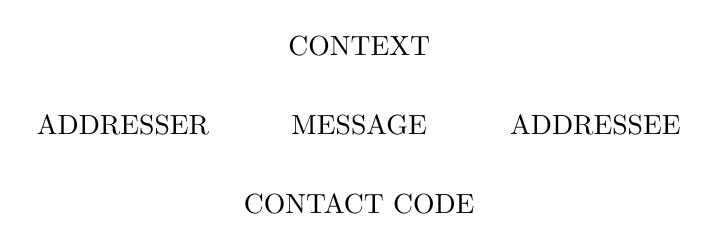
\begin{tikzpicture}
\node(A) at (0,1){ADDRESSER};
\node(B) at (3,0){CONTACT CODE};
\node(C) at (3,1){MESSAGE};
\node(D) at (3,2){CONTEXT};
\node(E) at (6,1){ADDRESSEE};
\end{tikzpicture}
\normalsize

\vspace{-.1cm}
{\it \footnotesize Figure 1: Jakobson's factors of meaning in speech (Jakobson, 2018, p.1070)}
\vspace{0.3cm}

\noindent In every utterance all six factors are present. However, interpretating which factor has the most importance is how the recipient understands the intention of the utterance. Connecting the function with the most important factors we get a schema of the six different ways to use language: 

\vspace{0.3cm}

\small
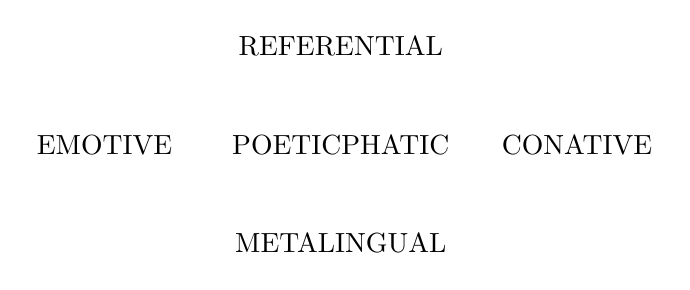
\begin{tikzpicture}
\node(A) at (0,1.25){EMOTIVE};
\node(B) at (3,0){METALINGUAL};
\node(C) at (3,1.25){POETIC \\ PHATIC};
\node(D) at (3,2.5){REFERENTIAL};
\node(E) at (6,1.25){CONATIVE};
\end{tikzpicture}

{\it \footnotesize Figure 2: Six different uses of language (Jakobson,2018, p.1074)}

\vspace{0.3cm}


When the most important factor is the addresser (so the person speaking), the intention behind an utterance becomes \textit{emotive}; that means that what the speaker is feeling or thinking is most important to communicate. Take, for example, the sentence: “It is raining"\footnote{These examples are found\idx{sound} in the lecture on Jakobson by Paul Fry (Fry 2009).}. When the intention is to use this sentence in an emotive way “It is raining” is a dramatic metaphor like one might find in a romantic poem. An expression of sadness and gloom ‘it is raining in my soul.’ The reader or listener must understand this sentence as expressing what the speaker is feeling. 						

When the factor of the addressee becomes cent\idx{scent}ral the \textit{conative} function is most important. This is when the utterance becomes an implicit command, for example a mother seeing her child go outside without a jacket might say “It is raining” meaning a command to put a jacket on. 				
When the utterance is focused on the \textit{context} around\idx{sound} the speakers the function becomes referential. This is when the weatherman says, “It is raining,” merely saying the factual state of the nature around\idx{sound} the speakers. 				

When an utterance is intendent to establish contact (the “Do you hear me?” and “Hello” of language) the function of the speech is \textit{phatic}. Take for example the scene of two awkward young people on a date, both are awkwardly silent and then one of them says “oh, it is raining.” the speaker does not actually care whether it is raining or not, the utterance is simply meant to establish contact. 						
The \textit{metalingual} function is the ability of language to talk about itself. It is Language to correct and explain language. Like how I have been using the sentence “It is raining.” for example but also, questions like ‘what do you mean with “it” when you say, “it is raining?”’ (Actually, a very puzzling question) 							

Lastly there is the \textit{poetic} function, the function that targets the message of an utterance. This might mean the form and rhythm of an utterance or the combination of different concepts in witty similarities. A good example our supervisor Ana gave is: “it is raining bullets.” What is important in the poetic function is the relation between speech and message, the utterance is calling attention to the how and why language works. Instead of selecting the proper word a speaker combines words. Similar to the metalingual function the poetic function focuses of language as a semiotic system. However, the poetic function and metalingual function are in diametrical opposition to each other; the metalanguage function is about how the sequence of words is used to build an equation (‘rain means falling water’ for example) whereas in the poetic function the equation is used to build a sequence (‘look how the shape of the drops of rain resemble bullets’)\footnote{Jakobson explains this with the difficult sentence of : “The poetic function projects the principle of equivalence from the axis of selection into the axis of combination.” (Jakobson 2018:1074)}.

These are the six functions that language has. One way we might get a crystal-clear language is by having the speaker explicitly state that an utterance has one of these six functions. Having a marker to indicate the function. However, besides being very inelegant, that would lead to ridiculous sentences. Besides that, it is an international auxiliary language and was never intended to replace natural languages, merely to work as a tool to easily communicate with speakers with different mother tongues. These functions in language are unavoidable but the aim of Atlan is to make a language that is semantically unambiguous and simple. Atlan, as it is now, is a language whose makeup is heavily tilted to utterances that referent the world as it presents itself for it creates words based on the speaker's empirical data of the world. How people can understand each other in Atlan is though understanding the words as collections of basic axioms, axioms that are experienced in the world. To say “it is raining” in the emotive sense in Atlan you would be better off by arriving to that emotion\idx{emotion} by the emotive axioms of Atlan. Saying “it is raining” in all the different ways as described above clashes with the aim to counter ambiguity in the language. You have to say what you mean to be able to form the words of Atlan. Thus, the language, in the way it forms its words, is always referencing the experience that such a concept entails.   

\section{Culture and Language}


As Max’s introduction already discussed it is difficult to separate culture and worldview from language. Nevertheless, with Atlan we are attempting to do exactly that, in the name of a neutral language. In relation to culture Atlan set out to achieve two things: (1) Atlan needed to be independent to any dominant culture, otherwise it would be no better than English as a neutral lingua franca; (2) cultural expression and lived world needed to be able to be translated into and even be able to be expressed in Atlan. As Max also discussed the relation between language, country, politics and worldview is a very contentious topic and a cause for problems in any auxiliary language. On the one hand, Atlan will need to engage with expression within a specific cultural milieu. But on the other hand, Atlan hopes to be able to evade being tied up to any specific cultural expression as much as that is possible.				 		

We consciously made Atlan as culturally neutral as we could and hoped to give the language enough scope to be able to express all kinds of different worldviews and culturally specific practices and items. It is after all a language that hopes to bridge linguistic and nationalistic divides, this means that it needs to make different culturally specific expression understandable to all speakers. As we have discussed in 7.1previous part Atlan is a language that should focus on the referential use of language. It is a language that tells you the facts as they are for the speaker. This might limit the speaker's cultural expression of the world. What is more important is that people can understand each other, even if that would limit their expressive ability. Here we see why culture is impossible to separate from language; already in Atlan there is a hierarchy of values; comprehension is more important than expressions. 					 

Language without culture is an impossibility and the worldview of its speakers, if language has influence on that, will still be influenced by Atlan just like any other language would do. How Atlan changes its speaker's way of life is evident by its very concept as auxiliary language. To use an auxiliary language a speaker must be open to other cultures and other ways of speaking, especially in our language Atlan. The phonetic of Atlan is such that its speakers need to broaden theirthere understanding of a specific sound\idx{sound} more than their mother tongs would most likely do. Atlan speakers need to be very open and conscientious because words have many ways of being expressed and a concept might be expressed in many different ways. 									 

Consequently, even though Atlan tries to separate language and the sociolinguistic context, it is very questionable that such a thing can be achieved. As the linguist Alvino Fantini argued language and speakers' values, beliefs and attitudes are mutually interdependent. (Fantini 2020) The symbols that make up a language can only be understood in a sociolinguistic context and are interrelated with the worldview and norms, values and beliefs of the speaker. (Fantini 2020:270)		

It is inevitable that Atlan will create its own sociolinguistic context. We might then question whether Atlan is an improvement to a natural language like English as lingua franca. Afterall we had rejected English because it relates to one particular culture and not with all cultures and now it seems that Atlan will only create a new singular milieu: “Two things seem to happen simultaneously: people attempt to fit their language to a situation or context that their language, in turn, helped to create in the first place (Gee qtd. in Kecskes 2008:146).”  				 

This is a problem for Atlan however, it we hope to avoid this problem by making Atlan a very open and lose language. For example, with the phonemes being very flexible and not really having one correct way to say a word. We hope that this creates a culture around\idx{sound} Atlan that is similar to a bilingual or multilingual interaction. What is called by Fantini ‘incipient’ behaviour: 

\begin{quote} 

Simply put, this stresses an attitude of willingness to 	engage with others with no common tongue (not an		uncommon situation) and attempting to communicate. In 	this view, bilingualism begins with attitude, with a 		willingness to engage, even when no skill exists.	(Fantini 273)  

\end{quote} 

Atlan would hopefully create a loose social linguistic milieu that makes it more likely for people from different ethnicities and cultures to try and understand each other. More than if the language would be a natural language like English because in English there is less space for different ways to say something. However, this openness might also be problematic because of the “inescapable Babel\idx{Babel} effect” that we discussed in the introduction of this chapter. More language variation\idx{language variation} will create more confusion. Atlan does not avoid the Babel\idx{Babel} effect, on the contrary, it amplifies it.

\section{Is language grammar\idx{grammar}?}

So far, we have looked at pragmatics\idx{pragmatics} as a source of problems for Atlan. Whether Atlan can express all the functions of language, how pragmatic use confuses Atlan into incomprehensibility, whether orit is not it is impossible to separate language from culture and, lastly, whether language is only meaningful in a sociolinguistic milieu. The pragmatic use of language has been an obstacle to be overcome. The focus was to make a grammatical structure without ambiguities, easy to understand and simple in structure, yet when faced with the task of speaking Atlan it quickly becomes unwieldy and confusing.			 

What my colleagues and I hopedset out to achieve was to create a perfect language first and then see whether people can use it.  We started with the grammar\idx{grammar} and machine algorithms and from there moved on to use. Leaving pragmatics\idx{pragmatics} for the end of the book. It is reasonable to wonder whether this is the best way to understand language. Does language exist without speakers using it? Do the rules of language form the basis for speech or does speech form the basis for the rules of language? The linguist Roy Harris attacks the notion of grammar\idx{grammar} as the basis of language. For him, to understand language, you must place speech/ use first.first. (Haris 1987) Steven Knapp and Benn Michaels Walter take this even further arguing that there is only intention and words, there is no language without speakers. (Knapp and Walter 1985) In other words, a room full of chimpanzees typing at random on typewriters would never create a work of Shakespeare. It could only create a piece of paper with letters on it that look like a work of Shakespeare. A true work of Shakespeare needs to have the intention of an author behind it to be language. These “neo-pragmatic” thinkers show that it is not obvious that we get to a perfect language (or any language at all for that matter) by creating an abstract grammatical structure. 

Many artists and poets are not so sure of our view on language either. The French poet Mallarmé for example rebelled against the notion that things mean what the dictionary says they mean, putting a lot of emphasis on the emotion\idx{emotion} that the sound\idx{sound} of a word invokes. (The French word Jour for example was for Mallarmé to sombre to express “day” and Nuit to joyful.) The futurist project of Zaum is another example; this Zaum ‘language’ has no grammar\idx{grammar} or syntax\idx{syntax} rules and consists of neologisms. It was created by the Russian avant-Garde poets Aleksei Kruchenykh and Velimir Khlebnikov to show that language doesn't dependend on grammatical rules (Tynyanov 1979).						 

That language has an element of what I can only describe as a feel of the language is nicely exemplified in nonsense poetry. Utterance can create significance and meaning even when they should not like in Lewis Carrol’s Jabberwocky (Carrol qtd. in Hofstadter 366):

\begin{quote}
Twas bryllyg, and the slythy toves 
 Did gyre and gymble in the wabe: 
 All mimsy were the borogoves; 
 And the mome raths outgrabe.  
\end{quote}

\noindent Here Lewis Carrol has created a poem mostly made of non-existent words, yet everybody believes that he or she can understand it. ‘It feels right.’ This is also shown in the numerous translation\idx{translation}s made of the poem that reproduce the nonsense words but then in, among others, a French (Frank L. Warrin qtd. In ibid 366) and German (Robert Scott qtd. In ibid 366) setting: 

\begin{quote}
Il brilgue: les t\^{o}ves lubricilleux 
Se gyrent en vrillant dans la guave. 
Enm\^{i}n\'{e}s sont les gougebosqueux 
Et le m\^{o}merade horsgrave.  

Es brillig war. Die schlichten Toven 
Wirrten un wimmelten in Waben 
Uns aller-m\"{u}msige Burggoven 
Die mohmen R\"{a}th’ ausgraben 
\end{quote}

\noindent How then would we be able to translate this poem and linguistic playfulness into Atlan? We cannot. Atlan is too phoneticly flexible, it does not have one specific correct sound\idx{sound} and its words are not ordered around\idx{sound} associations or ‘family resembles’ like in English or French. Pragmatic linguists have a different approach to language than we had when making Atlan. Their understanding of language is shown in linguistic phenomena that Atlan cannot replicate.   

\section{Conclusion}

To sum up, this chapter discussed the pragmatic use of language and what this would entail for Atlan. It discussed how Atlan makes explicit what in natural languages is only implicit, but Atlan can only go that far in incorporating the intentions of speakers into the grammar\idx{grammar}. Furthermore, the chapter engaged with the worry that Atlan’s loose structure will dissipate and confuse the semantic unity of the conlang and that, while Atlan avoids having a dominant culture as much as possible, it does not manage to create a completely culturally neutral language. Besides Atlan also easily becomes confused and splintered because of the high amount of variation in the language. Lastly the chapter engaged with the question whether focusing on perfecting the grammar\idx{grammar} would create a perfect language. Whether the way we created an auxlang  was the correct way. In conclusion then we can say that, while Atlan creates an interesting and potentially rich linguistic experience, the use of the language will pose some problems for its speakers. For one, the language is very phonetically loose, and more effort needs to be exerted when listening to other speakers. Secondly implicit messages need to be made explicitly which creates a peculiar way of thinking that might be frustrating. Lastly, because of its focus on a perfect grammar\idx{grammar}, errors or mispronunciations would quickly cause confusion between speakers. Thus, it is highly doubtful whether Atlan will be able to reach its goals when pragmatically used.  This does not mean that Atlan is  a failure, far from it. The set of words that we have created is interesting as a poetic project. Being the average human sound\idx{sound} of one particular semantic meaning, a word in Atlan shows what one particular sound\idx{sound} means for the collective average human being. Atlan is a project that shows how meaning can be created and shared from very basic human experiences.  Communication might be blocked by language barriers; language will carry meaning for everybody who meaningfully listens. Although much is still to be discovered, and much more needs to be thought about to make Atlan a complete language, Atlan has created a system to make elegant and meaningful words from fundamental human life-experience. We now hope that more people will get excited about this project and help co-create Atlan on a daily basis. What Atlan misses most is speakers, people who can live in and express themself in Atlan. Hopefully we can find many of such co-creators.



\chapter{Further suggestions}



\section{Sign Language -- {\small Stijn Janssens}}
According to the World Health Organisation, anno 2015, some 5\% of the world’s population is deaf. Different countries have their own sign languages, but these are often mutually unintelligible. Currently, no standard universal sign language exists. In our project, we did not focus our attention on creating a sign language to accompany Atlan as an IAL, but we might suggest how others, who have more knowledgeable on this topic than us, might use Atlan to construct such a sign language. 

A database of signs from different sign languages might be used, such as ‘Spreadthesign’ by the European Sign Language Centre. Software such as Sign Language Processing (SLP) might be used to build data models to formalize and compare signs from different languages. This way, ‘universal’ signs might be generated by identifying overlap or similarity in signs between language, weighing each language by relatedness and amount of speakers. These could then be mapped onto Atlan’s lexicon, and from there the whole language might be essentially copied into this sign language.  

Having such a signing system might have the benefit of allowing deaf people from around the word to communicate with one another. It might also make sign language more accessible to hearing people, who would only have to learn some 490 signs, provided they already speak Atlan. This would foster communication and mutual understanding between deaf and hearing people, as well as serving as an extra linguistic gadget for communication when two speakers can see each other, while unable to hear what the other is saying due to whatever circumstances. 

\section{Language Variation -- {\small Niek Elsinga}}

Imagine yourself in the following situation: You are standing in front of a machine which will take you back in time to the year 1223, 800 years in the past. Peace had just returned to England after a hard-fought civil war which resulted in the signing of the Magna Carta, which limited the power of the English kings. England in this time was a country that was still full of meadows, forests, and pristine nature, with a relatively small population of an estimated 4 million people, nearly 60 million fewer than today. You would be able to walk around, and enjoy a moment of tranquillity, peace, and quiet along crudely constructed cobbled walls which indicated roads that led to small villages, towns, and cities. While these towns might have been humble and quaint, they still bustled with life. People buzzing in tightly cramped avenues, with the smells of fresh crisp sourdough bread, savoury stews brewing above campfires, and the pungent aromas of leather tanners, and the fires of the bellows of blacksmiths must have all coalesced in the cacophony of the community. Shops, pubs, and artisanal boutiques which sell clothes and other food stuffs are able to be found in dimly-lit alleyways. Market stalls with several kinds of fruits, vegetables, loaves of bread, meat, and perhaps even a mystic stall with unique herbs and spices from a faraway land are able to be found on plaza on a Saturday morning. 

You walk up to a stall which sells different types of stew. While you are not entirely certain what it is in it, you are drawn to a certain type of stew which is simmering above a fire. Its aromas and smells are unlike you have seen thus far, and thus, you go ahead and order a portion of this seemingly tasteful concoction. “I would like to order a portion of this stew, please,” you would say. The salesman looks you in the eye, astounded and, perhaps, suspiciously. He replies: “Hwæne canst þú ġecwides?” You look dumbfounded at the vendor. With every single word that you try to pronounce, it seems that his gaze turns more hostile. Eventually, you just point. “That one, please,” whilst pointing to a stew you did not even examine. You give him the money, which he luckily accepts, and hands you a bowl full of the other substance. This one smells significantly less refined than the other one, but you cannot be bothered to go back and voice your dissatisfaction. It was your fault either way, since you pointed erroneously. You sigh, and begrudgingly eat your stew which still turns out to be somewhat alright. 

 

What happened here? How come that you were not able to understand each other? In this case, there are two factors to this. First and foremost, language changes and branches out over time. This is normal, natural, and occurs organically. Because of language change, the Vulgar Latin of the Roman empire diverged and evolved into the modern Romance languages of Spanish, Portuguese, French, Italian, over the course of the last two millennia (Sala \& Posner, 1999). The same happened with Vedic Sanskrit, which is the now-extinct language from which a plethora of languages on the Indian subcontinent are derived from (Burde, 2004). 

The second factor is a variable that has happened in the English language specifically, which is a shift in the pronunciation of English vowels. The standardization of the English script occurred between the 15th and the 16th centuries (Denham \& Lobeck, 2009), while the pronunciation of English vowels shifted during this time. This shifting-event occurred between the 15th and 18th centuries, and influenced the pronunciation of vowels of every single English dialect (Labov, 1997). Where the vowels in the word “boot” are currently pronounced akin to the Dutch diphthong /oe/ in “koe”, or just the standard English [oo], in the 13th century it would have sounded more like the Dutch /oː/ as in “groot”, or the $\langle$aw$\rangle$\footnotemark in the modern British English word “yawn”. This Great Vowel Shift (GVS), as it is called, resulted in a different pronunciation compared to the graphemic notation for the entirety of the English language (Denham \& Lobeck, 2009). 

\footnotetext{These brackets are used for linguistic notations. $\langle\ldots\rangle$ is used for graphemic notation (i.e., the letters as they are written down); [...] is used for the actual realized phoneme (i.e., the sound that is actually created); and /.../ is used for the intended phoneme.}

The GVS likely occurred because of multiple reasons, however, there is no academic consensus for one single solution (Silverman \& Silverman, 2012). Some theories include migrations towards the southeast of England from neighbouring regions following the population decline caused by the Black Death (Crystal, 2018). Another theory is the influx of French loanwords with differing pronunciation compared to the Anglo-Saxon pronunciation of Old and Early Middle English (Millward \& Hayes, 2011). Another theory is the complete opposite, which states that due to the wars with France in which England was entangled at that period in time, anti-French sentiment caused a shift in pronunciation to make English phonemes sound less French (Nevalainen \& Traugott, 2012). It is more likely that the GVS occurred due a combination of these factors, rather than that a single one resulted in the entirety of the changes (Silverman \& Silverman, 2012). 

Nonetheless, it occurred, and English has not been the same since. It is not unlikely that events like the GVS will happen again since language is fluid per definition. Scholars agree on that language variation and change is both inevitable, unpreventable, and continuously happening (Lyons, 1968). In this essay, I will elaborate on the specifics of language change, how it can occur, and how we have designed our language to be resistant to language variation and change to a certain degree. 


\subsection{Language variation and change: inevitable?}

Language variation refers to the different ways in which a language can vary based on factors such as geography, social groups, historical periods, and individual speakers. These variations can manifest in various forms, including pronunciation, vocabulary, grammar, and usage (O’Grady et al., 2001). Take regional dialects, for example. Different regions within a country or even different countries that share the same language may have distinct dialects. For instance, in Dutch, there are variations between the Dutch from the Netherlands and the Dutch from Flanders. These dialects can diverge in pronunciation (e.g., the pronunciation of the letter “g” and “r” in the Netherlands and Flanders (Verhoeven, 2005)), vocabulary (e.g., the use of the second-person pronoun “uw” in Flemish contrasted with “jouw” in Dutch (Vandekerckhove, 2005)), and grammar (e.g., “moeten aan doen” in Flemish compared to “aan moeten doen” in Dutch (Haeseryn, 1990)). Another example is sociolects, which are variations based on social factors such as social class, education level, or occupation. There may be differences in vocabulary and speech patterns between a group of doctors and a group of construction workers, reflecting their professional backgrounds and the jargon they use in their respective fields (Bybee, 2015; O’Grady et al., 2001) 

The main point in language variation is that variation is not the same as language change, however, language variation often does serve as a precursor to language change (Chambers et al., 2004). When a language exhibits variation among its speakers or regions, it provides the foundation for changes to occur and spread throughout a language community. Language change, in continuation of language variation, refers to the process by which a language undergoes modifications over time. There are multiple factors about language change, which can occur at every linguistic level: Phonology and phonetics, morphology, syntax, semantics, and pragmatics (Meecham \& Rees-Miller, 2001). Phonological change involves alterations in the sounds of a language. Over time, sounds can shift in pronunciation, merge with other sounds, or split into distinct sounds. This happens more frequently if multiple sounds exist which sound similar, such as the /$\theta$/ in $\langle$ thing$\rangle$ being replaced by the /f/. This happened to me personally, and occasionally I still make the error of pronouncing the $\langle$th$\rangle$ as an /f/ instead of the /$\theta$/. Lexical change refers to changes in vocabulary. New words are constantly introduced into a language, while others become obsolete or change in meaning. For instance, the word “awful” originally meant “full of awe”, but has shifted to its current meaning of “bad” or "terrible" over time (“Awful, Adj. and Adv.: Oxford English Dictionary,” n.d.). Languages can also undergo changes in their grammatical structures. This includes modifications in verb conjugation, word order, and the use of grammatical markers. Take for example the distinction with the indirect object “aan” in the Flemish “moeten aan doen” compared to the Dutch “aan moeten doen”, as stated earlier (Haeseryn, 1990). Semantic change occurs when the meaning of words or phrases evolves over time. Words can acquire new meanings, lose old meanings, or sustain shifts in connotation. An example is the word “gay”, which originally meant “happy” but has taken on the additional meaning of “homosexual” in modern usage (Hiskey, 2015). 

\subsection{Variation, change, and its mechanics}

Besides changes in language as part of coincidences of linguistic levels, change can also be instigated by social factors such as group identity and language contact. Social factors play a crucial role in shaping language variation and driving language change. Certain speech styles or dialects may be associated with social prestige, power, or higher social status. Speakers who want to align themselves with certain social classes may adopt features associated with these groups. Take for example the use of certain lexical items, jargon, or words on a semantic level. Using words associated with the desired group can give the illusion of being associated with said groups. As a result, language change can occur as features from prestigious or standard varieties are adopted and incorporated into the speech of a wider population (Labov, 1990). Besides class and income, speakers may also associate themselves with certain social groups, such as skaters, punks, emo’s, etc. Language is an important marker of social identity. Speakers may consciously or unconsciously modify their language use to identify with or differentiate themselves from particular social groups. Language change can occur as speakers apply features of the identity of the target group as a way to signal membership in a specific community or subculture. This happens oftentimes in groups of young adults, and as such, older individuals might not understand them (Coupland, 1985). Language change is also often observed between different generations. Younger speakers may introduce new linguistic innovations or modifications in their language use compared to older generations. Over time, as younger generations become the majority, their linguistic features may spread and become more widespread, leading to language change (Kerswill, 1996). However, within these older populations, language change can occur as well, through social networks. Perhaps some elderly individuals create a certain lect during their poker-games. Because speakers interact with others in their social networks, language change can be achieved through the innovation and diffusion of these linguistic innovations. Language change can occur when innovative linguistic features spread through social networks, especially if influential individuals or groups adopt and promote these features (Ke et al., 2008). More sinister causes of language changes can also occur. If a particular variation is stigmatized or associated with negative stereotypes, speakers may avoid using those features or modify their language use to conform to more prestigious or socially acceptable forms (Maass, 1999). The opposite can also occur, in that positive attitudes towards certain features can promote their adoption and spread, leading to language change. This strikes back at the aforementioned options. 

\subsection{Implications for Atlan in language development}

There are many reasons for both language variation and language change. Change and variation in language are inevitable (Aitchison, 1994). How does this fare against constructed languages then? Very few constructed languages have seen wide-spread implementations, or mass numbers of speakers. It seems that there is limited evidence for linguistic variation in Esperanto, the major constructed language (Sherwood, 1982). However, Sherwood (1982) solely found variation in the pronunciation of phonemes, and there was still no mutual unintelligibility whatsoever. This is also likely due to the fact that Esperanto has seen no official adoption globally, and its use is mostly by aficionados (Piron, 1989). This causes the spoken language to be more or less the same as when it was invented, approximately 150 years ago. 

Treading the waters of future language variation can be a difficult subject, due to the fact that the future, simply put, cannot be predicted. Language variation and change is, of course, inevitable. However, we have taken steps in order to make Atlan more resistant to language change. This is mostly centred in the phonology: because there are cardinal groups for both vowels and consonants in which similar phonemes are both allophonic and grouped, variation will less likely occur on a phonemic level. The same is the case for morpho-syntax because prepositions, referents, demonstratives, etc. all have a fixed set and meaning, and syntaxial variation is allowed to a certain degree. Furthermore, because the lexicon is procedurally generated, but random by definition for other items, variation is more likely to occur due to the implementation of lexical items of the mother tongue of a speaker. This so- called L1-to-L2-transfer (Sparks et al., 2009), however, is a feature of Atlan. Because some lexical elements and words with complex meanings cannot be accurately translated due to cultural differences (House, 2010), speakers are encouraged to translate it literally, and perhaps elaborate on it to unknowing speakers. A good example of a word that has no direct literal translation in English is the German word ‘Schadenfreude’. In Atlan, this word could be described as “joy (SUS \sus) + other (OF \of) + affect (SIN \Atlansin) + bad (PAK \pak) = SUS.OF.SIN.PAK” \sus \of \Atlansin \pak. The use of these lemmas implies that a negative occurrence caused another person, in this case the person speaking it, a certain degree of joy. By describing the source word in Atlan, it can be understood by a wider array of speakers who are not familiar with the term. Variation in this case then is more or less irrelevant unless the words themselves change meaning. However, because the lemmas are procedurally generated, variation can only occur if a pronunciation of a consonant or vowel is changed. And this, of course, is less likely due to the grouping of the consonants and vowels in their allophonic categories. Due to these considerations, we think that Atlan as a whole will likely experience a delayed progression of variation and change.

\subsection{Conclusion}

If anything is clear, it would be that language variation and change is inevitable, unpredictable in its course, and constantly occurring. Atlan, like every other language, will meet the same fate, and changes will occur, be it regionally, socio-economically, age or culture-related. Perhaps in the future, multiple different variations of Atlan will coexist, intelligible or unintelligible. Then, the decisions made for the mitigation of language variation and change will be in vain. However, is that not exciting? When language variation occurs, this means that it is alive and fluid. Being able to see a language flourish is, perhaps, a better outcome than rigid measures intended to keep the language intelligible for everyone.




\chapter{Example texts}
\section{The Story of Babel -- {\small Jonathan Roose}}

1 Everybody		on 	Earth 		had

ALL.PERSON.PLURAL   	ON(AF)	ALL.PL-EARTH	PAST.BE	 

AT.EI.ON		AF	AT.TEM		PA.SI	 

ateion		\af	\at\tem		\pa\si	 

\vspace{0.2cm}

the same language	 and 	the same words. 

ACC.ONE.SAY.COMU.	AND.	ACC.SAME.WORD.PLURAL 

EK.IP.(A).LAN.SUM	AN	EK.ME.SET.ON

\vspace{0.5cm}

2 And	 		it came to pass, 			  

REL-CLAUSE.AND            AT.TIME.THIS.PAST.HAPPEN.		

I.AN			ET.JA.ES.PA.NES				 

\Atlani\an                    \et\ja\es\pa\nes

\def\drie{\vspace{0.3cm}}
\drie

as	they	    

REL-CLAUSE.PROGR.TIME	THR.PERS.PLURAL 

%\I\PO\JA	\AJ\ON 


migrated          			from      		 VERB.MOVE.PLACE.HOME	DIRECTION.ORIGIN	 

TU.MEF.LU.KEM			LI.JOL 

 

the east, 		They 		 

PLACE.BIRTH.SON	3TH-REMO.PLURAL 

LU.PES.SON		AJ.ON 

  

came upon 		a valley                 

PERFECTED.ECOUNTER  	ACC.PLAIN.BETWEEN.MOUNTAIN.	NI.FAF                                EK.PAS.MI.MAN 

  

in the land          of Shinar 

AT.COUNTRY	PLACE.NAME.[SHINAR] 

ET.MES		LU.NA.[S.JI.NAR] 

  

And 	they 		settled			 

AND.	3TH.PLURAL	VERB.MAKE.SIT.HOME	 

AN	AJ.ON		TU.MEN.SUP.KEN 

  

There.			₃ they		said 	 

DEMONST.2ND.PLACE	3TH.PLURAL	PAST.SAY 

ES.AJ.LU		AJ.ON		PA.LAN	 

  

to one another, 			 

DATI.SELF.OTHER.PLURAL		 

LO.SU.OF.ON 

  

“come, let us make   

IMPERATIVE.VERB.MAKE.1ST.REMOVED.PLURAL 

0.TU.MEN.AM.ON 

 

bricks				And 	 

ACC.BUILD-BLOCK.STONE.PLU 	AND		 

EK.FUK.JET.ON			AN 

  

burn them			hard” 

CAUSE.BURN 			DEMOSTRATIVE.BECOME.SOLID 

KO.PEN				ES.PIN.TOJ				 

Bricks 				served 				 

BUILD-BLOCK.STONE.PLUR          VERB.FINAL-STATE.PREDICATE	 

FUK.JET.ON			TU.FU.SI			 

Them			as 	stone	 

DAT.3TH-PERSON.PLUR AS	BUILDING.MATTER.STONE. 

LO.AJ.ON		ME	FUK.MAJ.JET 

  

and	bitumum 		served  

AND	PETRO.NA[BITUMUM]	TU.FINAL-STATE.PREDICATE 

AN	PAT.NA[BI.TU.MUM]	TU.FU.SI 

  

Them				as 	mortar 

DATI.3TH-PERSON.PLUR               AS	BUILDING.MATTER.FOAM 

LO.AJ.ON			ME	FUK.MAJ.MOP 

  

₄ And 			they 				said  

RELA-CLAUSE.AND          PERSONS.3TH-REMO.PLURAL 	PAST.SAY 

I.AN			EJ.AJ.ON			PA.LAN 

  

“come, let us build                                                                          

IMPERATIVE.VERB.MAKE. BUILDING.1ST.REMOVED.PLURAL	 

0.TU.MEN.NAP.AM.ON                                                                              

 

a city			And 	a tower	 

ACC.ONE.TOWN		AND	ACC.BUILDING.LONG.VERTICAL 

EK.IP.TOS		AN	EK.NAP.LAK.TE	 

 

with its top 				in           the sky 

GENA.THIS.3TH-REMO.ABOVE.PART	IN	SKY 

TA.ES.AJ.EF.PU				IN	SOM 

  

To make 	a name 		for ourselves		 

VERB.MAKE	ACC.NA		DAT.1ST-REMO.PLURAL	 

TU.MEN	EK.NA		LO.AM.ON 

 

else 			we 

OTHER.POSSIBLE	1ST-REMO.PLURAL 

OF.PI			AM.ON 

 

shall be			    scattered			PROGRESIVE.PRESICATE    VERB.PREDICATE.NEGATION.ONE        

PO.SI			     TU.SI.NE.IP		 

 

all over			The earth 

NEAR.AND.FAR		ROUND.PLAN-EARTH 

KI.AN.FA		LOK.TEM 

 

₅ the LORD 		came down 			EXCLAMATIVE.GOD         VERB.PAST.COME.DOWN		O.JEL			TU.PA.KOM.LIT			 

 

to look			at the city 

DESIRE.VERB.SEE	ACC.CITY 

FAN.TU.SIK		EK.TOS 

  

And 	tower 				that 			 

AND	ACC.BUILDING.LONG.VERTICAL	DEMONSTRATIVE	 

AN	EK.NAP.LAK.TE			ES			 

 

Men				had built 

COMMUNITY.PERSON.PLURAL	PERFECTED.MAKE.BUILDING 

EJ.SUM.ON			PO.KEN.NAP 

  

₆ and 			the LORD            said 

RELA-CLAU.AND              EXCLA.GOD	PAST.SAY 

I.AN			O.JEL		PA.LAN 

  

“if, 			as one people 				CONDITION	POSSIBLE.ALL.ONE.COMMUNITY		 

IF			PE.AT.IP.SUM				 

 

with one language 		for all, 

INSTRU.ONE.SAY.COMMUNITY	GENA.3TH-REMO.ALL.PERSON	 

UT.IP.LAN.SUM			TA.AJ.AT.EJ 

 

this is 				how       	they  

1ST-RELA.DEMONSTR.PRED.	VERB.INSTRU.    3TH-REMO.PLURAL 

AM.ES.SI			TU.UT		AJ.ON 

  

have begon 			to act		then 		 

PERFECTED.BEGINNIN.                 VERB.CUSTOM	CONC.CONTR	 

NI.KA				TU.KUK		IS.KU                     

nothing 	that		They 	 

PREDAC.OR	DEMONSTRA.	3TH-REMO.PLURAL 

IS.OL		ES		AJ.ON	 

 

may propose			to do		will be 

VERB.SAY.POSSIBL.IMAGI	FUTR.VERB	FUTR.PREDICATE 

TU.LAN.PI.NIL		               FI.TU		FI.SI 

  

Out 		of their 				reach 

OUTSIDE	GENI.3TH-REMO.PLURAL	META.RANGE.HAND 

AP		TA.AJ.ON			MU.TO.JAM 

  

₇ let us, then, go down, 			      	 

1ST-REMO.PLURAL CONCLU EXCLA.INTENT.GO.TOWAR.DOWN             

AM.ON	IS	 O-UF.MEF.LI.OT				 

 

and  			Confound 

RELA-CLAU.AND	VERB.DISSOCIATION.KNOW.THINK 

I.AN			TU.LIS.NEF.SIN      

  

their 			speech				GEN.3TH.PLURAL             ACC.SAME.WORD.PLURAL	 	TA.AJ.ON		EK.ME.SET.ON 

  

There			so 			they 		DEMONSTR.3TH.PLACE        INTENT.		3TH.PLUR	 

ES.AJ.LI				UF		AJ.ON				 

shall not understand 		One another’s 

FUTR.NEG.KNOW.THINK		ACC.SELF.OTHER.PLURAL 

FE.NE.NEF.SIM			SU.EK.OF.ON	 

  

Speech 

ACC.SAME.WORD.PLURAL 

EK.ME.SET.ON 

 

₈ thus 		the LORD 					CONCLU.	EXCLA.GOD					 

IS		O.JEL		 

 

scattered				them 

VERB.PAST.PREDICATE.NEGATION.ONE	ACC.3TH.PLUR 

TU.PA.SI.NE.IP				EK.AJ.ON 

 

From 			there 			over 		DIRECTION.ORIGIN         DEMONSTR.3TH.PLACE  NEAR.AND.FAR 

LI.JOL			ES.AJ.LU		KI.AN.FA	 

 

 

the face of the whole earth 

ACC.ALL.SURFICE.PLAN-EARTH 

EK.AT.SEM.TEM 

 

And 	they 		stopped 				 

AND	3TH.PLUR	VERB.NEG.COMPA.TRANS.HAPPEN	 

AN	AJ.ON		TU.NE.MO.NES		                               

 

building 		the city 

VERB.MAKE.BUILD	TOWN 

TU.KEN.NAP                      TOS 

 

₉ That is way 				it 			DEMONSTR.REASEN.PREDACITE	ACC.STRESS.CITY	 

ES.KO.SI				EK.A.TOS		 

 

was called Babel 

VERB.PAST.NAME[BABEL] 

TU.PA.NA[BA.BEL] 

  

Because 		there 				the LORD  

REASON.FIN-STATE          DEMOSTR.3TH.PLACE		EXCLA.GOD 

KO.FU			ES.AJ.LU			O.JEL 

  

Confounded 

VERB.PAST.DISSOCIATION.KNOW.THINK	 

TU.PA.LIS.NEF.SIN                                               			 

 

The speech			 of the whole earth 

ACC.SAME.WORD.PLURAL 	ALL.PLA-EARTH.COM. 

AT.TEM.SUM			EK.ME.SET.ON 

 

And 			from 			there 		RELA-CLAU.AND	DERECTIO.ORIGIO      DEMONSTR.3TH.PLACE 

I.AN			LI.MI			ES.AJ.LU			 

the LORD	Scattered 

EXCLA.GOD	VERB.PAST.PREDICATE.NEGATION.ONE 

O.JEL		TU.PA.SI.NE.IP    

 

 them 		over 		 

ACC.3TH.PLUR	NEAR.AND.FAR	 

EK.AJ.ON	KI.AN.FA               

  

the face of the whole earth. 

ACC.ALL.SURFICE.PLAN-EARTH 

EK.AT.SEM.TEM 



\section{The Epic of Gilgamesh -- {\small Niek Elsinga}}


Enkidu’s Dream 

 
 

With these last words the dying Enkidu did pray, and say to his beloved companion:  
 [ENKITU].SI.PO.MOT TU.PO.LAN.LO.JEL ES.NI.SET.ON, AN LAN EK.LO.LUF.TEN 

\{ENKITU-predicate-process-death\} \{verb-process-speak-to-God\} \{with this word word\}, \{to\} \{speak\} \{accusative-to-love-acquaintance\} 

 
 

"In dreams last night | the heavens and the earth poured out great groans while I alone stood facing devastation.  

ET.SUL.ON.TAN SOM.ON AN TEM TU.NI.KOL.MAJ EK.PIK.LAN.SIN.PAK PO.JA SU NE.SUM PA.TUF TU.TA.JUN 

\{location-dream-plural-hallucination\} \{sky-plural\} \{and\} \{earth\} \{verb-perfective fall matter\} \{accusative augmentative say affect bad\} \{progressive time\} \{self\} \{negation-community\} \{past stand\} \{verb genitive destruction\} 

 
 

A fierce and threatening creature flew down at me and pushed me with its talons toward the horror-filled house of death wherein lrkalla, queen of shades, stands in command.  

TUT AN TEF.TU.MEN NIK TU.PA.FUL.ET.OT LI.AM AN TU.PA.AJ.PUS.AM AN AJ TA.TAK.NEK.ON ET TEF.MOL.NAP.MOT LU [IR.KAL.LA] FI.TES.PU.NE.SON.LAS AJ.TUF.IN.TA.O 

\{strong\} \{and\} \{fear verb creation\} \{creature\} \{verb past fly coordinate under\} \{direction 1SG\} \{and\} \{verb past 3SG push 1SG\} \{and\} \{3SG\} \{genitive sharp nail plural\} \{coordinate\} \{fear full house death\} \{cartouche name\} \{feminine king-of-negation sun light\} \{3SG stand in genitive imperative\} 

 
 

There is darkness which lets no person again see light of day.  
 ES.AJ SI NE.LAS ES O NE.EJ TU.SIK LAS.PU.JAN 
 \{demonstrative 3SG\} \{is\} \{negation light\} \{demonstrative\} \{imperative\} \{negation person\} \{verb see\} \{light of day\} 

 
 

There is a road leading away from bright and lively life.  
 ES.AJ SI LOL.LI.LU.NE.AM.ES.LU PU LAS AN SUS FIN 

\{demonstrative 3SG\} \{is\} \{road direction place negation 1SG demonstrative place\} \{from\} \{light\} \{and\} \{joy\} \{life\} 

 
 

There dwell those who eat dry dust and have no cooling water for their awful thirst.  
 ES.AJ LU.PUJ ES.AJ.EJ EK.EJ TU.KOS.TOJ SUK TUL AN TU.NE.TA MEK.TEP.NET TU.KOS.JIT SUK.MUT 

\{demonstrative 3SG\} \{place stay\} \{demonstrative 3SG person\} \{accusative person\} \{VERB consume solid\} \{dry\} \{dust\} \{and\} \{verb negation genitive\} \{low temperature water\} \{verb consume liquid\} \{dry mouth\} 

 
 

 
 

As I stood there I saw all those who've died and even kings among those darkened souls have none of their remote and former glory. 
 IN.JA SU TU.PA.AM.TUF ES.AJ SU AT ES.AJ.EJ TU.TA.EJ TU.PA.MOT AN I.O.ME TES.ON MI.AJ ES.AJ.EJ TU.PO.NE.LAS MAK.ON TU.NE.TA TA.AJ LU.FA AN POP JEJ 

\{inside time\} \{self\} \{verb past 1SG stand\} \{demonstrative 3SG\} \{self\} \{all\} \{demonstrative 3SG person\} \{verb genitive person\} \{verb past death\} \{and\} \{imperative exclamative equivalent\} \{king plural\} \{in-between 3SG\} \{demonstrative 3SG person\} \{verb progressive negation light\} \{mind plural\} \{genitive 3SG\} \{place far\} \{and\} \{previous\} \{success\} 

 
 

All earthly greatness was forfeit and I entered then into the house of death.  
 AT TA.KU.PIK.FO.TEM TU.PA.SI AN SU TU.PA.IN.TOM EK.IN.NAP.MOT 

\{all\} \{genitive comparative big positive earth\} \{verb past is\} \{and\} \{self\} \{verb past inside walk\} \{accusative inside house death\} 

 
 

Others who’ve been there long did rise to welcome me." 

OF.ON ES.AJ.EJ OF.AM.LU LAK.JA TU.MAL.LU 

\{other plural\} \{demonstrative 3SG person\} \{other 1SG place\} \{long time\} \{verb greet place\} 






\chapter{Exercises -- {\small Max Geraedts}} 

The purpose of these exercises is to make the reader familiar with Atlan. To get a feel for the language. They should not be seen as a test of the knowledge of the reader but rather as a guide to get your bearings in Atlan.  


\noindent \textbf{Exercise 10.1 -- Creating a basic possessive sentence \& writing your own name} 

In this first exercise we will be translating the sentence “My name is …" this exercise will demonstrate how to combine words in Atlan to create new words in a simple and familiar context. 

We will start by creating the Atlan word for “my”. To help you along I will give you the Atlan translation\idx{translation} for “I”; EJ.AM \ej\am. “I” is composed of EJ \ej meaning person, and AM \am; 1st removed: speaker. The Atlan word for “my” can easily be made from this by adding the possessive prefix TA \ta. This leaves us with TA.EJ.AM \ta\ej\am.  

And what is the Atlan translation\idx{translation} of “name”? And “is”? (Note: “is” is a predicate and comes with a marker). Remember that the subject of an Atlan word always comes first in a sentence, so the word order\idx{word order} would be: Name my is [Name]. 

Now comes the easiest part of the sentence, your name. To write your name in Atlan all you must do is transliterate your name into Atlan’s set of 14 sound\idx{sound}s and put a cartouche\idx{cartouche} around  your name. %Now, what would be the Atlan translation\idx{translation}s of “My name is …"? 
\begin{itemize}
	\item[(i)] Write your name in Atlan:
	\vspace{0.3cm}
	\dotfill
\end{itemize}

\noindent \textbf{Exercise 10.2 -- Creating basic active sentences in the present simple tense} 

Now that we know how to create a basic possessive sentence, we are going to look at how to form basic active sentences. Like, “I am walking” and “He is writing”.  
\begin{itemize}
\item[(i)] What is the Atlan translation\idx{translation} for “I walk”, “You walk” and “He walks”? (Note: present tense has no need for a marker).  
\end{itemize}

\noindent And what is the English translation\idx{translation} of the following sentences? 
\begin{itemize}
    \item[(ii)] EJ.AM TU.LIK EK.POK \ej\am \tu\lik \ek\pok  

    \item[(iii)] EJ.AJ TU.JIL EK.FIL\ej\aj \tu\jil \ek\fil  

    \item[(iv)] EJ.AM.ON TU.KOS.TOJ \ej\am\on \tu\kos\toj 
\end{itemize}

\noindent \textbf{Exercise 10.3 -- Creating basic sentences in the past simple tense} 

Now we move to the past simple tense. Translate the following English sentences to Atlan. 
\begin{itemize}
    \item[(i)]I worked. 

    \item[(ii)]We worked. 

    \item[(iii)]They worked. 

    \item[(iv)]You played yesterday. 
\end{itemize}
 

\noindent \textbf{Exercise 10.4 -- Numbers} 

Atlan’ number system can be used as a ten-base system and as a twelve-base system. To see the difference between these systems you can look at how to spell your name in both ten-base and twelve-base. We will begin with exercises that use the ten-base system as this will probably be more familiar. 

\noindent Translate the following sentences using a ten-base number system:

\phantom{.}\\

\begin{itemize}
    \item[(i)]I have three fish. 

    \item[(ii)]I have eleven fish. 

    \item[(iii)]I have a thousand fish. 
\end{itemize}
\noindent Translate the following sentences using a duodecimal\idx{duodecimal} (twelve-base) number system:
\begin{itemize}
    \item[(iv)]I have three fish. 

    \item[(v)]I have eleven fish. 

    \item[(vi)]I have a thousand fish. 

    \item[(vii)]I have a 1.728 fish.  
\end{itemize}
 

\vfill 
\pagebreak
 

 

\section{Solutions}
\small

\noindent{\bf 10.1} -  “My name is …" in Atlan would be; NA TA.EJ.AM SI [NAME] \na \ta\ej\am \si \cartouche{NAME}. 

 

\noindent{\bf 10.2}
\begin{itemize}
    \item[(i)]I walk = AM.TU.TOM \am\tu\tom 

    \item[(ii)]You walk = UN.TU.TOM \un\tu\tom 

    \item[(iii])He walks = AJ.TU.TOM \aj\tu\tom 
\end{itemize}
 

    %EJ.AM TU.LIK EK.POK \ej\am \tu\lik \ek\pok = I write a book. 
    %EK \ek indicates that POK \pok is the object of the sentence. 

    %EJ.AJ TU.JIL EK.FIL\ej\aj \tu\jil \ek\fil = He drives a vehicle. 

    %EJ.AM.ON TU.KOS.TOJ \ej\am\on \tu\kos\toj= We eat. 
    %\on indicates that \am is plural making it “we” instead of “I”. \kos (consume) combined with \toj (solid) means eat. 

\noindent {\bf 10.3}
\begin{itemize}
    \item[(i)]  EJ.AM PA.TU.KAN \ej\am \pa\tu\kan 

    \item[(ii)] EJ.AM.ON PA.TU.KAN \ej\am\on \pa\tu\kan 

    \item[(iii)]EN.AJ.ON PA.TU.KAN \ej\aj\on \pa\tu\kan 

    \item[(iv)]EJ.UN.ON PA.TU.LAJ ET.JAN.POP 
\item[] \ej\un\on \pa\tu\laj  \et\jan\pop 
\end{itemize}

\noindent \textbf{10.3.4 Numbers} 
\begin{itemize}
    \item[(i)]EJ.AM TU.TA MIS.UP - \ej\am \tu\ta \mis\up 

    \item[(ii)]EJ.AM TU.TA MIS.JI.IP - \ej\am \tu\ta \mis\ji\ip 

    \item[(iii)]EJ.AM TU.TA MIS.NU - \ej\am \tu\ta \mis\Atlannu 

\item[(iv)] EJ.AM TU.TA MIS.UP  - \ej\am \tu\ta \mis\up 

    \item[(v)] EJ.AM TU.TA MIS.JO - \ej\am \tu\ta \mis\jo 

    \item[(vi)] EJ.AM TU.TA. MIS.UK.JO.IK 

\item[]\ej\am \tu\ta \mis\uk\jo\ik 

    \item[(vii)] EJ.AM TU.TA MIS.NU \ej\am \tu\ta \mis\Atlannu
\end{itemize}

%%%%%%%%%%%%%%%%%%%%%%%%%%%%%%%%Endmatter%%%%%%%%%%%%%%%%%%%%%%%%%%%%%%
\backmatter

\chapter{Epilogue}\section{Special Thanks}

Special thanks to, 

{\bf Ana Bosnic}¸ for her amazing guidance throughout this whole book. Ana, we wouldn’t know where would be without you. 

We vividly remember how badly we wanted you to be our supervisor. Luckily, your enthusiasm for this project was almost bigger than ours! You always had great ideas and was ready to help. We cannot thank you enough for all the proofreading you did and your many (!) comments. Your constructive criticism and thoughtful suggestions brought the quality of our book to a whole new level. Your insights and expertise added depth and credibility to our work, and we couldn’t be more grateful.  

Also, thank you for putting up with our chaotic meetings, late notifications, and last-minute room changes. You never gave up on us: even if there had to be three separate meetings to let all of use view one documentary. Your commitment and perseverance made all the difference, and we are sincerely grateful for your support. 

Ana, we had a total blast these couple of weeks! Since you will not give this course anymore, we surely hope it was just as much fun for you! Thank you a million times over! 

  

Angela Carpenter, for her support and contribution to this project. Angela, your help and assistance have truly made an impact on this product.  

That afternoon when you were ready to lend an ear, despite the crazy time difference, was a true joy for us. How cool it was that we were talking with the professor we saw in a documentary only a few weeks before! Your patience and genuine interest in our non-existing language made our brainstorming session truly delightful. We owe you a debt of gratitude for sharing all that knowledge from your classes. Your enthusiasm, and encouragement meant the world to us! 

 

Humanities Honours Programme, for funding this project,  and basically making a dream come true. Your help was like finding a hidden treasure in the bustling streets of a city like Hong Kong. Also thank you for providing the coffee to keep us going. Your contribution will forever be cherished and remembered.


{\chapter{Bibliography}\input{./Bronnen/nocite}

%\addcontentsline{toc}{chapter}{\refname}
{\footnotesize
\printbibliography
}
\vfill
}

%\chapter{Index}\newcommand{\addtoindex}[1]{#1\index{#1}}
\def\idx#1{#1\lowercase{\index{#1}}}

\addcontentsline{toc}{chapter}{Index}

\printindex


\documentclass[12pt,a5paper]{article}
\usepackage{../Atlan}
\usepackage[bmargin=30pt]{geometry}
\usepackage{multicol}

\pagestyle{empty}
\newcommand{\restorecorps}{\renewcommand{\corpsgrootte}{20pt}}

\DefineLetter{\Atlann}{\DeclareStroke{\RightDiagonal}}

\begin{document}
\begin{center}
\bf \Huge Atlan
\end{center}

\noindent With the world being more globally connected than ever before, an International Auxiliary Language (IAL) can be a tool for individuals from diverse backgrounds to connect, collaborate, and understand each other. We, students from the University of Utrecht, embarked on an audacious mission: to construct such an International Auxiliary Language. In a whirlwind of only a couple of weeks, we birthed Atlan: a philosophical language based on the core principles of neutrality, unambiguity, and simplicity.  
\phantom{.}\\

 \noindent This book wants to take the reader on an odyssey with us in constructing this IAL. Analyze with us the fundamental principles of language and the complexities of phonological categories. Learn with us the original writing system, the cleverly crafted ontology, and the lexicon that is generated with data from languages worldwide. Follow us as we overcome barriers, transcend linguistic limitations, and in the process, unite the world in our words. 

\vspace{0.1cm}
\begin{center} 



	\parbox{0.8\textwidth}{%
\small
Jep Antonisse \hfill \ej \na \cartouche{\jep  \an\Atlanto\Atlanni\se}

Niek Elsinga \hfill \ej \na \cartouche{\nik  \el\Atlansin\ka}

\DefineLetter{\Atlans}{\DeclareStroke{\BigSW}}
Max Geraedts \hfill \ej \na \cartouche{\mak\Atlans  \ke\lat\Atlans}

%\columnbreak 

Stijn Janssens \hfill \ej \na \cartouche{\Atlans\tej\Atlann  \jan\sen\Atlans}

Jonathan Roose \hfill \ej \na \cartouche{\jo\na\Atlantan  \lo\se}

Jarno Smets \hfill \ej \na \cartouche{\jal\no\ \Atlans\met\Atlans}
	}%




\end{center}
\end{document}



\end{document}
